\chapter{Solução}

\section{Solução Geral}

A solução encontrada pela equipe foi de modernizar a compra de picolés, tornando o processo mais rápido, acessível e de maior qualidade. A equipe de software está construindo um sistema de comunicação através de um \textit{WebService}, e este \textit{WebService} se comunica com um \textit{webapp} com diferentes informações para clientes, vendedores e administradores.

A parte eletrônica da máquina de vendas está integrada a um sistema de localização GPS e contará com um sistema de segurança com alarmes sonoros capazes de alertar o vendedor de algum furto ou chamar a atenção dos clientes próximos. O sistema de sensoriamento será totalmente integrado ao sistema de refrigeração para manter a temperatura interna numa faixa ótima de operação e evitar o degelo dos picolés.

A entrega de picolés ao consumidor final funcionará através de um sistema de espirais integrado a um servomotor. O compartimento de armazenamento dos produtos e dos equipamentos será construído e adaptado a fim de se obter uma máquina leve, pequena e que dificulte a troca de calor com o meio externo, tudo integrado abaixo de uma estrutura de sustentação de painéis solares, que realizarão o fornecimento de energia para refrigeração dos picolés.

A refrigeração dos picolés é realizada através de um compressor instalado no fundo da caixa térmica,  juntamente com o banco de baterias que alimenta os equipamentos eletrônicos. Para facilitar o transporte e manuseio da máquina foram instalados sistemas de acoplamento para transporte e um sistema de interface visual para os usuários clientes terem maior facilidade na adaptação ao novo tipo de vendas de picolés.

A seguir detalhou-se as soluções de cada sub área.

\section{Solução de Software}

O subsistema de software é composto por um \textit{webservice} e um \textit{webapp}, dividido entre interface para administrador, vendedor e cliente. O \textit{webapp} fará comunicação com o \textit{webservice}, responsável por toda a lógica do sistema, e também será construído pela equipe de software.

A seção do administrador permite o cadastro de máquinas e vendedores, sabores de picolés e seus preços. A do vendedor permite a manutenção do estoque de picolés, ou seja, ele pode adicionar ou remover sabores já existentes à sua máquina. Outra funcionalidade, para ambos, é gerar relatórios sobre vendas e formas de pagamento.

A seção para o cliente tem apenas a função de compra, podendo selecionar o vendedor e sabor dos picolés que deseja comprar. Após determinada a quantidade dos sabores desejados, o cliente insere o número do cartão de crédito e efetua a compra. Após confirmação do pagamento, o aplicativo libera um botão, que é responsável pela liberação do picolé. Com o botão liberado, o cliente se dirige até a máquina de vendas em questão no momento que desejar e pressiona o botão, liberando os picolés comprados. Além disso, o cliente pode traçar uma rota para a máquina de vendas que escolher.

O papel de vendedor, no projeto, significa um responsável por uma máquina. Ele é quem decide os sabores que serão vendidos, e também deve se certificar de atualizar o estoque de cada sabor. Como sugerido na solução, o vendedor não precisa estar presente para nenhuma venda.

\begin{itemize}
	\item Formas de pagamento:
    \begin{itemize}
        \item \textbf{Cartão:} Integração com um gateway de pagamento, para possibilitar o pagamento em cartão. O webapp não armazenará os dados de cartão do cliente em hipótese alguma.
  	\end{itemize}

	\item Integração com outros serviços:
  	\begin{itemize}
    	\item \textbf{Localização:} Vendedor deve habilitar o uso da localização
    	\item \textbf{Maps:} Cliente pode ver o vendedor mais próximo e traçar rota até ele.
  	\end{itemize}

	\item Relatórios:
  	\begin{itemize}
        \item Quantidade de vendas: por período/por sabor
        \item Variação da temperatura interna do refrigerador (sensor de temperatura)
        \item Proporção de vendas por modo de pagamento
  	\end{itemize}
\end{itemize}

\subsection{WebService}
Para o desenvolvimento do \textit{WebService} o grupo escolheu o \textit{framework} \textit{Django}, que é escrito na linguagem \textit{Python}, pois é \textit{open source} e altamente testado pela comunidade, que permite o desenvolvimento robusto e ágil de aplicações \textit{web}. Além disso, boa parte do grupo possui familiaridade com esta tecnologia.

O projeto divide-se em várias classes, sendo elas: \textit{Popsicle}, \textit{Machine}, \textit{Location}, \textit{User}, \textit{Stock}, \textit{Transaction}, \textit{Purchase}, \textit{PopsicleRemoval}, \textit{PopsicleEntry}. Seu relacionamento é demonstrado no seguinte diagrama de classes (Figura \ref{fig:diagrama_classes}).

% \begin{figure}[H]
% \centering
% 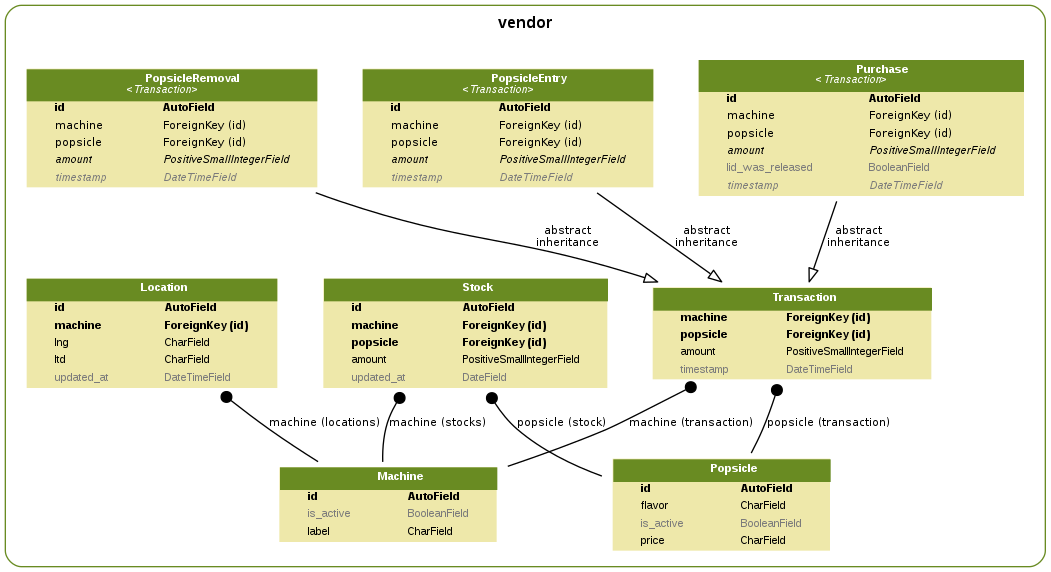
\includegraphics[width=\textwidth]{figuras/diagrama_classes}
% \caption{Diagrama de Classes}
% \label{fig:diagram_classes}
% \end{figure}

\begin{itemize}
\item \textit{Popsicle} representa um sabor de picolé e seu preço
\item \textit{Location} armazena as informações de latitude e longitude enviadas pelo GPS integrado à máquina
\item \textit{Machine} possui a localização física da máquina e o estoque de picolé
\item \textit{Stock} demonstra a quantidade de picolés de um determinado sabor, que existem em certa máquina.
\item \textit{User} simboliza um usuário do sistema, com informações como nome, login, senha e restrição de acesso (é administrador ou não). Como o cliente não precisará informar estes dados, somente administradores e vendedores são representados nesta classe.
\item \textit{Transaction} É a classe base de uma transação, armazena a data e a quantidade de picolés que foram removidos ou adicionados a um carrinho.
\item \textit{Purchase} corresponde a uma compra e herda de \textit{Transaction}.
\item \textit{PopsicleEntry} armazena uma entrada de picolés no estoque.
\item \textit{PopsicleRemoval} representa a remoção de picolés da máquina.
\end{itemize}

Além da arquitetura cliente-servidor, decidiu-se utilizar a arquitetura em camadas, bem típica de aplicações \textit{web}, no \textit{webservice}. O meio de interação entre o webapp e o servidor é uma API \textit{RESTful}.

O código da API desenvolvido encontra-se no \href{http://github.com/pi2-picole/api}{repositório} do grupo.


\subsection{WebApp}
\subsection{Implementação}

\subsubsection{Tecnologias}

As tecnologias utilizadas para a construção da interface que irá interagir diretamente com o cliente estão dispostas nesta seção. São elas:

\begin{itemize}
\item \textbf{Javascript:} As requisições para o \textit{webservice} foram feitas com o uso de uma biblioteca javascript denominada Jquery. A bilioteca foi utilizada para fazer tanto requisições do tipo GET, quanto do tipo POST. É por meio das requisições que se atualizam informações como estoque atual, localização das máquinas e faz todos os cadastros do sistema, em resumo, todas as interações que precisam atualizar o banco de dados e serviço de localização. Todos os eventos dinâmicos foram feitos na linguagem javascript.
\item \textbf{Google maps API:} A sigla API significa \textit{Application Programming Interface}, a google oferece diferentes APIs para serviços de localização, a utilizada no projeto é a API javascript do google maps, e os recursos são utilizados para obter a localização do usuário, a localização das máquinas através de latitude e longitude e calcular a rota até a máquina que o usuário escolher para efetivar a compra.
\item\textbf{ html 5 + css 3:} Foram utilizadas para a construção de toda a interface com o usuário. A parte da aplicação que usário realmente vê e interage é a que foi feita em html+css. Como a aplicação final é um \textit{webapp} a responsividade é indiscutivelmente importante, a aplicação tem que se comportar perfeitamente em dispositivos móveis, o html e o css são os responsáveis pela aplicação está completamente responsiva.
\item\textbf{Git:} O Git é um sistema de controle de versão distribuído gratuito, permite controlar as versões do código e que várias pessoas trabalhem na mesma funcionalidade.
\end{itemize}


A área de compra para o cliente, ficou de acordo com o definido na solução, e a interface do usuário ficou da seguinte forma:

\begin{itemize}
\item

\subsubsection{Página Inicial}

% \begin{figure}[H]
% 	\centering
%     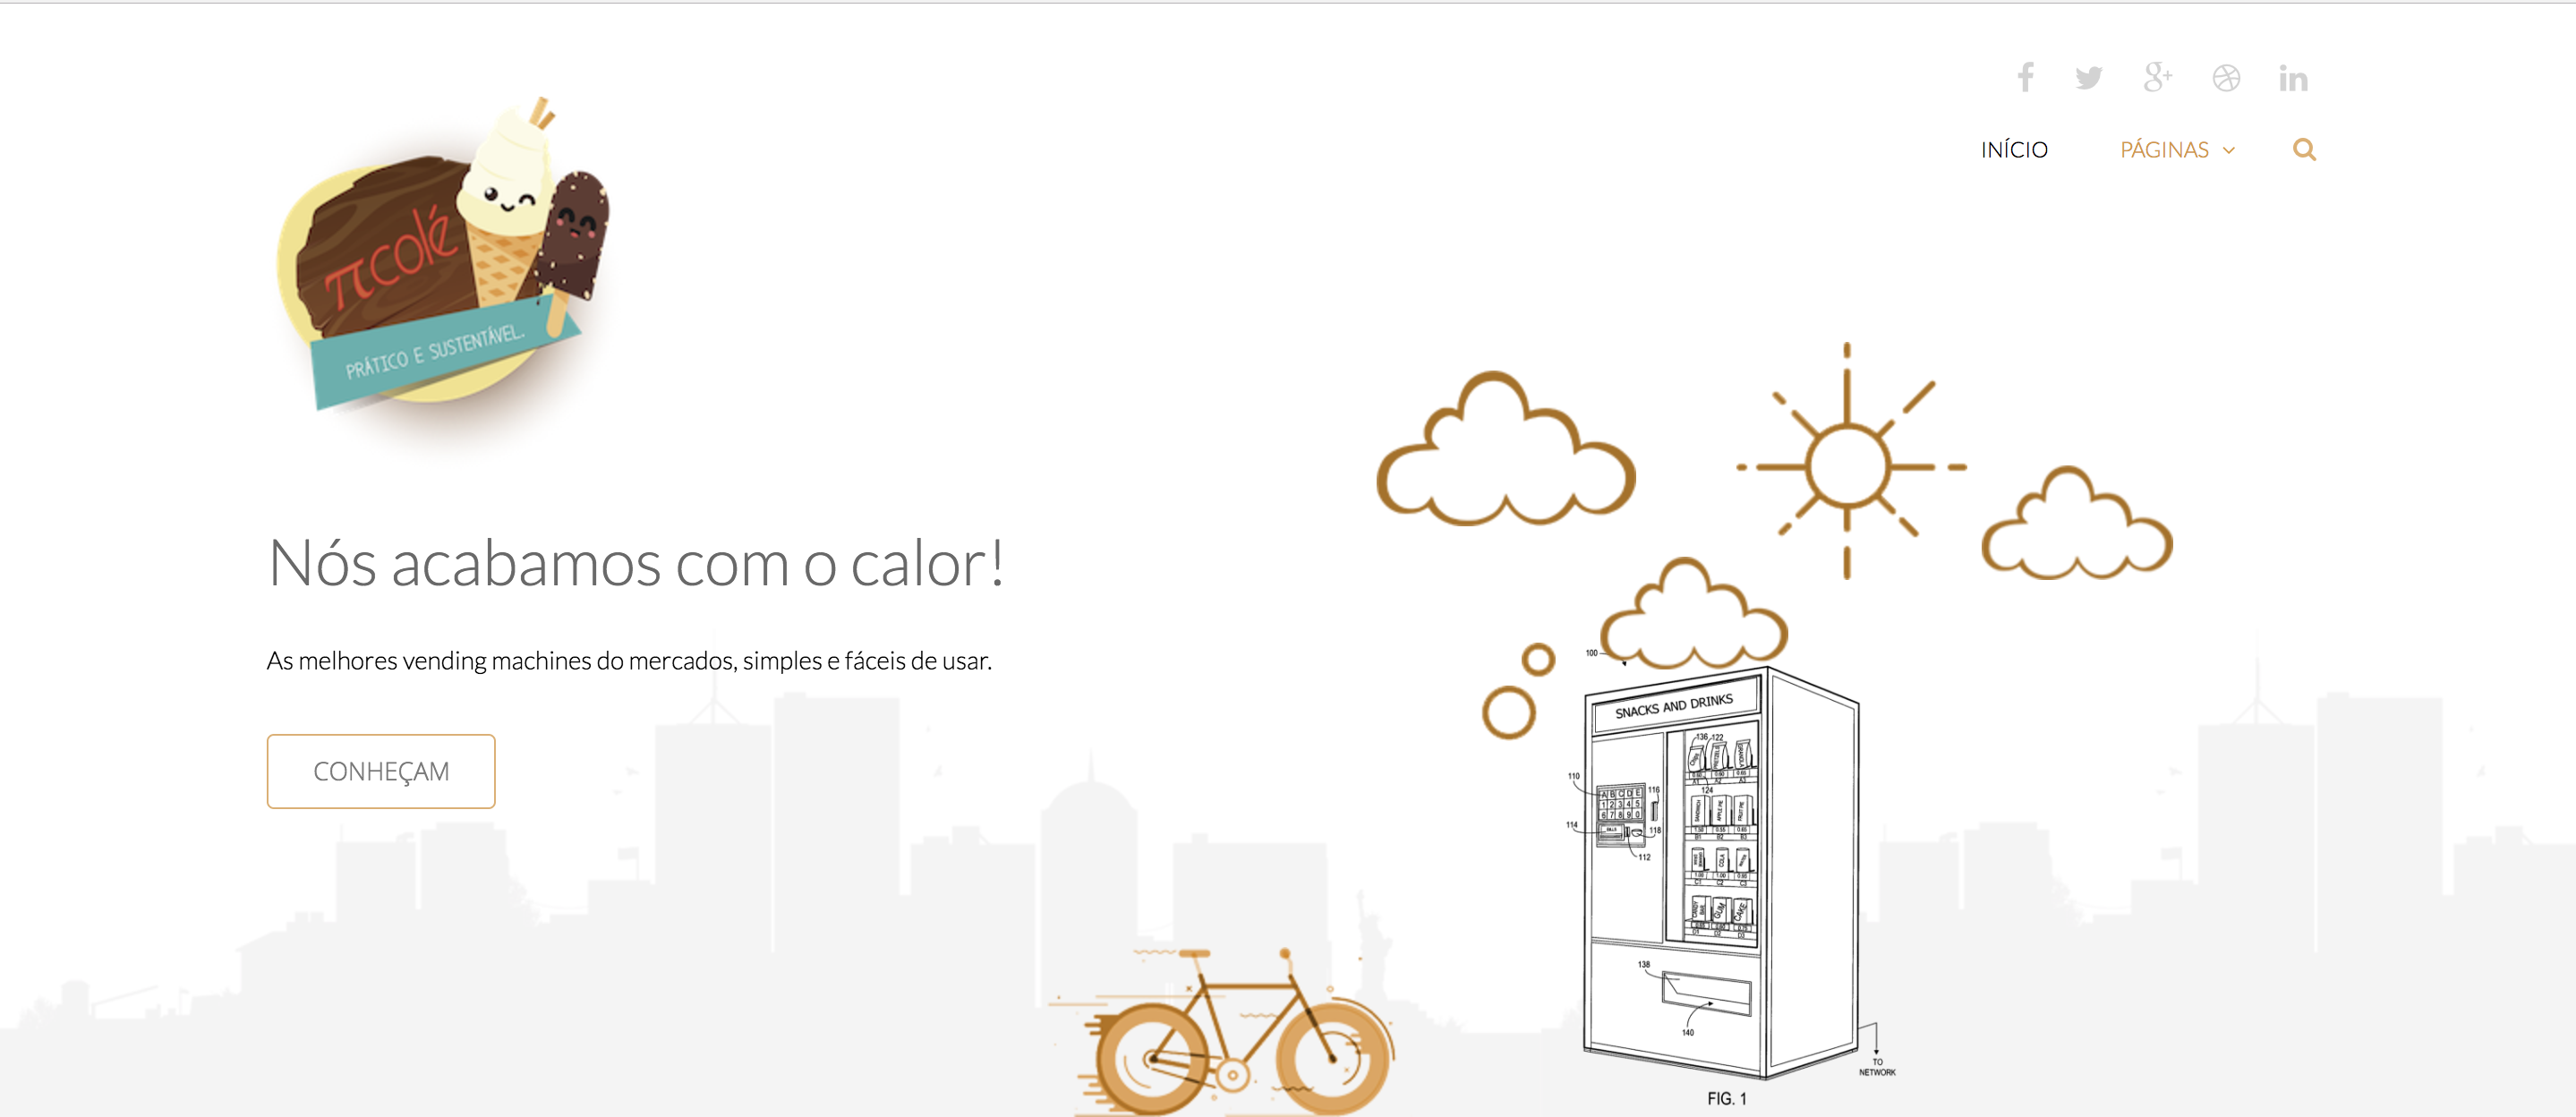
\includegraphics[width=\textwidth]{figuras/inicio}
%     \caption{Página Inicial}
%     \label{fig:Página Inicial}
% \end{figure}

Essa é a tela inicial do webapp, proporcionando uma primeira idéia do que se trata o site.

\item{Mapa de máquinas}

% \begin{figure}[H]
% 	\centering
%     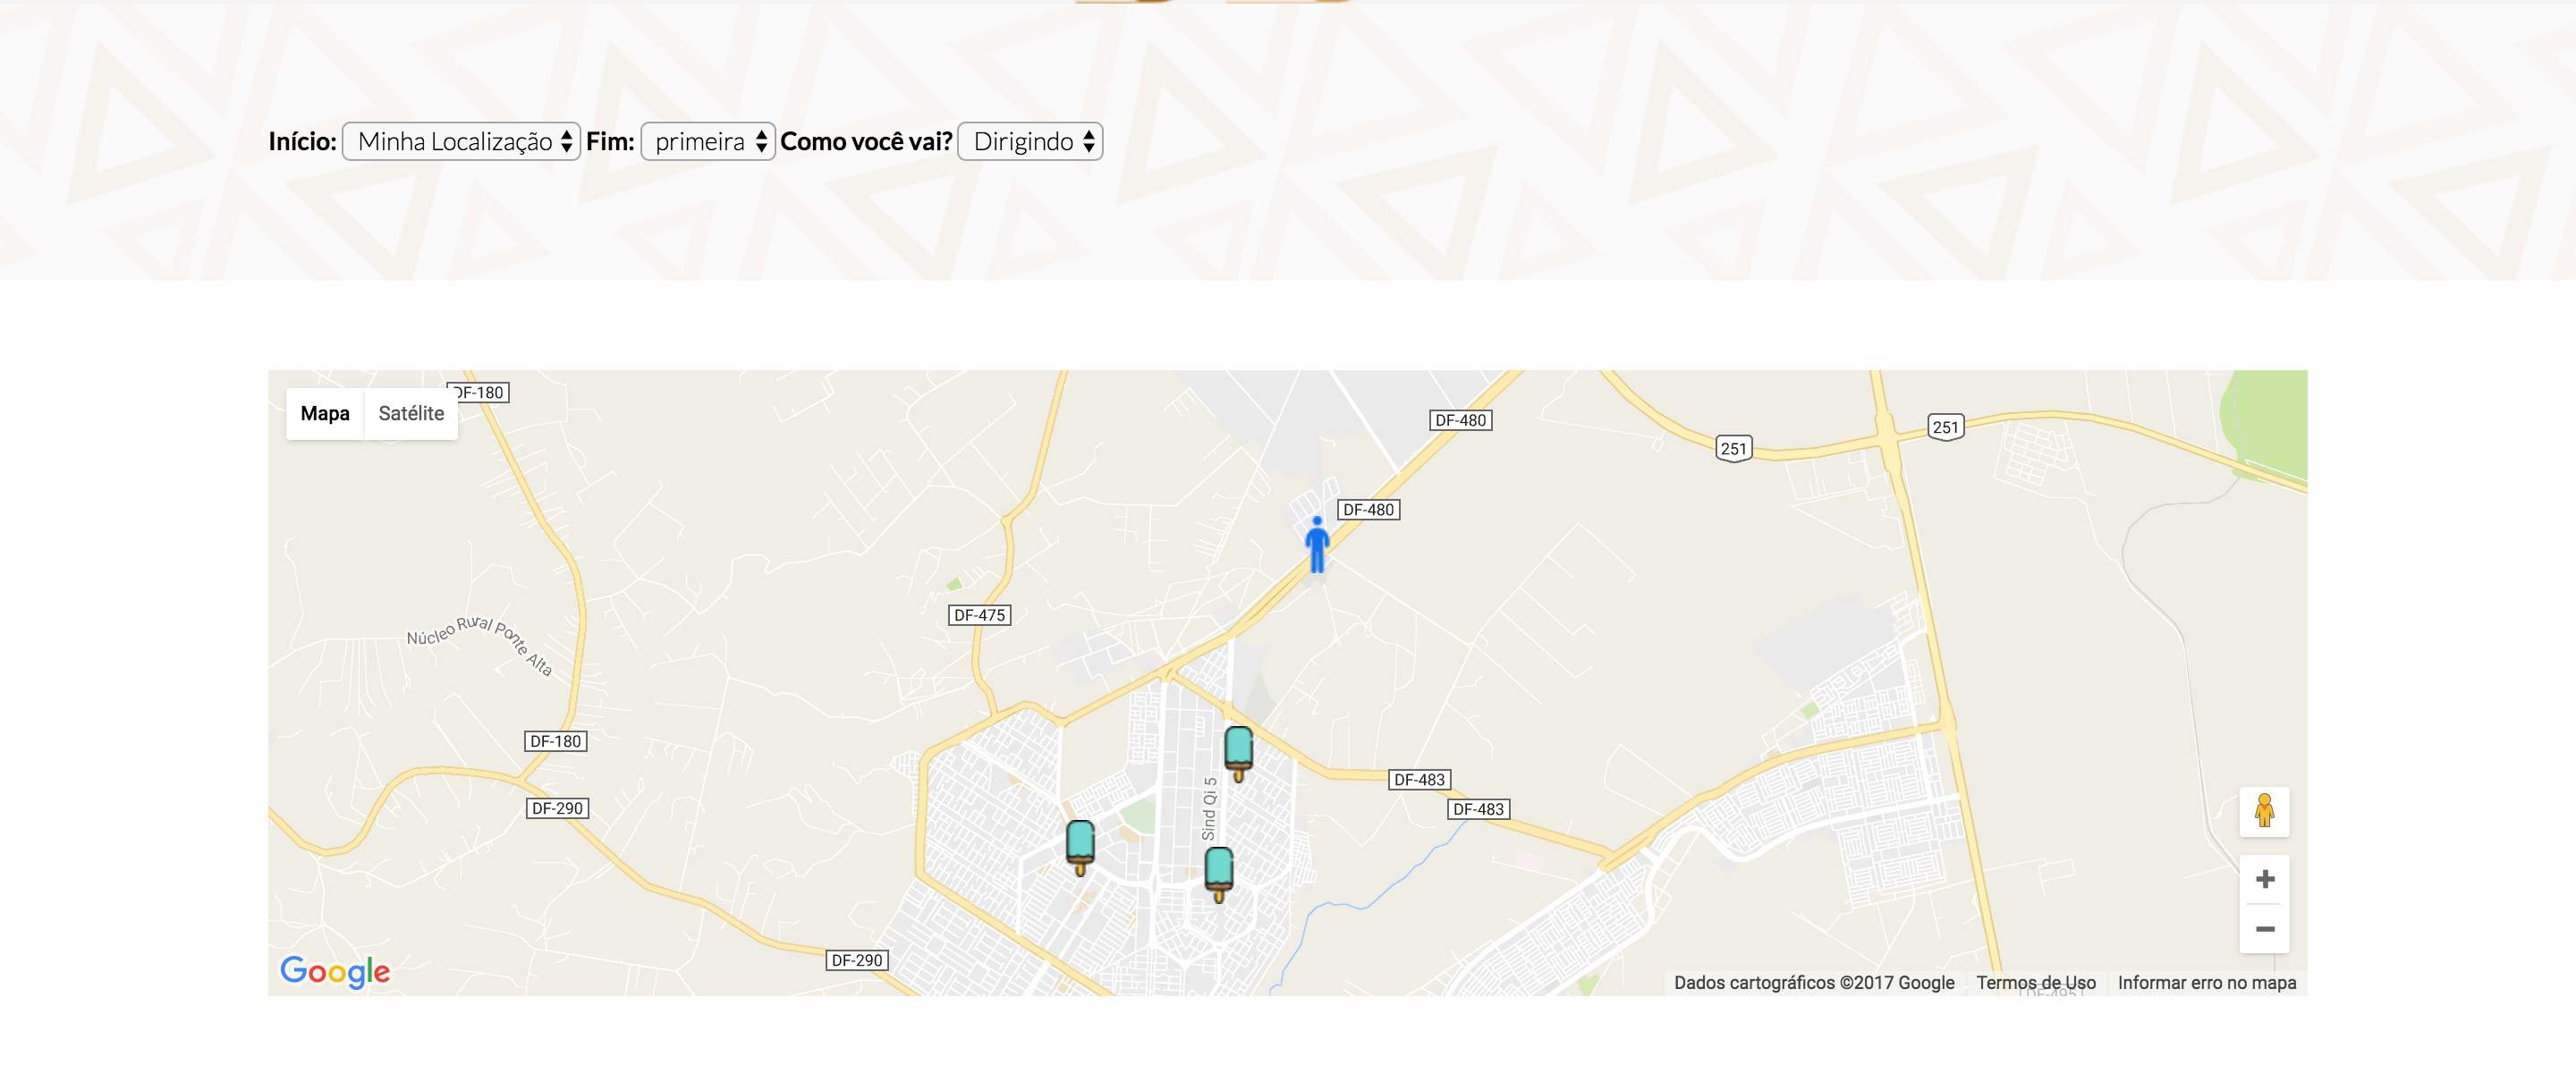
\includegraphics[width=\textwidth]{figuras/map}
%     \caption{Mapa de máquinas}
%     \label{fig:Mapa de máquinas}
% \end{figure}

Diretamente embaixo do item acima, se encontra o mapa, onde estão sendo mostradas as máquinas disponíveis para serem comprados os picolés.

\item{Mapa de máquinas (Com Rota)}

% \begin{figure}[H]
% 	\centering
%     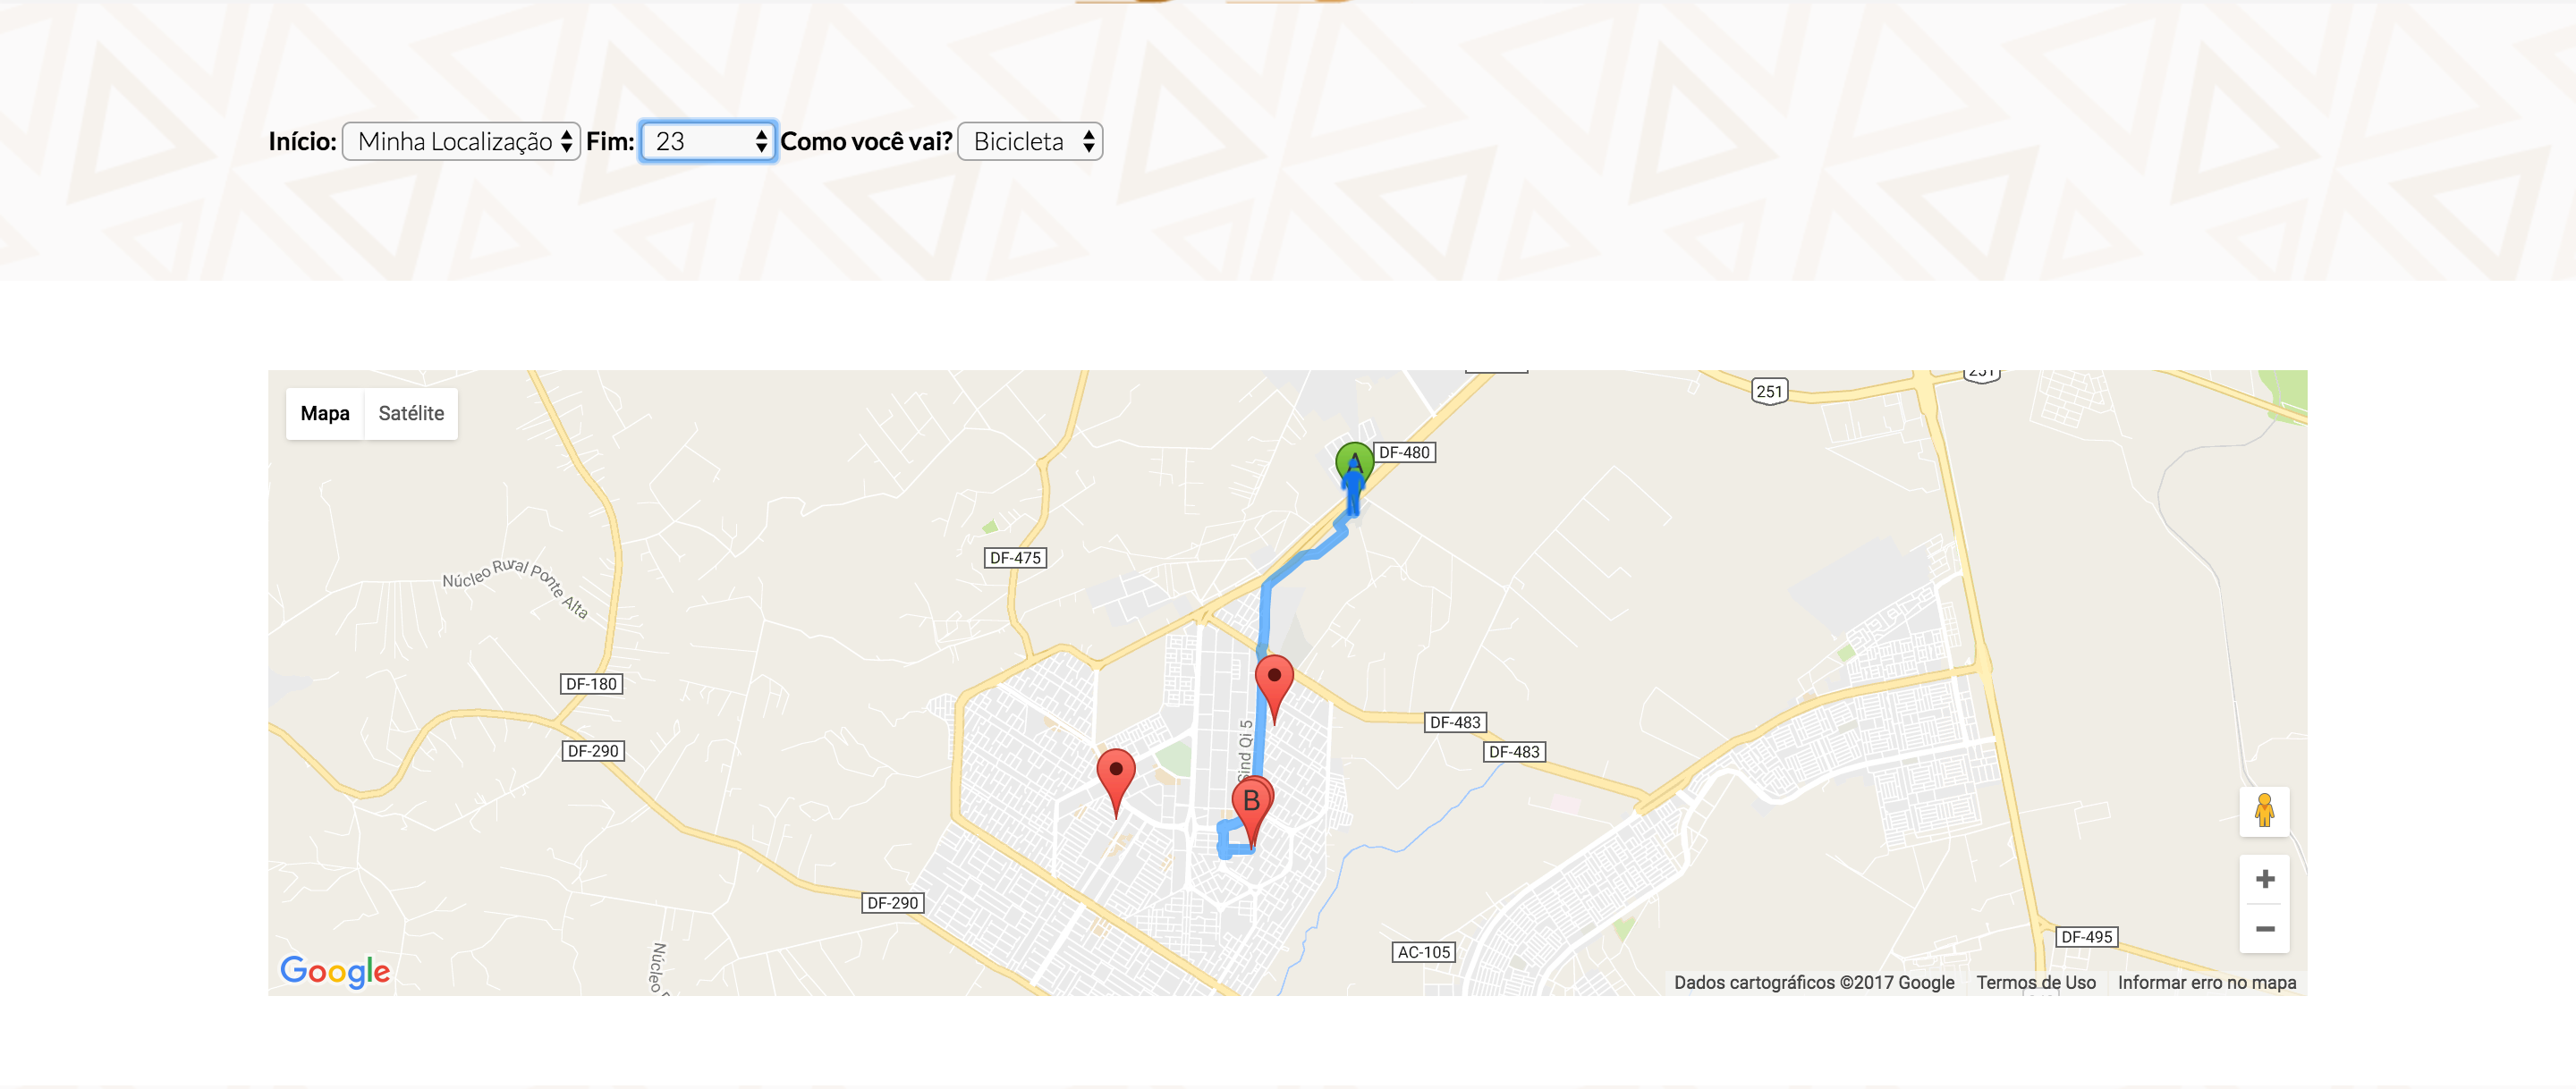
\includegraphics[width=\textwidth]{figuras/rotas}
%     \caption{Mapa de máquinas, com rotas}
%     \label{fig:Mapa de máquinas, com rotas}
% \end{figure}

Nesta figura se encontra a seleção de uma máquina e a definição da melhor rota para a máquina escolhida pelo cliente.


\item{Seleção de sabores e quantidade}

% \begin{figure}[H]
% 	\centering
%     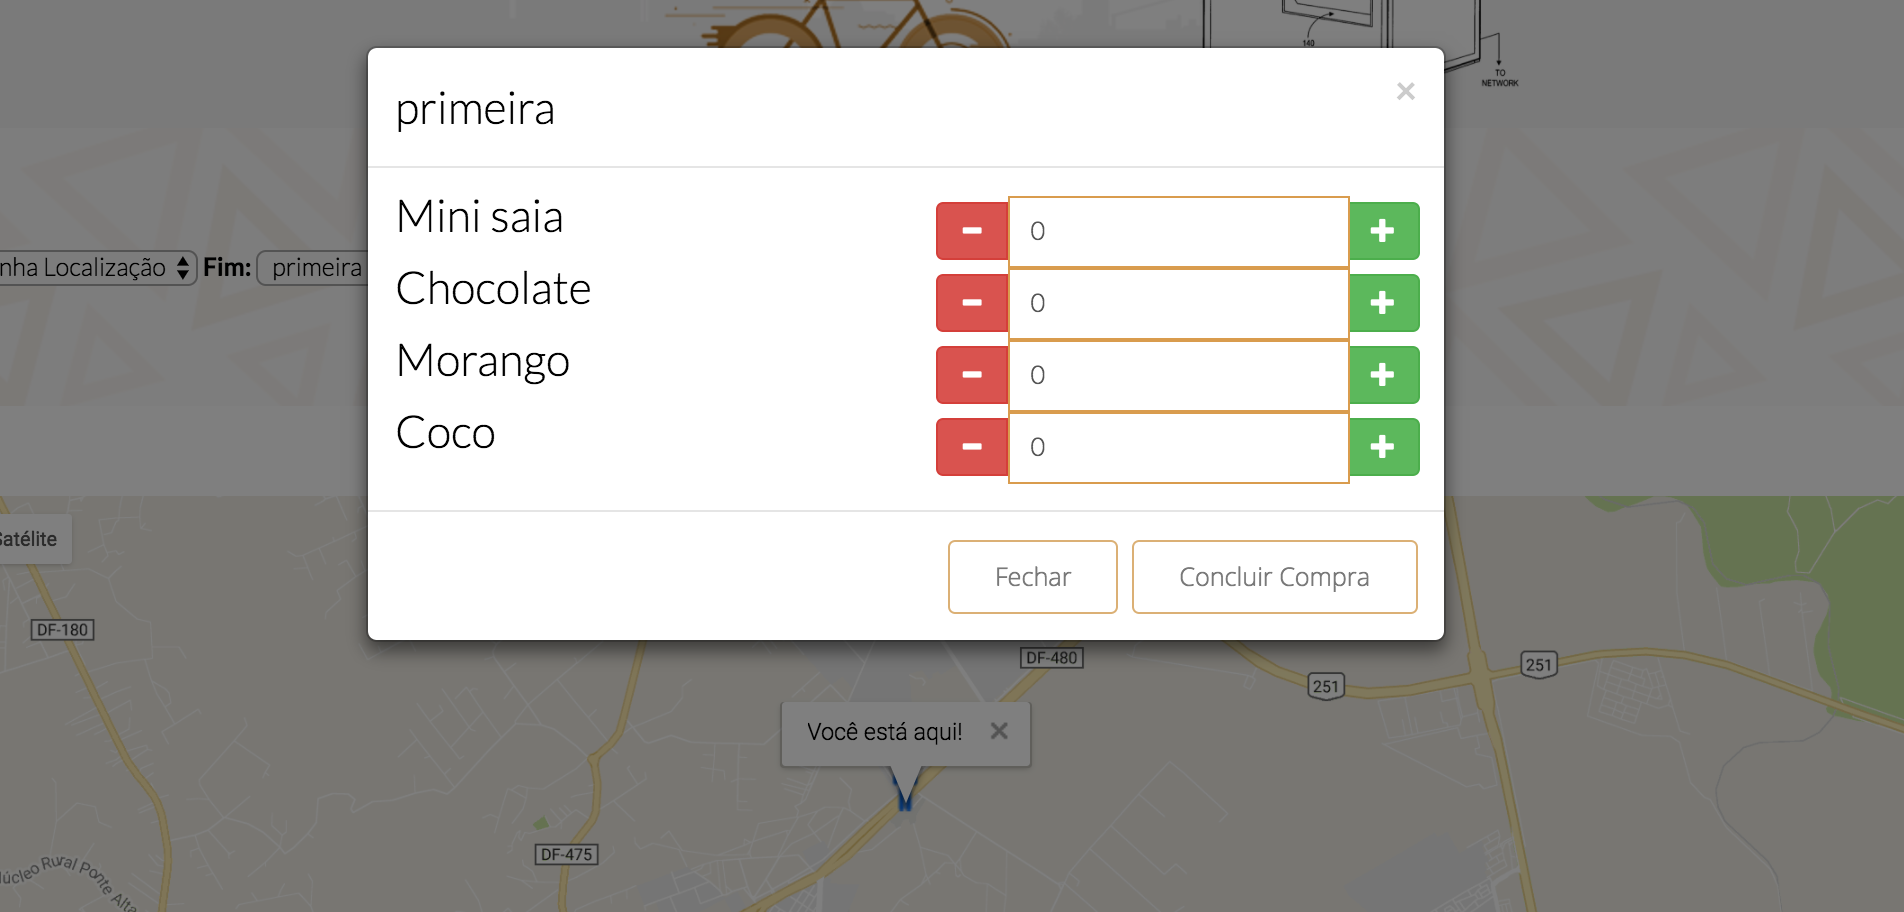
\includegraphics[width=\textwidth]{figuras/quantidade}
%     \caption{Seleção de sabores}
%     \label{fig:Seleção de sabores}
% \end{figure}

Selecionada a máquina na qual se deseja fazer a compra, e clicando no marcador correspondente, o popup acima aparece, possibilitando ao cliente selecionar os sabores e as quantidades de cada um.


\item{Tela de pagamento}

% \begin{figure}[H]
% 	\centering
%     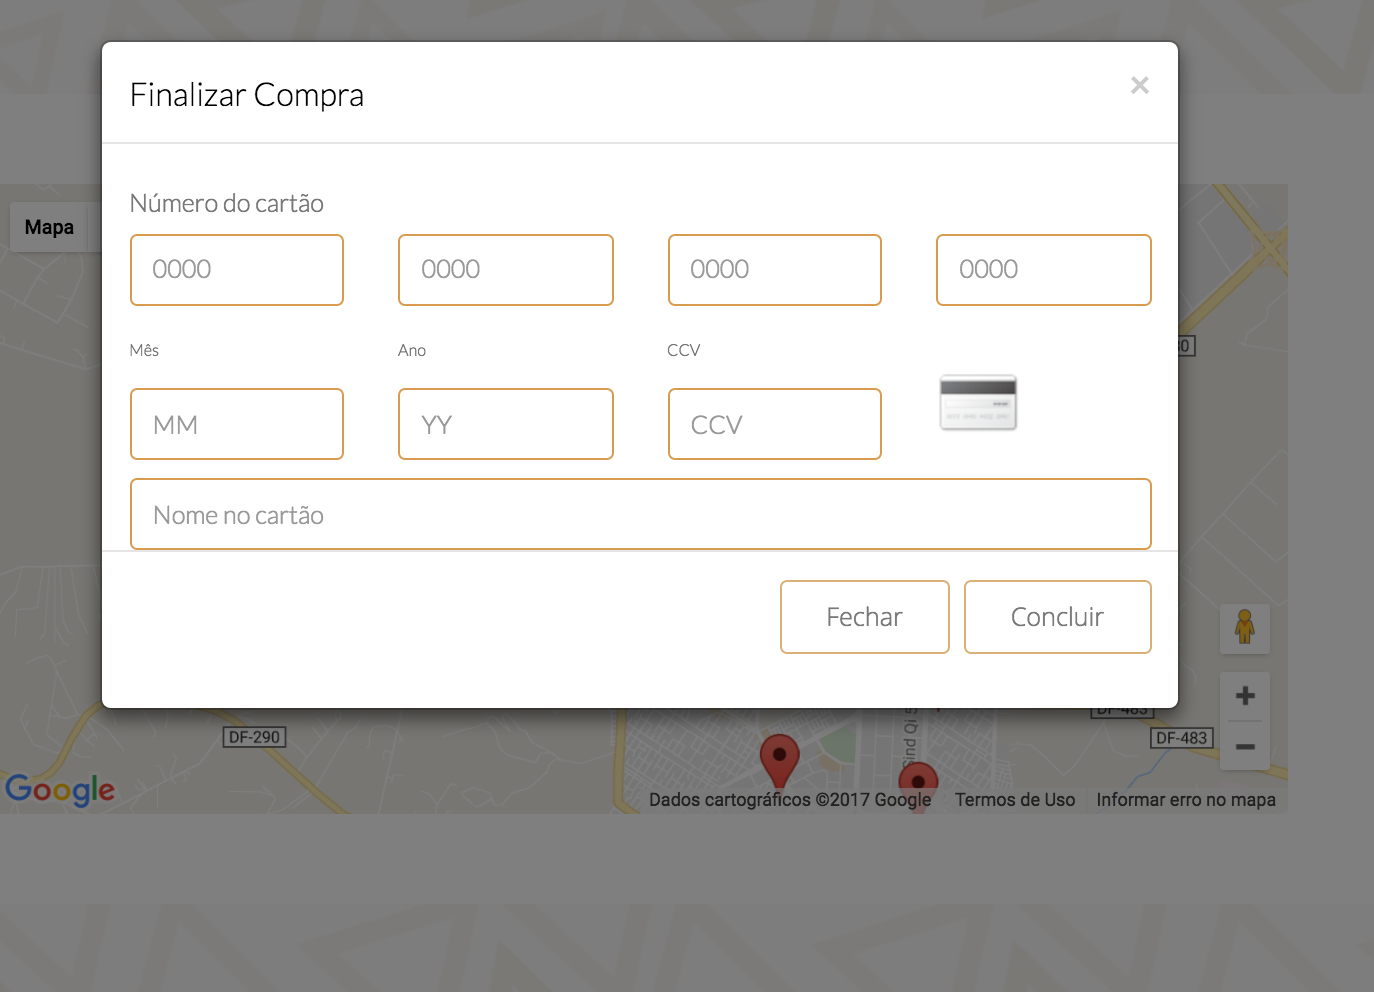
\includegraphics[width=\textwidth]{figuras/cartao}
%     \caption{Tela De Pagamento}
%     \label{fig:Tela de pagamento}
% \end{figure}

Após selecionados, e clicado no botão, a tela de pagamento é mostrada, o cliente deve entrar com os seus dados e finalizar a compra.

Como definido anteriormente, foram definidos cadastros e estoque para as áreas de vendedor e administrador. As interfaces de cadastro e estoque são as seguintes:

\item{Cadastro de Máquinas}

% \begin{figure}[H]
% 	\centering
%     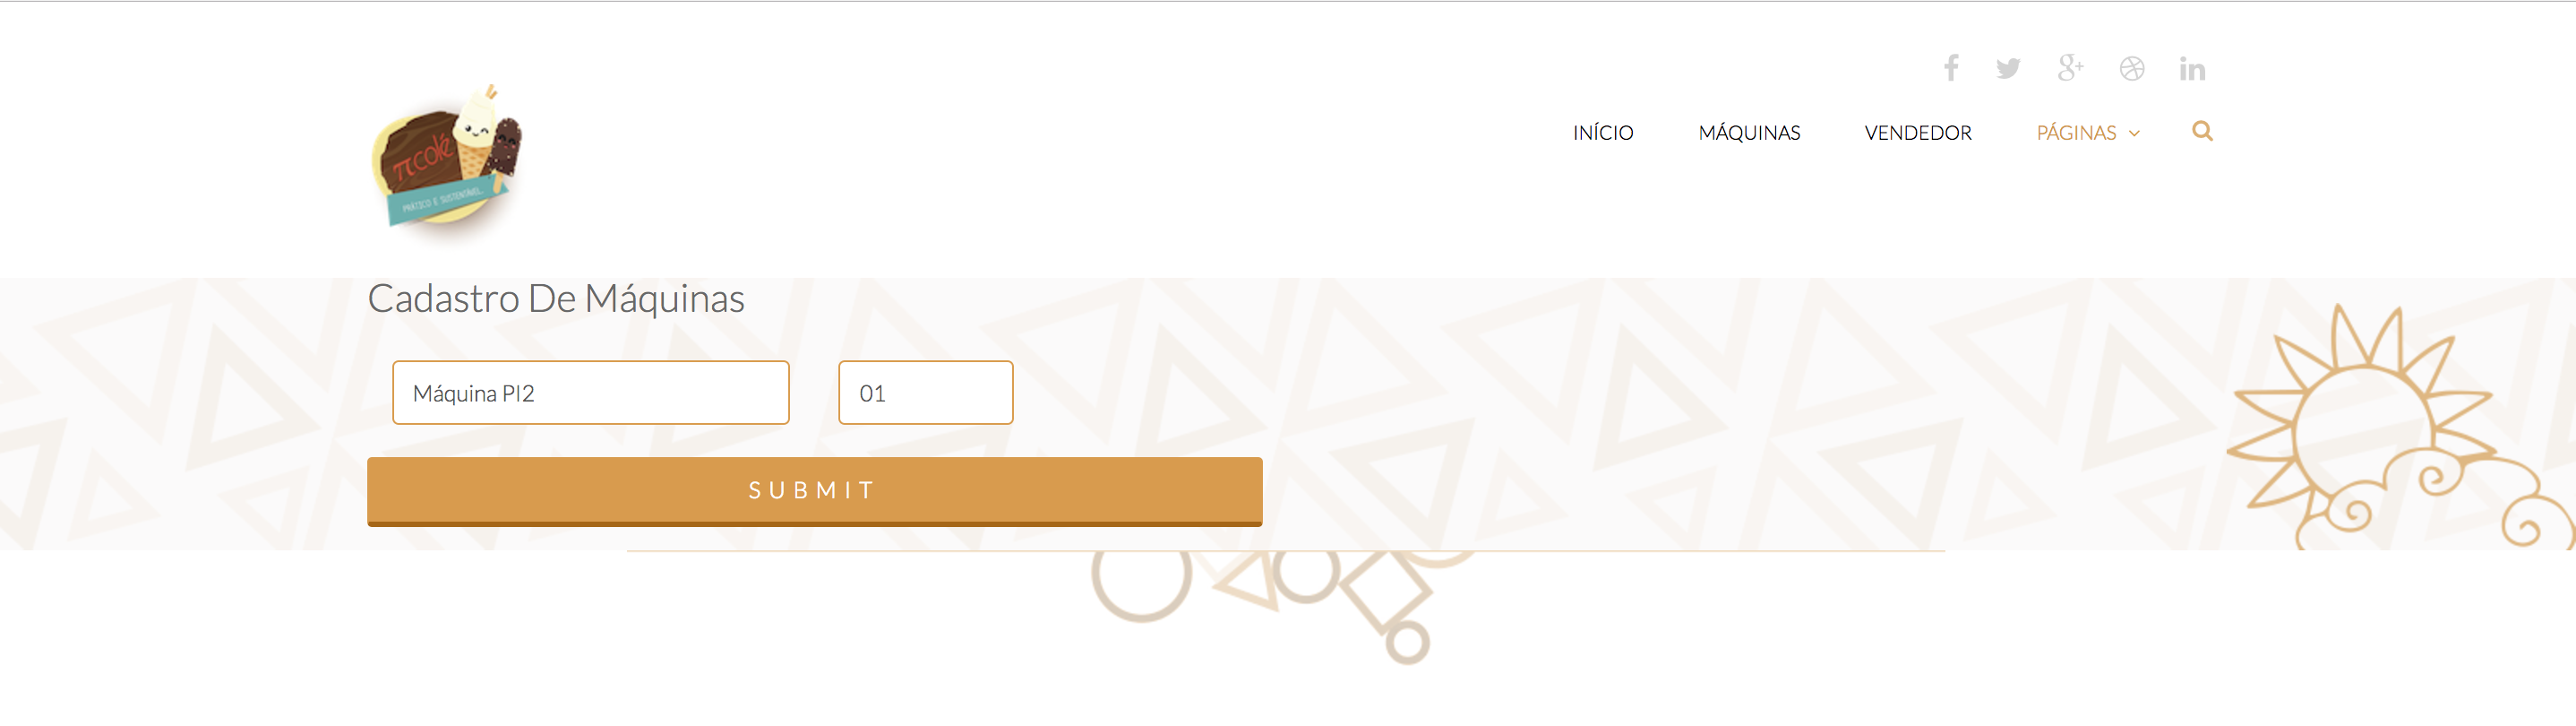
\includegraphics[width=\textwidth]{figuras/cadastroMaquinas}
%     \caption{Cadastro de Máquinas}
%     \label{fig:CadastroMaquinas}
% \end{figure}

Na área de administrador, é possível cadastrar máquinas por meio dessa interface.

\item{Cadastro de Vendedor}

% \begin{figure}[H]
% 	\centering
%     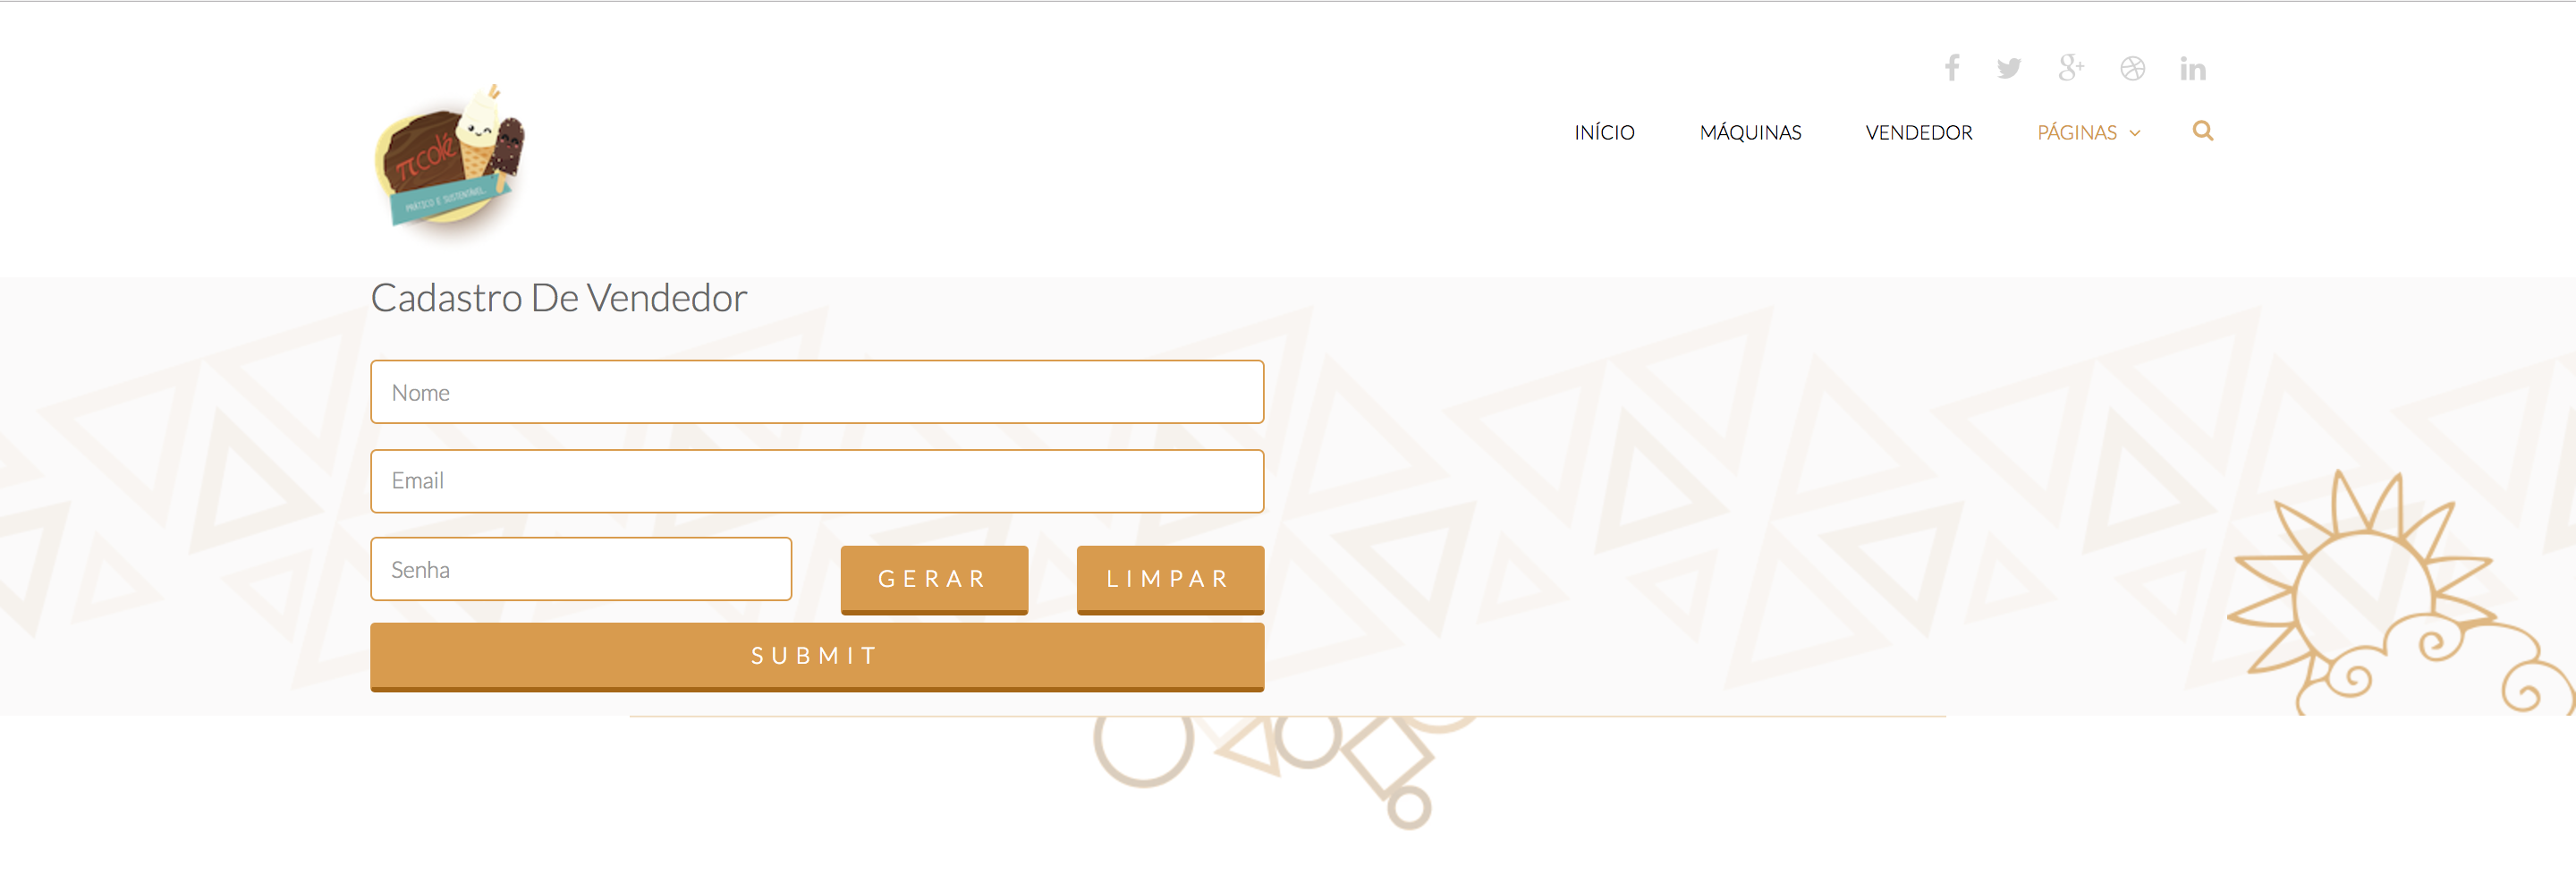
\includegraphics[width=\textwidth]{figuras/cadastroVendedor}
%     \caption{Cadastro de Vendedor}
%     \label{fig:CadastroMaquinas}
% \end{figure}

Nesta tela, é possível cadastrar vendedores.

\item{Cadastro de Sabores}

% \begin{figure}[H]
% 	\centering
%     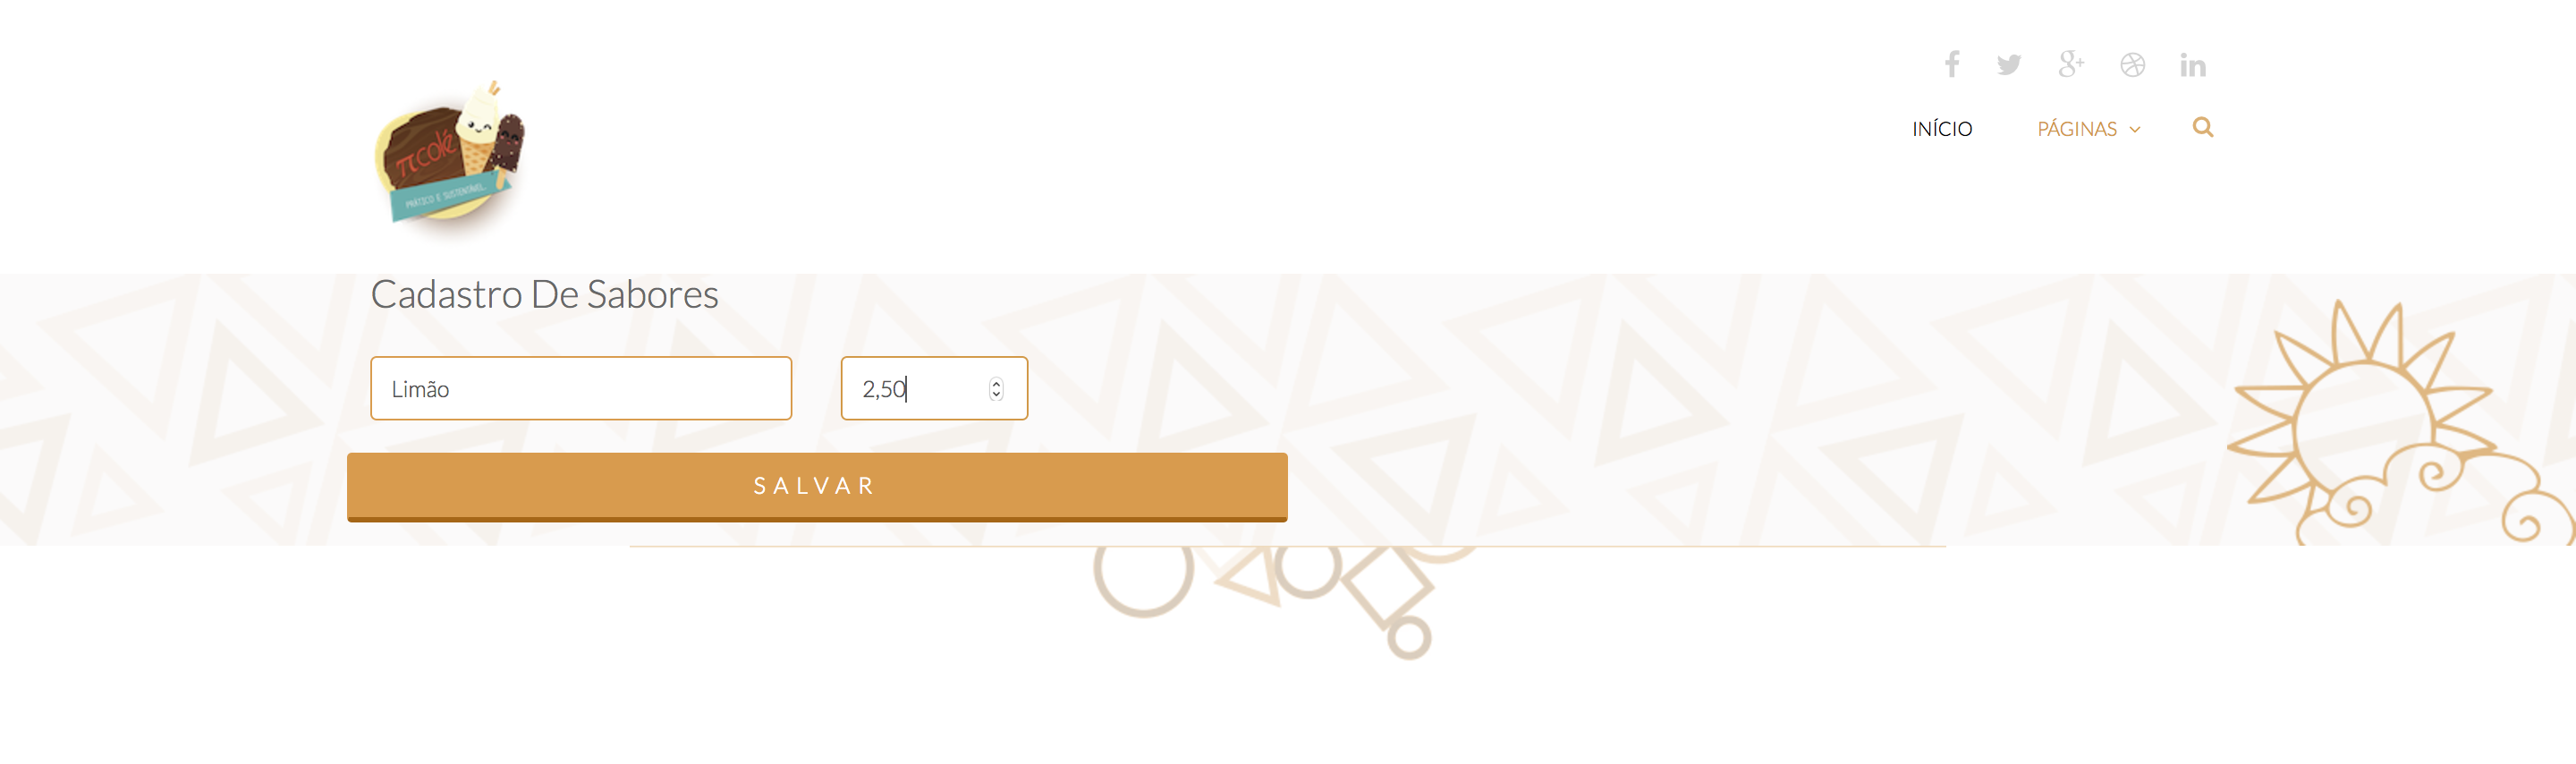
\includegraphics[width=\textwidth]{figuras/cadastroSabores}
%     \caption{Cadastro de Sabores}
%     \label{fig:CadastroMaquinas}
% \end{figure}

Nesta tela, o administrador pode cadastrar sabores de picolé.

\item{Estoque}

% \begin{figure}[H]
% 	\centering
%     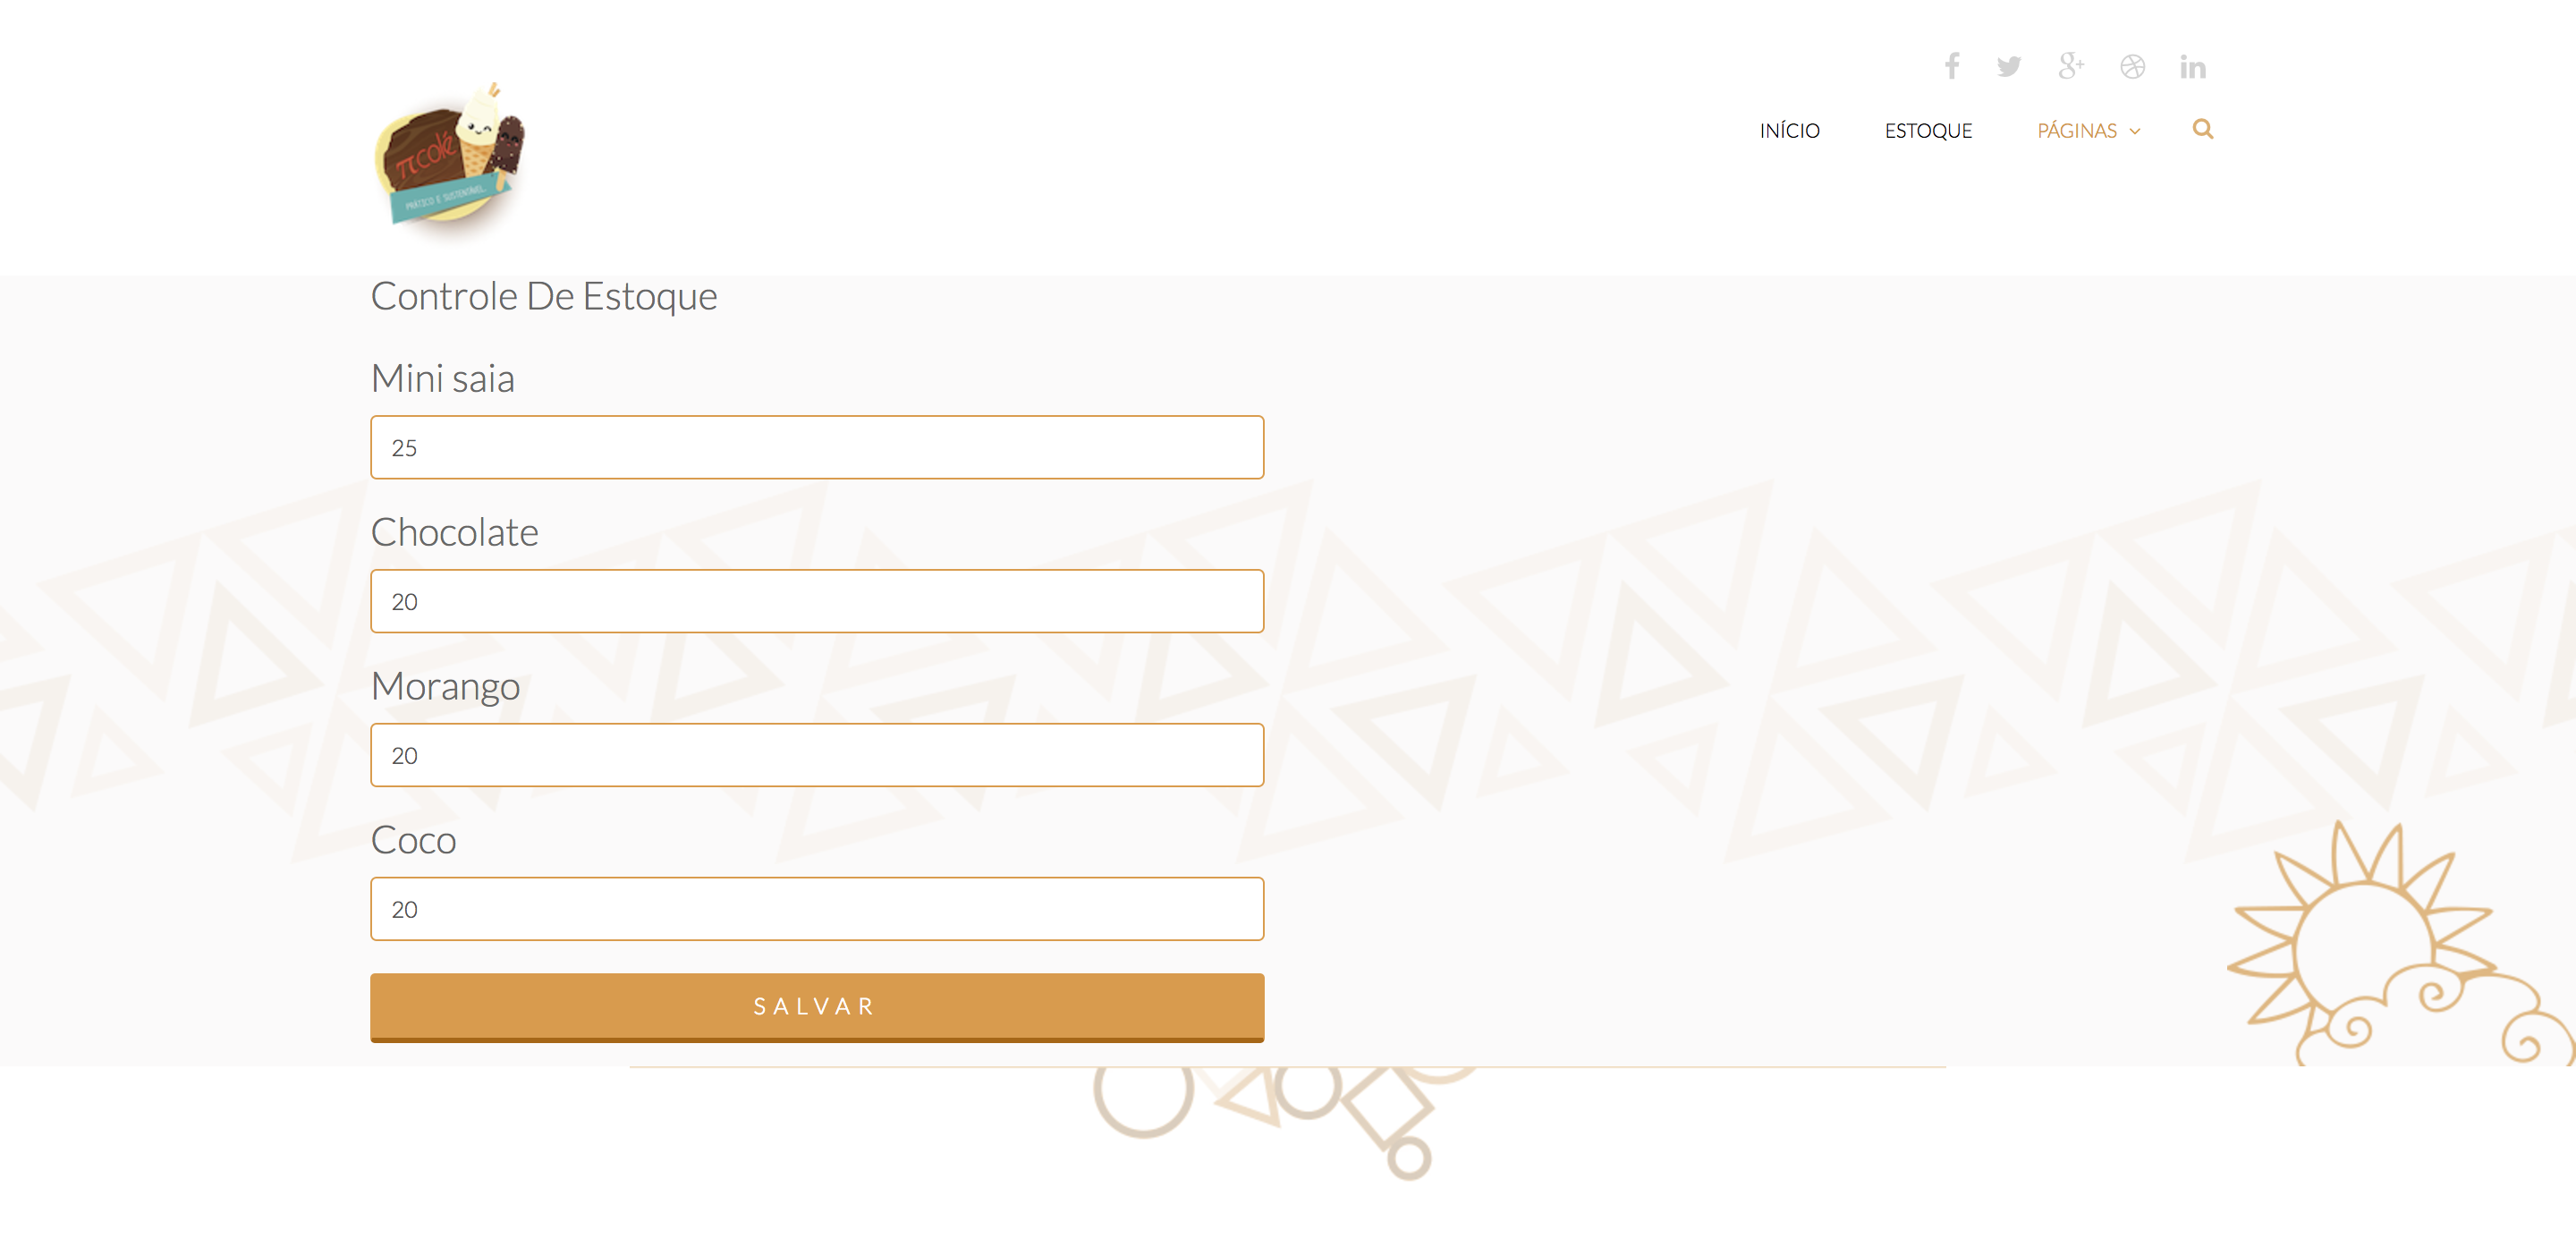
\includegraphics[width=\textwidth]{figuras/storage}
%     \caption{Gerenciamento de estoque}
%     \label{fig:CadastroMaquinas}
% \end{figure}

Nesta interface, o vendedor pode gerenciar seu estoque.

\end{itemize}

\section{Solução de Eletrônica}

A parte eletrônica da máquina de vendas de picolé é dividida nos seguintes sistemas:

\subsection{Sistema GPS e Segurança}

A máquina de vendas terá um sistema de segurança utilizando-se um sistema de posicionamento global (GPS). O dispositivo GPS utilizado é o módulo da família de GPS U-blox stand-alone com chip GY-NEO6MV2 integrado. A plataforma escolhida para adquirir os dados de posicionamento foi o Arduino devido à facilidade de implementação com bibliotecas já prontas. 

\subsubsection{Implementação}

Para a comunicação do módulo GPS, é necessário o uso de duas bibliotecas. A primeira delas é a SoftwareSerial.h, a qual permite a comunicação serial em outros pinos digitais do Arduino por meio de software, já que os dados transmitidos pelo módulo é via serial full-duplex de dois fios. Já a biblioteca TinyGps.h fornece as funcionalidades como posição e curso com códigos mais simples, além de manter o recurso em baixo consumo e tratar sinais de pontos flutuantes.

\subsubsection{Teste}
Para a realização do teste, utilizou-se a seguinte montagem (criado com o software Fritzing):

\begin{figure}[H]
	\centering
    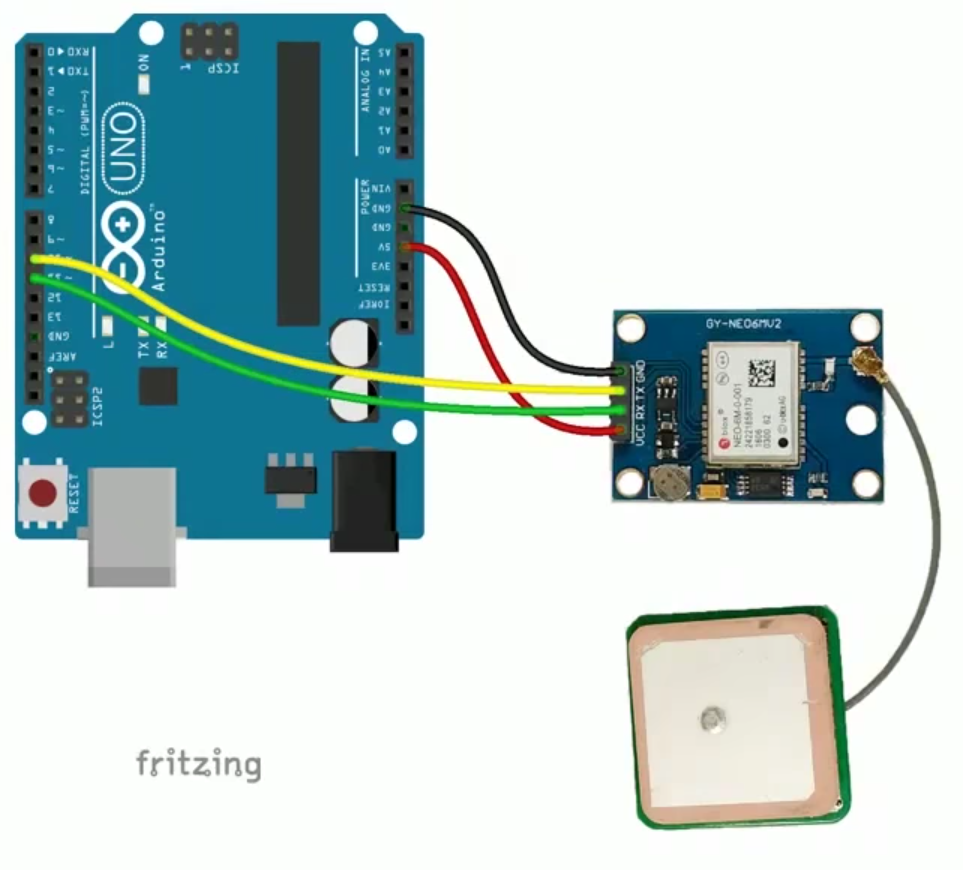
\includegraphics[width=0.7\textwidth]{figuras/fritzing_arduino}
    \caption{Esquema de montagem do GPS para teste no Arduino}
    \label{fig:fritzing_arduino}
\end{figure}

O GPS funcionou como esperado e retornou os valores de latitude e longitude com perfeita precisão. Porém, seu alcance é limitado, pois o sinal do GPS na UNB Faculdade Gama é alcançada em alguns pontos específicos.  

\subsection{Sistema de Som e Alarme}

Para o sistema de segurança integrado ao projeto, é necessário emitir um alarme caso a máquina de vendas seja violado ou removido do local designado pelo vendedor. Além disso, há um assistente com voz automática para receber um cliente próximo à máquina de vendas e, quando não houver nenhuma pessoa por perto, o sistema emite uma propaganda do produto. O sistema de som é responsável por atender os clientes quando estes se aproximam, fazer propaganda e alarmar em caso de violação.

Para isso, foi montado um circuito amplificador com o CI TDA8571, o qual é um amplificador dedicado capaz de oferecer 40 W para até 4 alto falantes de 4 Ohms cada. Como sua alimentação é de 12V DC, é ideal para o projeto.

\subsubsection{Implementação}

O esquemático do circuito montado foi retirado do Datasheet \cite{mq2} e está esquematizado a seguir:

\begin{figure}[H]
	\centering
    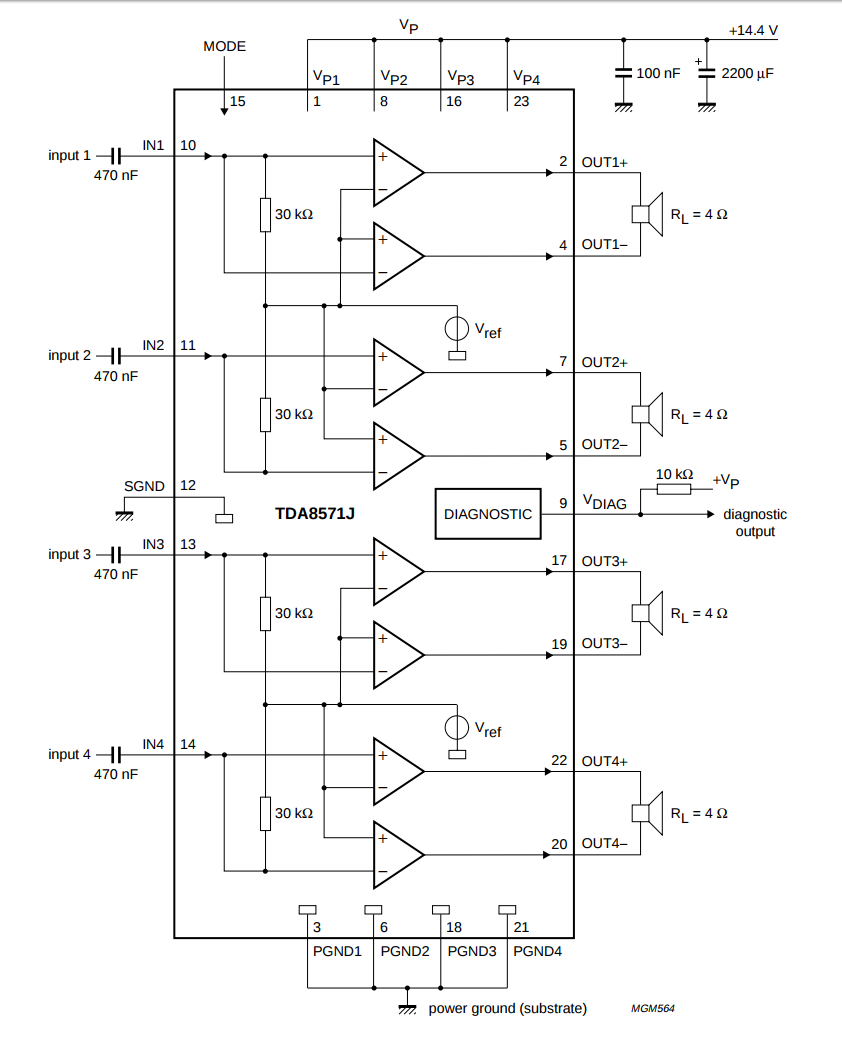
\includegraphics[width=\textwidth]{figuras/circuito_TDA}
    \caption{Esquemático utilizado para o circuito do amplificador de som}
    \label{fig:circuito_TDA}
\end{figure}

O circuito integrado é constituído de 8 amplificadores ligados em ponte, como mostrado acima. Além disso, foi acrescentado um fusível de 8A e um diodo na entrada para proteção contra curto circuito e inversão de polaridade. Os pinos foram ligados conforme esquematizado a seguir:

\begin{itemize}
	\item \textbf{Pino 15:} Pino de modo (mute e enable) que ativa ou desativa a saída. Foi ligado ao Raspberry para o controle de som.
    \item \textbf{Pinos 3, 6, 18, 21:} Alimentação negativa (terra 0 V) de cada um dos amplificadores.
    \item \textbf{Pinos 1, 8, 16, 23:} Alimentação positiva de cada um dos amplificadores. Foi utilizado 12 V, que é a tensão da fonte disponível do projeto.
    \item \textbf{Pinos 10, 11, 13, 14:} São as entradas de áudio. Como o áudio é o mesmo para todas as saídas, estes pinos estão em curto-circuito. O áudio vem do Raspberry Pi.
    \item \textbf{Pino 2, 4, 5, 7, 17, 19, 20, 22:} São as saídas de áudio. Foram ligados 4 alto falantes de 4 $\Omega$.
    \item \textbf{Pino 12:} Pino GND, foi ligado ao 0 V.
\end{itemize}

Os capacitores de 100 nF e 2200 $\mu$F servem para filtrar \textit{ripples} (oscilações) repentinas na fonte. Os capacitores de 470 nF retira o nível DC nas entradas de áudio. 

\subsubsection{Teste}

O circuito foi testado na protboard e funcionou com sucesso. As quatro saídas estão gerando sinais estáveis, o áudio é de boa qualidade e a intensidade do som é suficiente para o projeto. A seguir, o circuito montado na protoboard:

\begin{figure}[H]
	\centering
    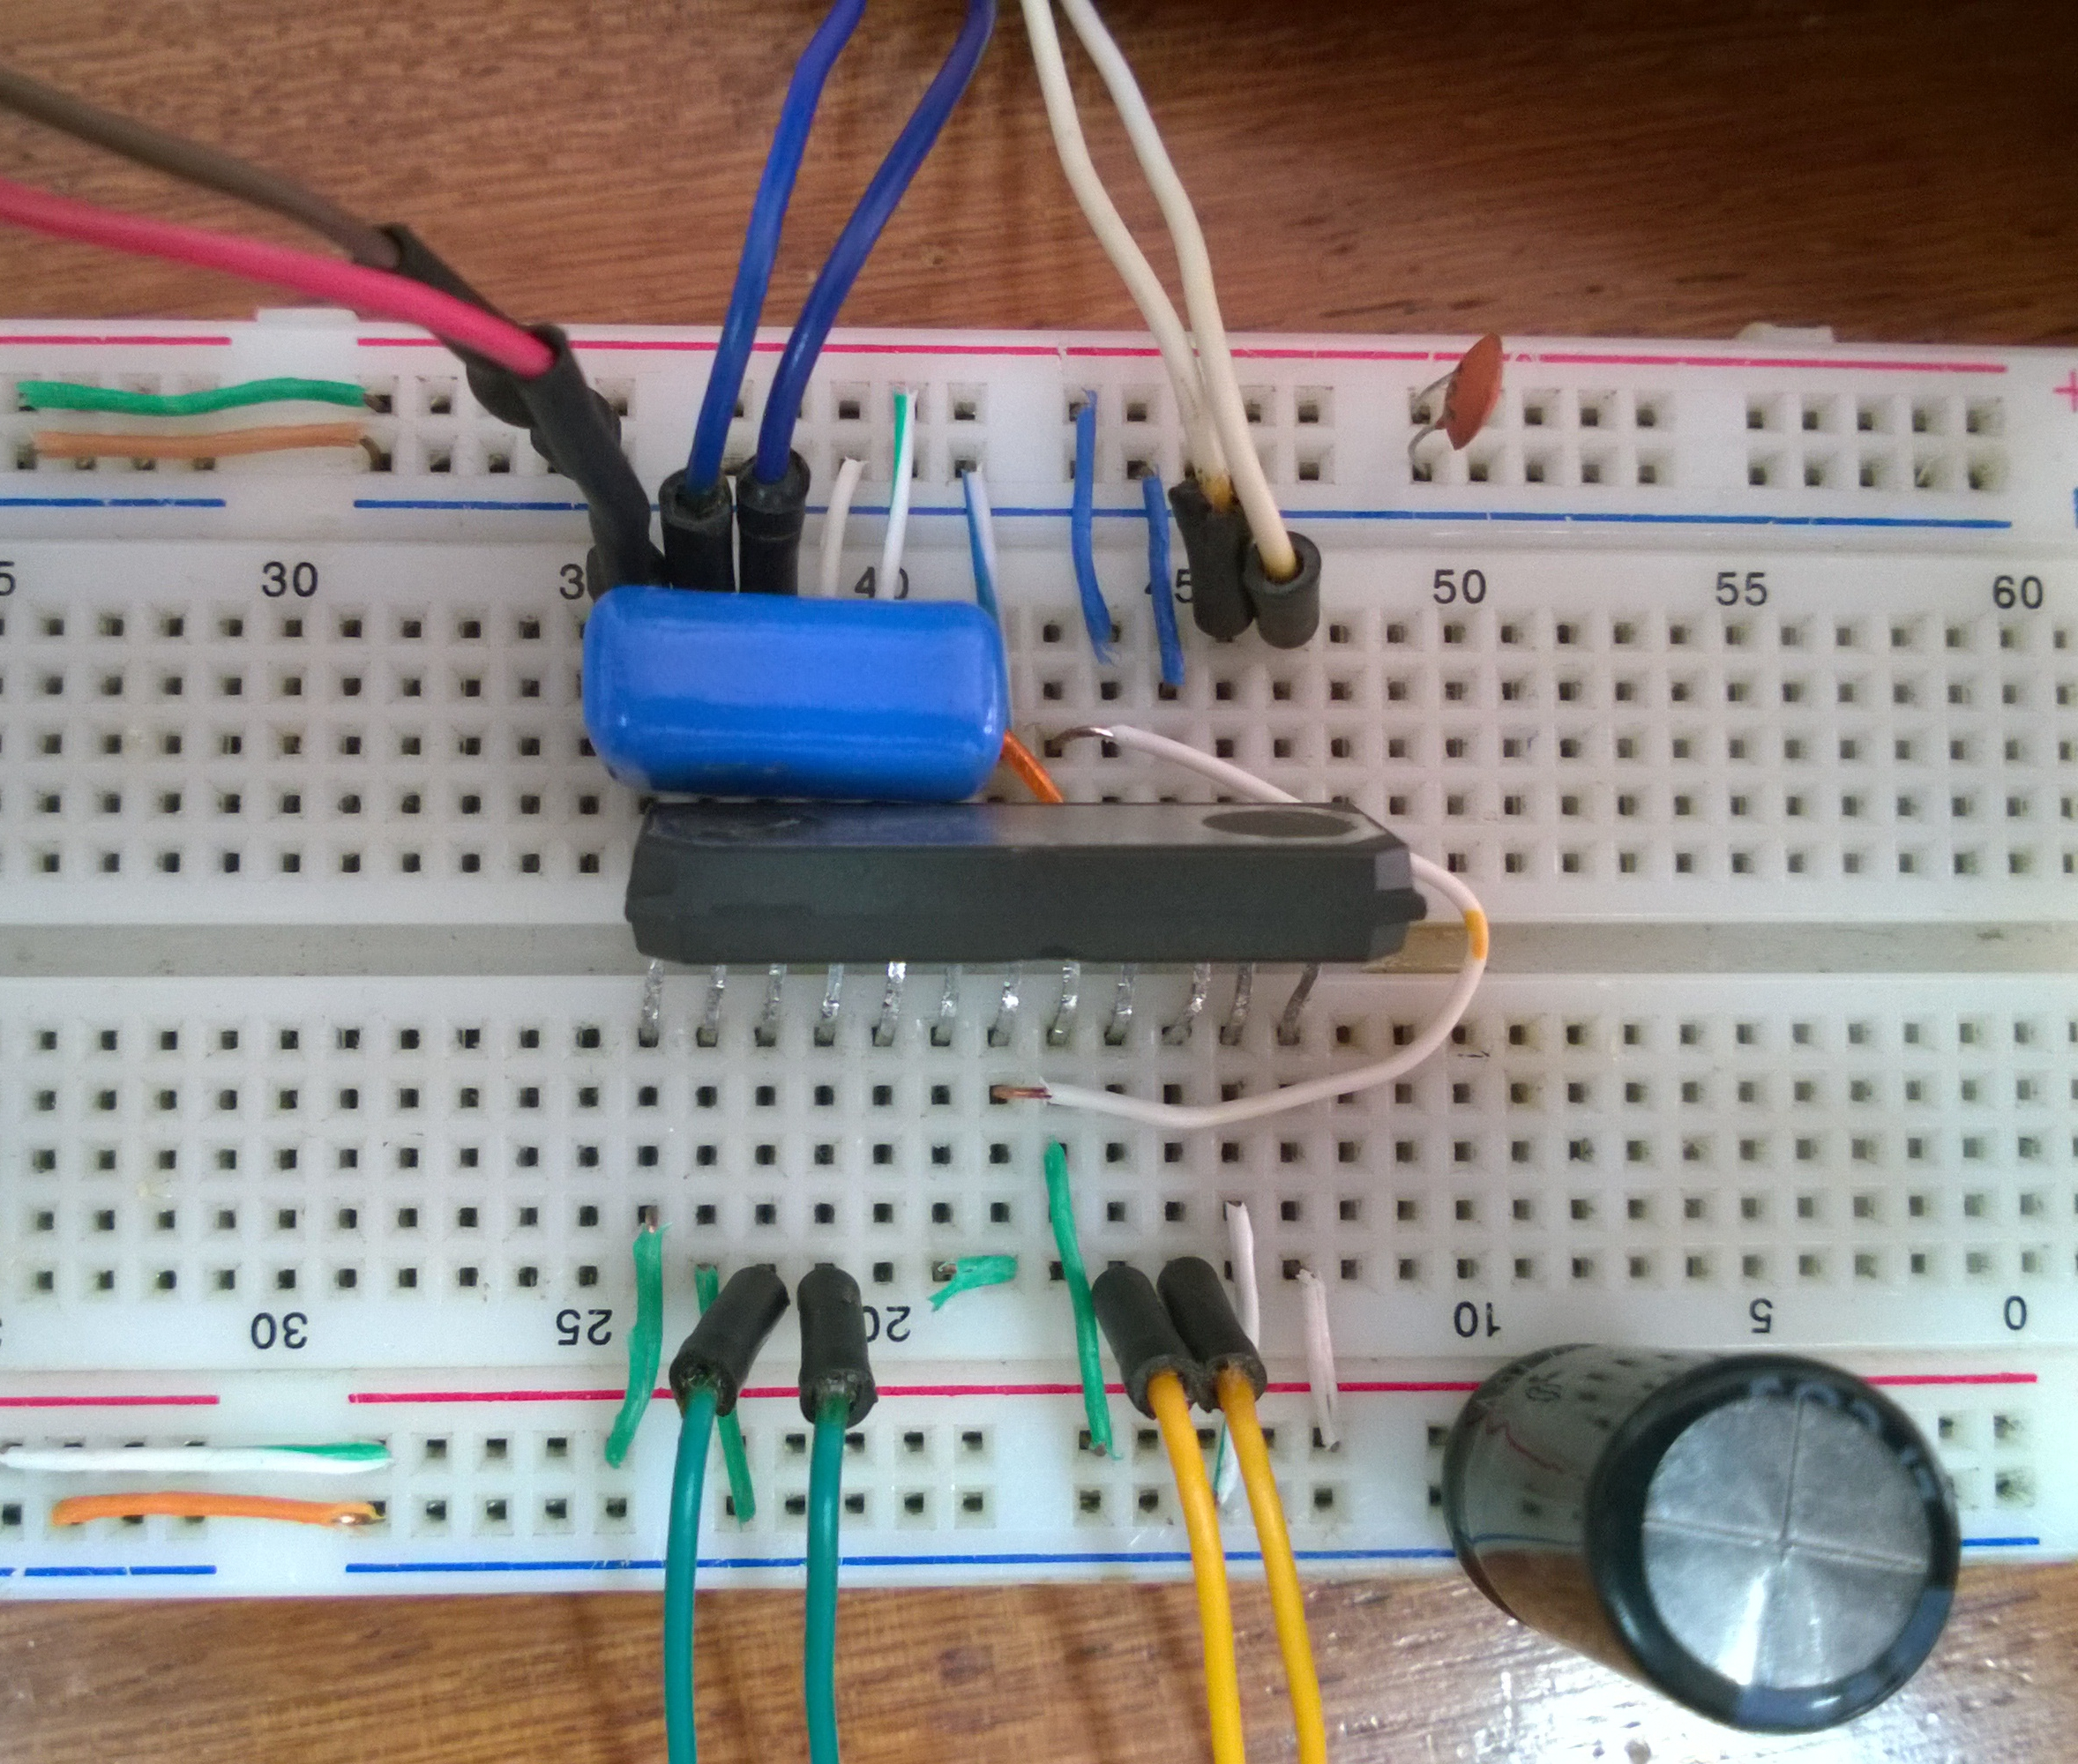
\includegraphics[width=0.7\textwidth]{figuras/Sistema_som_prot}
    \caption{Circuito amplificador de som montado na protoboard}
    \label{fig:Sistema_som_prot}
\end{figure}

\subsection{Sistema de Sensoriamento}

O projeto exige duas medidas para garantir seu bom funcionamento: a temperatura interna do recipiente dos picolés em resfriamento e um detector de presença para atender um possível cliente e economizar energia.

Os sensores escolhidos são populares e amplamente utilizados em projetos com Arduino. Diante disso, várias bibliotecas foram criadas com grandes históricos de aprimoramento e, por isso, o Arduino foi escolhido para recolher e tratar os dados dos sensores, os quais devem ser enviados ao controlador geral (Raspberry Pi).

Para a medida de temperatura, é utilizado o sensor DS18B20 à prova d'água fabricado pela Maxim Integrated, sendo ideal para medidas em temperaturas na faixa de -10º C a 85º C com precisão de 0.5º C, o qual é suficiente para o projeto.

Para a detecção de presença, é utilizado o sensor HC-SR04, o qual mede distância por meio de sinais ultrassônicos, sendo utilizado para detectar clientes nos quatro lados do recipiente de vendas (utilizando assim, quatro sensores). O sensor possui um alcance máximo de 4 metros e mínimo de 2 centímetros, sendo ideal para a detecção de usuários que se aproximam da máquina de vendas \cite{mq3}. A ideia de detectar uma pessoa por perto é economizar energia desligando-se o sistema visual quando não há ninguém por perto, além de dar boas vindas ao cliente com um assistente de voz, dando rápidas instruções de como efetuar uma compra.

\subsubsection{Implementação}

Para a implementação dos sensores, utilizou-se plataforma UART do Arduino UNO. Para o sensor de temperatura, utilizou-se a seguinte montagem (criado com o software Fritzing):

Para o sensor de temperatura, não se pode ligar o fio de dados diretamente no Arduino, pois pontos flutuantes podem ocorrer. Dessa forma, é necessário utilizar um resistor de pullup como mostrado na figura \ref{fritzing_temp}. Para o código, foi utilizado as bibliotecas OneWire.h, o qual é responsável por realizar o protocolo de comunicação serial de um fio (simplex, o sensor apenas envia dados) e DallasTemperature.h o qual recebe e trata os dados, fazendo a conversão para graus Celsius.

Já, o princípio de funcionamento dos sensores ultrassônicos está baseado na emissão de uma onda sonora de alta frequência, e na medição do tempo levado para a recepção do eco produzido quando esta onda se choca com um objeto capaz de refletir o som, ou seja, é capaz de medir distâncias emitindo uma onda sonora que rebate em um obstáculo e é detectada de volta. A detecção do eco incidente, depende de sua intensidade e esta da distância entre o objeto e o sensor ultrassônico. Os sensores ultrassônicos funcionam medindo o tempo de propagação do eco. Ou seja, o intervalo de tempo medido entre o impulso sonoro emitido e o eco do
mesmo conforme a figura abaixo.

% \begin{figure}[H]
% \centering
% 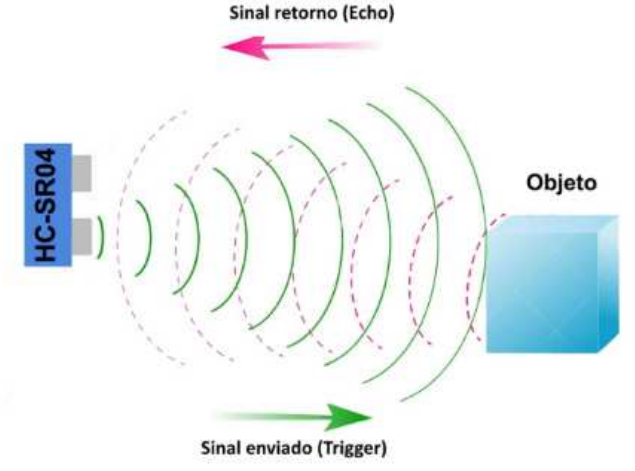
\includegraphics[width=0.4\textwidth]{figuras/sensor_ultrasom}
%  \caption{Sinais de Envio e Retorno do Sensor Ultrassônico}
% \label{fig:sensor_ultrasom}
% \end{figure}

O sensor possui dois pinos de dados: o pino ECHO que fica em nível alto caso a onda seja detectada e nível baixo caso contrário. Com o pino TRIGGER, é possível emitir uma onda sonora com um pulso. Como visto na figura abaixo. 

% \begin{figure}[H]
% \centering
% 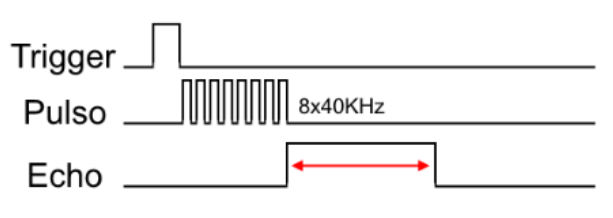
\includegraphics[width=0.4\textwidth]{figuras/trigger}
%  \caption{Pulsos de Envio e Retorno do Sensor Ultrassônico}
% \label{fig:trigger}
% \end{figure}

Logo, é possível medir o tempo levado para este processo e, consequentemente, medir a distância sabendo-se a velocidade do som. Foi utilizado a biblioteca Ultrasonic.h que já realiza essas conversões.

\subsubsection{Testes}

Para o sensor de temperatura, utilizou-se a seguinte montagem (criado com o software Fritzing):

\begin{figure}[H]
	\centering
    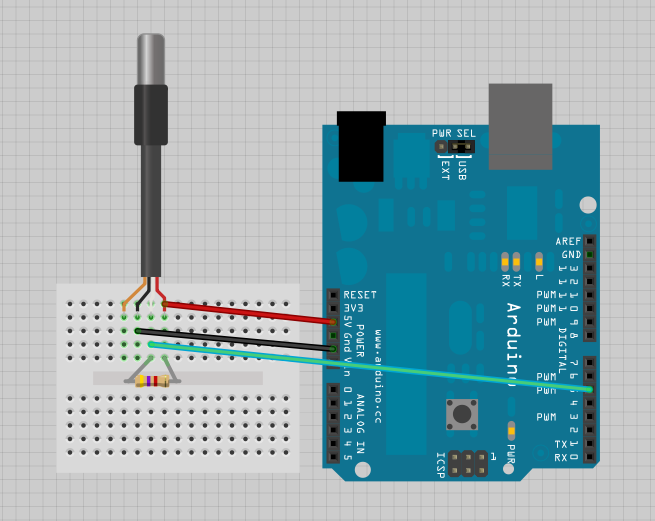
\includegraphics[width=0.8\textwidth]{figuras/fritzing_temp}
    \caption{Montagem para o sensor de temperatura}
    \label{fig:fritzing_temp}
\end{figure}

O sensor funcionou com sucesso. Um teste realizado foi colocá-lo num recipiente com água e gelo. A temperatura medida no monitor serial do Arduino foi de 0º C, o qual é o esperado.

Para o sensor de presença, utilizou-se a seguinte montagem (criado com o software Fritzing):

\begin{figure}[H]
	\centering
    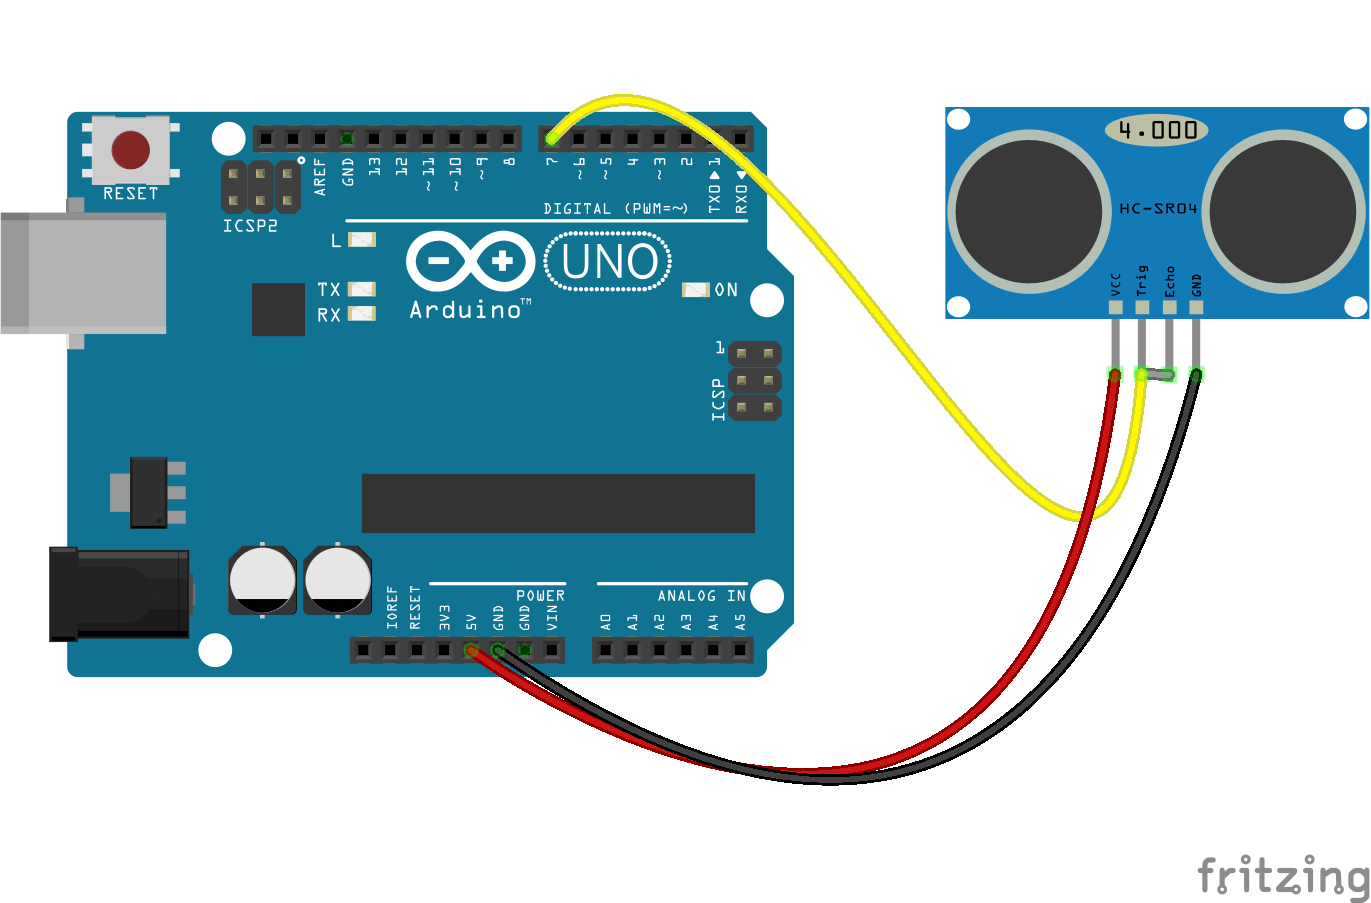
\includegraphics[width=0.8\textwidth]{figuras/fritzing_presenca}
    \caption{Montagem para o sensor de presença}
    \label{fig:fritzing_presenca}
\end{figure}

O sensor funcionou com sucesso. Vários testes foram realizados com diversos obstáculos. A distância aferida possuiu erro máximo de 5 cm para mais ou menos, o que é aceitável para sua aplicação.

\subsection{Sistema dos Motores}
Os picolés serão entregues por meio de um sistemas de molas similar a de máquinas de venda. Um picolé situado no meio de uma mola faz um movimento linear quando este se rotaciona, como ilustra a imagem \ref{fig:sistema_molas} a seguir:

\begin{figure}[H]
	\centering
    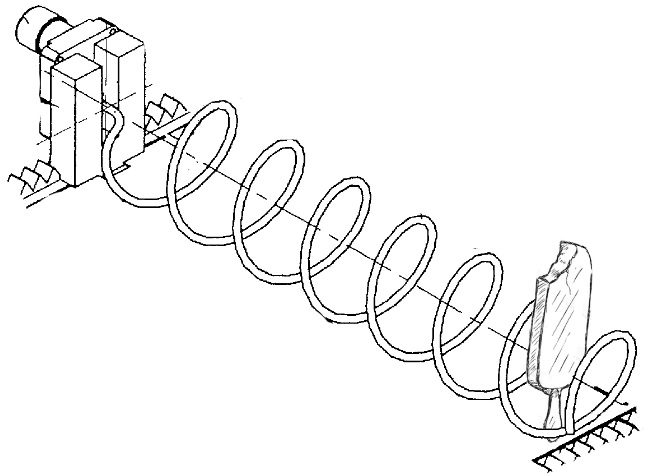
\includegraphics[width=0.8\textwidth]{figuras/sistema_molas}
    \caption{Sistema de molas capaz de movimentar os picolés}
    \label{fig:sistema_molas}
\end{figure}

Logo, é necessário inserir um motor ao final de cada mola e fazer o controle do giro para que os picolés caiam conforme o pedido do cliente. Para que se realizasse este objetivo, a proposta inicial se tratava da utilização de um motor do tipo servomotor, uma vez que possui torque suficiente para movimentar a longa fileira de picolés situados na mola com uma precisão de uma volta (360\degree por venda), além da facilidade de controle com apenas um fio. Contudo, os servomotores adquiridos não giravam continuamente, pois possuíam um limite de uma revolução completa. Ao realizar uma modificação retirando-se a trava, o servomotor perdeu precisão e bastante torque. A compra de servomotores de giro contínuo torna-se inviável para o projeto devido ao seu alto custo. Devido a esses problemas, a nova escolha se trata de um motor encontrado em sucata. Este é um motor de passos TAMAGAWA SEIKIM do tipo TS3103N145, com 200 passos por revolução, torque de 6 Kgfcm e alimentação de 12V DC. Estes dados foram retirados na etiqueta do próprio motor, já que seu Datasheet não foi encontrado por ser muito antigo.

Sabe-se que o motor de passos necessita de um driver e, para isso, montou-se o drive de controle constituído por resistores de 220 Ohms, transístores TIP41C e diodos 1N4007. O circuito do driver funciona de tal forma que, quando um nível de tensão da saída do Arduino (pinos 8, 9, 10 e 11) passa de nível lógico para nível lógico alto, a junção \textit{VBE} do transistor bipolar é diretamente polarizada, causando um fluxo de corrente no terminal coletor do mesmo. O transistor então funciona operando como chave eletrônica (regiões de corte e saturação), quando é a junção base-emissor é diretamente polarizada, é aplicado uma diferença de potencial na bobina do motor e o rotor é movimentado, e assim sucessivamente para a realização dos passos desejados.

O esquemático desse drive (para cada motor) é apresentado na figura \ref{fig:motor1}:

% \begin{figure}[H]
% \centering
% 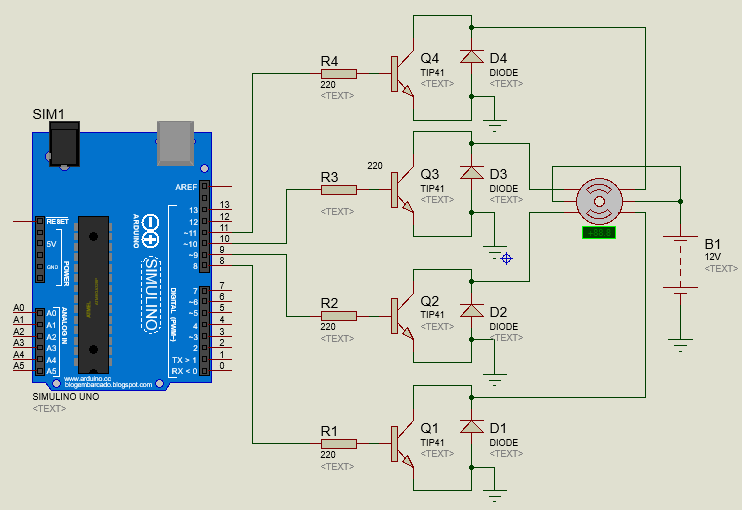
\includegraphics[width=0.4\textwidth]{figuras/motor1}
%  \caption{Esquemático do Driver realizado para o motor de Passos}
% \label{fig:motor1}
% \end{figure}

O motor de passos TAMAGAWA SEIKIM do tipo TS3103N145 possui saída com seis terminais, os quais foram identificados com utilização do multímetro para correta conexão das bobinas no driver. Como a implementação proposta requer o funcionamento de quatro motores (para o controle de quatro molas), seria necessária a utilização de 16 pinos do microcontrolador (tendo em vista que dois terminais de cada motor são terminais comuns). Para solucionar esse problema, um circuito foi simulado e implementado para demultiplexar as entradas para as quatro saídas. Foram utilizados dois CI's 74HC139 (4 demux 1x4). A seleção de qual motor rotacionar é definida pelo código dependendo do sabor escolhido pelo cliente. 

O esquemático utilizado em simulação do circuito completo de controle do motor, incluindo microcontrolador, circuito demultiplexador, drivers e motores, é mostrado na figura \ref{fig:motor_completo} a seguir:

% \begin{figure}[H]
% \centering
% 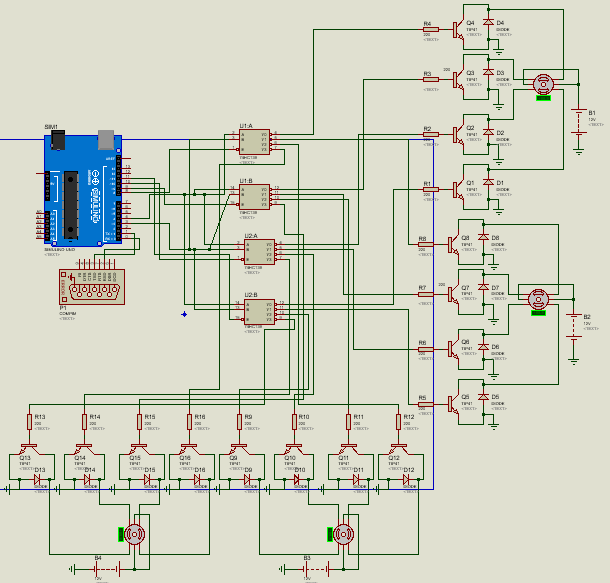
\includegraphics[width=0.4\textwidth]{figuras/motor_completo}
%  \caption{Esquemático do circuito completo de controle dos motores de passos}
% \label{fig:motor_completo}
% \end{figure}

\subsubsection{Implementação}

Para implementação dos motores de passos juntos, foi montado o circuito em protoboard e utilizou-se a plataforma UART do Arduino UNO, de forma que a entrada é o sabor escolhido pelo cliente e o controlador realiza a revolução no motor da mola desejada para aquele determinado sabor. Para realizar a revolução no eixo do motor, foi utilizada a biblioteca padrão do Arduino UNO para motores de passos, a \textit{Stepper.h}. Sua implementação em software requer selecionar a velocidade de rotação em RPM,

O código funciona da seguinte forma: um código de sabor é escolhido pelo cliente. O programa então entra em uma função condicional \textit{switch case} de quatro casos (quatro sabores) e em cada um dos casos, um dos motores será acionado e, caso o código seja incorreto, um novo código de sabor é requisitado. O que acontece, de fato, é que o mesmo sinal para revolução do motor sai em todos os casos pelos quatro pinos (pinos 8, 9, 10 e 11), e é função do circuito demultiplexador direcionar essas quatro saídas para o motor desejado, através da variável de seleção de 2 bits (quatro casos) escolhida nos pinos 3 e 4. 

\subsubsection{Testes}

O teste do circuito controlador dos motores de passos foi então feito. O sistema então responde de forma correta e eficiente. 

A montagem em protoboard do circuito controlador dos motores pode ser mostrado na figura \ref{fig:circuito_motor_montado}

% \begin{figure}[H]
% \centering
% 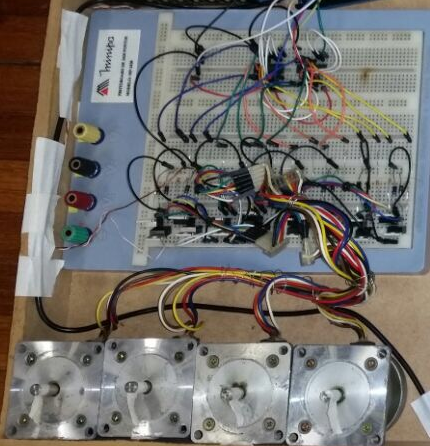
\includegraphics[width=0.4\textwidth]{figuras/circuito_motor_montado}
%  \caption{Circuito completo de controle dos motores de passos em protoboard}
% \label{fig:circuito_motor_montado}
% \end{figure}




\subsection{Sistema do Acionamento do Compressor}

A refrigeração do recipiente vai ser feita por meio de um compressor. Mantê-lo ligado o tempo todo não é viável devido à limitação da demanda energética. Para isso, será feito um controle de acionamento do compressor de acordo com os dados enviados pelo sensor de temperatura. Para ligar e desligar o compressor, será utilizado um módulo relé JQC-3F. O relé é um componente eletromecânico capaz de realizar a função de uma espécie de chave selecionadora. Por meio dela, é possível fazer o acionamento de sistemas de alta potência com um controlador sem danificá-lo e puxar muita corrente.

Como o controlador utilizado para adquirir dados do sensor de temperatura é o Arduino, convém utilizá-lo também para fazer o acionamento do relé. Para isso, convencionou-se uma faixa de temperaturas entre -2º C e 2º C. Quando a temperatura atingida for menor que -2º C, o compressor é desligado. Quando a temperatura atingida for maior que 2º C, o compressor é religado.

\subsection{Sistema de Interface Visual}

A ideia central da máquina de vendas é a sua capacidade de realizar vendas de picolé pelo aplicativo de celular sem um vendedor presente. Portanto, convém utilizar um sistema visual na qual poderá mostrar informações ao usuário tais como:

\begin{itemize}
  \item O estoque dos sabores dos picolés;
  \item Um rápido tutorial de como obter e utilizar o aplicativo;
  \item Caso o picolé seja vendido, informar ao usuário sua retirada;
  \item Fazer propaganda do produto.
\end{itemize}

Para isso, há uma tela LCD de 7 polegadas embutido na máquina de vendas de fácil visualização para os clientes. Essa tela vem com um driver que recebe um sinal de vídeo por HDMI proveniente do Raspberry Pi. Para economizar energia, a tela será acionada quando uma pessoa for detectada pelo sensor de presença.

\subsection{Bancada de Testes para os Sistemas Eletrônicos}

Essa subseção apresenta o protótipo de teste para os sistemas propostos neste relatório. Na bancada de testes, inseriu-se todos os sistemas eletrônicos propostos para validação, implementação e testes, como mostrado na figura  \ref{fig:bancada_teste_eletronica}.

% \begin{figure}[H]
% \centering
% 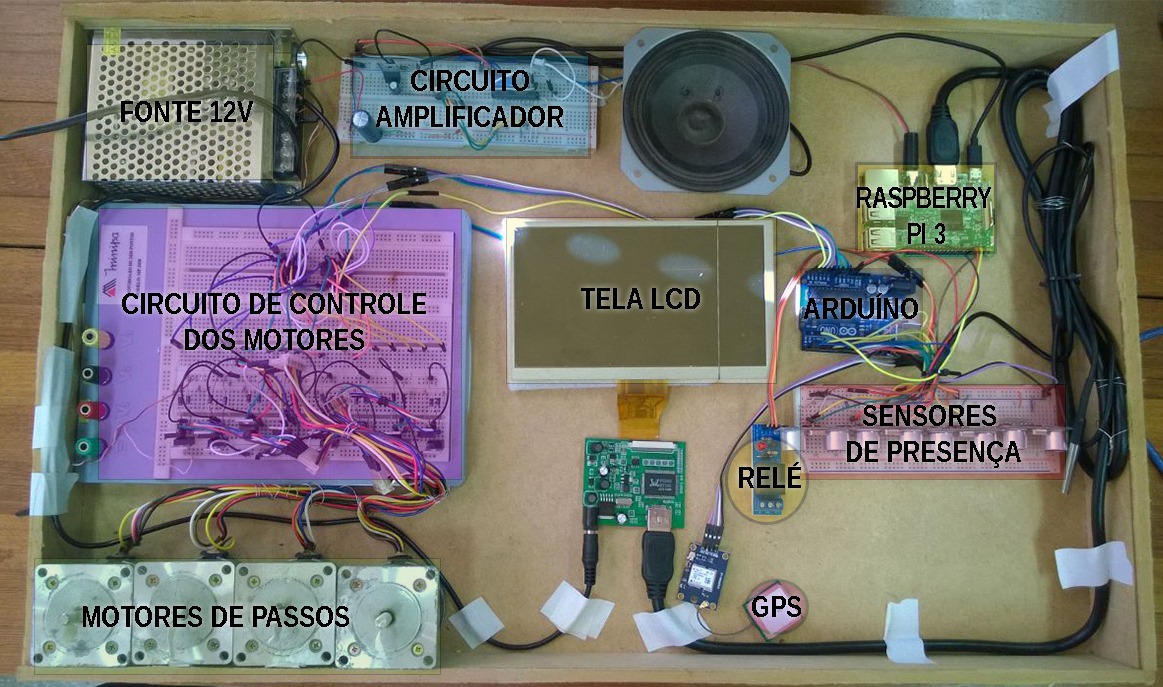
\includegraphics[width=0.4\textwidth]{figuras/bancada_teste_eletronica}
%  \caption{Bancada de Testes para os Sistemas Eletrônicos}
% \label{fig:bancada_teste_eletronica}
% \end{figure}

A imagem da tela do monitor serial (UART) do Arduino pode ser mostrada na figura \ref{fig:serialmonitor_motor}

% \begin{figure}[H]
% \centering
% 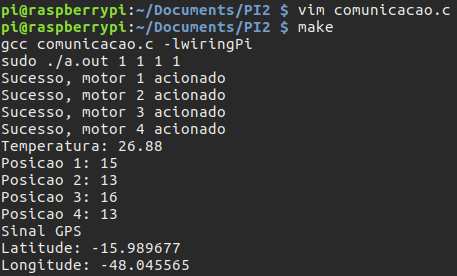
\includegraphics[width=0.4\textwidth]{figuras/serial_bancada}
%  \caption{Monitor serial para sistema eletrônico integrado}
% \label{fig:serial_bancada}
% \end{figure}

A bancada de testes é um instrumento para validação mais precisa antes da implementação dos sistemas em uma PCB mais robusta, uma vez que, todos eles, devem ser testados antes do protótipo final que será entregue no Ponto de Controle 3.

\subsection{Integração de Todos os Sistemas Eletrônicos}
 Esta seção apresenta a integração dos sistemas e, por consequência, o sistema de controle do produto. Para isso, de forma sucinta,  utilizou-se o Raspberry Pi 3 e o Arduino UNO.

\subsubsection{Raspberry Pi 3}

O controlador escolhido para integrar todos os sistemas é o Raspberry Pi 3, o qual é um computador com um processador ARM de 1.2 GHz 64 bit, 1 Gb de RAM e Bluetooth. É um controlador popular, uma vez que, é de fácil intuição a sua aprendizagem. Possui capacidade de embutir um sistema operacional como o Linux, o que pode tornar o sistema mais estável e com menos memória de uso. Sua escolha se justifica pelo fato de conter todos os requisitos exigidos para cada sistema, tais como:

\begin{itemize}
  \item Possui entradas e saídas digitais as quais podem ser usadas para controle dos sistemas GPRS;
  \item Possui saída de áudio para o sistema de som;
  \item Possui saída de vídeo para o sistema de interface com o usuário;
  \item Possui entradas TX e RX que permitem a comunicação serial com o outro microcontrolador, no caso específico, o Arduino.
\end{itemize}

\subsubsection{Arduino}
O Arduino é uma plataforma eletrônica de hardware livre e de placa única, integrada a um microcontrolador ATMEL AVR com suporte de entrada/saída embutido, é constituído de uma linguagem de programação padrão e de fácil utilização, de origem em Wiring, e é, basicamente, C/C++. Este microcontrolador tem uma plataforma UART (Universal Asynchronous Receiver/Transmitter), a qual é um bloco de circuitos
responsável pela implementação da comunicação serial. De forma geral, o UART atua como um mediador entre interfaces paralelas e em série. Como demonstrada na figura a seguir.

% \begin{figure}[H]
% \centering
% 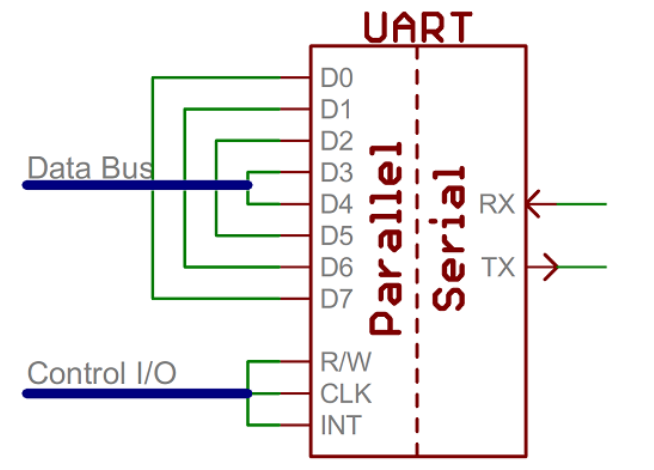
\includegraphics[width=0.4\textwidth]{figuras/uart}
%  \caption{ Modelo simplificador da Plataforma UART}
% \label{fig:uart}
% \end{figure}

Como pode ser visto na figura, uma das extremidades do UART é um barramento de oito linhas de dados e alguns pinos de controle, a outra é formada pelos fios de transmissão e recepção em série (TX e RX). Este microcontrolador por ser acessível financeiramente e também de fácil implementação, além de reter diversas bibliotecas de uso livre, o que abrange e facilita a execução do projeto aqui apresentado.

O Arduino foi utilizado para controlar e tratar sinais dos sistemas de sensoriamento, localização e acionamento do compressor. Para isso, é necessário juntar todos em um controlador Arduino apenas e adaptar o código para isso. Primeiramente, foi feito a análise da quantidade de pinos que serão utilizados:

\begin{table}[H]
\centering
\caption{Quantidade de pinos utilizados para ligar no Arduino}
\label{pinos_arduino}
\begin{tabular}{|l|c|c|}
\hline
\multicolumn{1}{|c|}{\textbf{Dispositivo}} & \multicolumn{1}{l|}{\textbf{Quantidade}} & \multicolumn{1}{l|}{\textbf{Pinos}} \\ \hline
Sensor de temperatura                      & 1                                        & 1                                   \\ \hline
Sensor de presença                         & 4                                        & 8                                   \\ \hline
Módulo Relé                                & 1                                        & 1                                   \\ \hline
Módulo GPS                                 & 1                                        & 2                                   \\ \hline
Comunicação Serial                         & 1                                        & 2                                   \\ \hline
Controle dos motores                       & 4                                        & 6                                   \\ \hline
\textbf{Total:}                            & -                                        & 20                                  \\ \hline
\end{tabular}
\end{table}

Como representado pela tabela acima, são necessários 20 pinos para ligar no Arduino. Logo, pode-se utilizar o Arduino UNO que dispõe de 20 pinos GPIO por meio do microcontrolador ATmega328, o qual pode ser removido da placa e acoplada numa placa de circuito impresso.

Um código foi implementado para integrar todos os dispositivos e funcionou com sucesso. A imagem a seguir é a saída do monitor serial para testar o protótipo:


\subsubsection{ Implementação do Sistema de Controle: Raspberry Pi 3 e Arduino UNO}

Após conhecer o computador de bordo e o microcontrolador utilizado, detalha-se aqui o processo de comunicação entre os mesmos. 
De forma concisa, a comunicação acontece entre os pinos  0 (RX) e 1 (TX) do Arduino Uno, e os pinos 10 (RX) no Raspberry Pi e 8 (TX) na GPIO. 

Entretanto, sabe-se que o Raspberry opera com 3.3V e necessita-se que o Arduíno opere a nível de sinal de 3.3V para envio do sinal \textit{Arduino (TX) -> Raspberry (RX)}, para que isso aconteça de forma eficiente, utiliza-se um divisor de tensão simples realizados com dois resistores de 10K. Apesar disso, a comunicação inversa, \textit{Raspberry (TX) -> Arduino (RX)}, pode ser direta, uma vez que o Arduíno opera em 5V e pode, descomplicadamente, interpretar o sinal do Raspberry. Ademais, acrescenta-se outro resistor de 10K para o pull-down do push-button A montagem do circuito para a comunicação pode ser visualizada na figura \ref{fig:comunicacao_rasp_arduino}.

% \begin{figure}[H]
% \centering
% 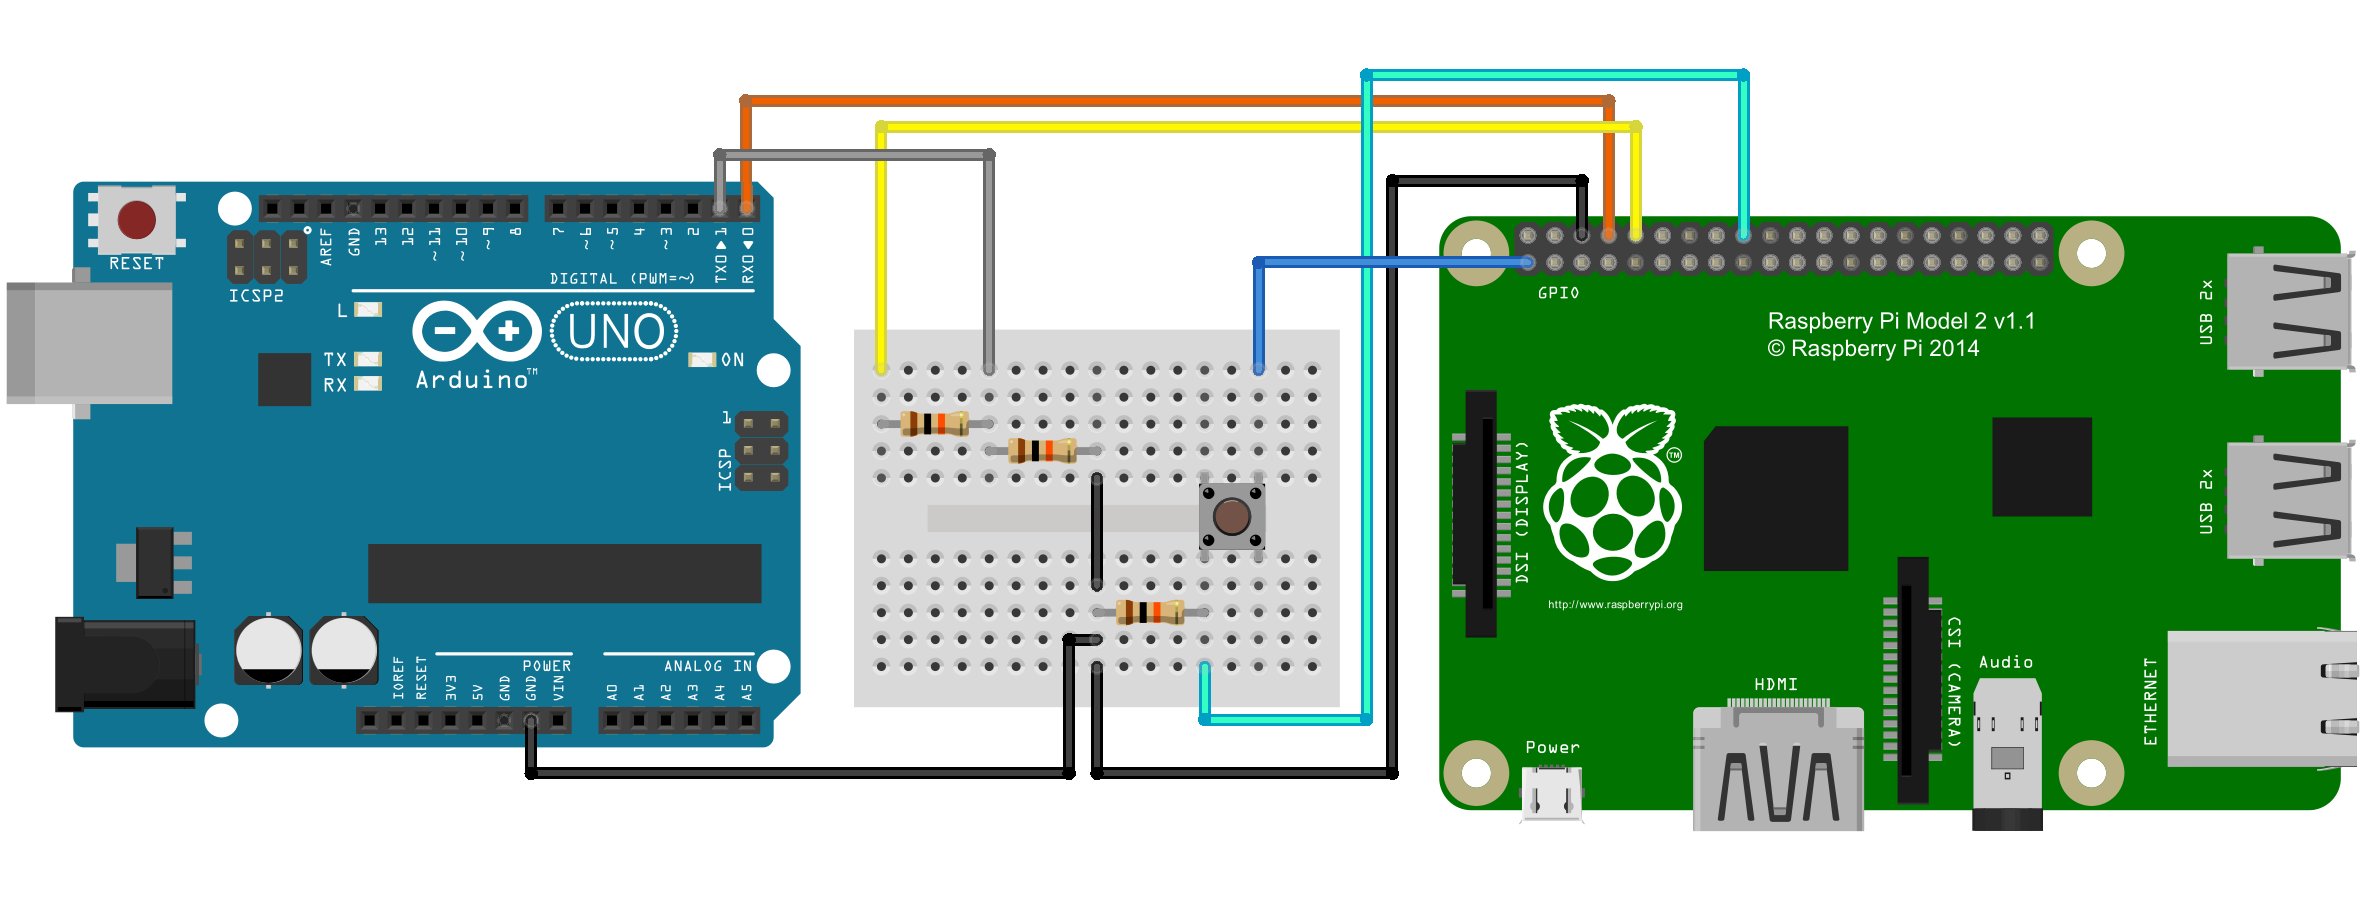
\includegraphics[width=0.4\textwidth]{figuras/comunicacao_rasp_arduino}
%  \caption{Esquemático para a Comunicação entre os controladores utilizados, realizados pela ferramente Fritzing}
% \label{fig:comunicacao_rasp_arduino}
% \end{figure}

%Além da execução do circuito, necessita-se configurar os ambientes antes mesmos de ligá-los. Para isso abriu-se no Raspberry a janela LXTerminal e editou-se o arquivo \textit{"/etc/inittab"}, acrescentando \textit{"#T0:23:respawn:/sbin/getty -L ttyAMA0 115200 vt100"}. Em seguida, o Raspberry foi reiniciado. 
Em seguida, verifica a comunicação entre os dois, onde, no Arduino é setado a velocidade de transmissão, configurada a porta serial, definida o pino do botão de entrada e o código do sistema. Após isso, a comunicação está pronta.


\subsection{Integração entre Software e Hardware}
A comunicação entre software e hardware será feita via internet e, para isso, é utilizado o módulo GSM GPRS SIM800L fabricado pela SIMCom. O módulo interligado à Raspberry PI 3 utiliza um cartão SIM para conexão com a internet e, dessa forma, a comunicação com o sistema de software é estabelecida.

\begin{figure}[H]
	\centering
    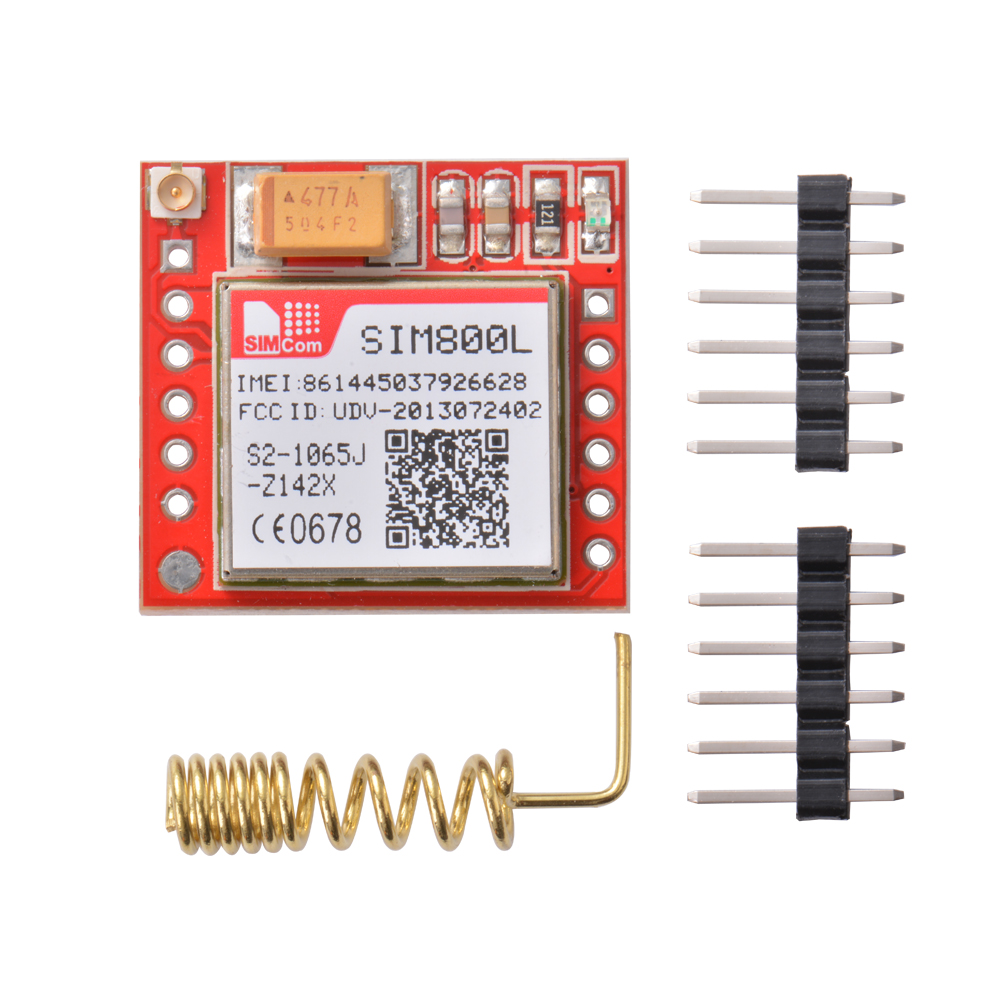
\includegraphics[scale=0.25]{figuras/modulo_gprs}
    \caption{Módulo GPRS SIM800L (SIMCom)}
    \label{fig:modulo_gprs}
\end{figure}

Esse sistema é responsável pelo funcionamento do produto final, uma vez que o servidor recebe informações de localização e segurança, e, também, o cliente compra via WebApp e o produto deve ser retirado em meio físico. O que torna necessário a utilização do GPRS e desta outra integração. 

\section{Solução de Estrutura}

\subsection{Propostas de possíveis soluções}
Como solução para a estrutura foram levantadas várias possibilidades de produtos para realizar a venda dos picolés, afim de escolher um conjunto que atenda às necessidades da indústria de picolés. À principio as opções eram:

\begin{itemize}
\item Triciclo com compartimento dianteiro
\item Triciclo com compartimento traseiro
\item Máquina de venda estática
\end{itemize}

\begin{figure}[H]
	\centering
    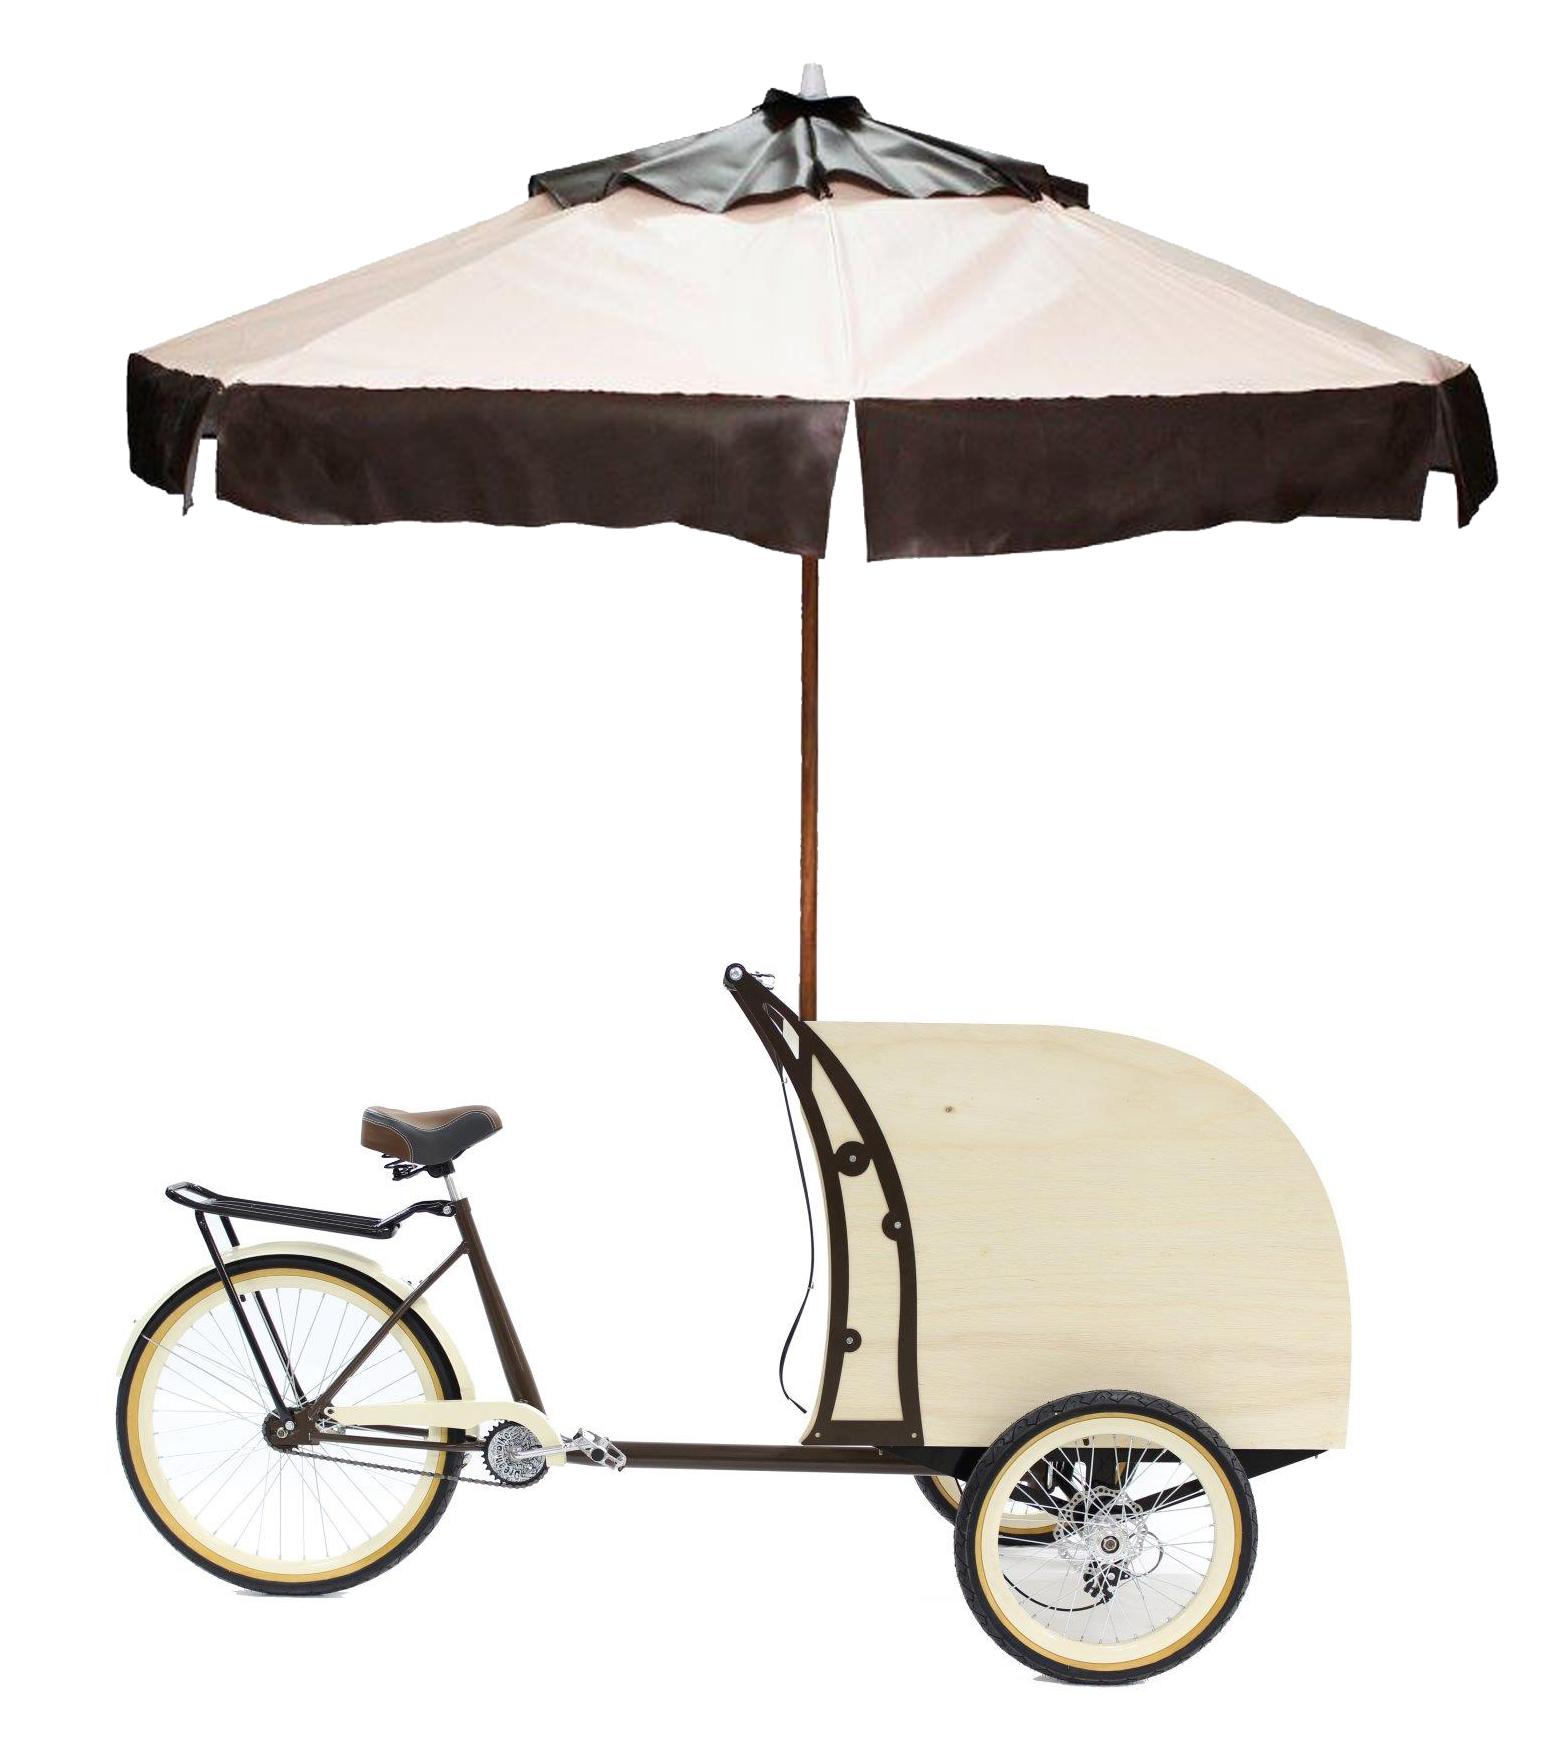
\includegraphics[width=0.6\textwidth]{figuras/exemplo2}
    \caption{Triciclo com Compartimento Dianteiro}
    \label{fig:exemplo2}
\end{figure}

\begin{figure}[H]
	\centering
    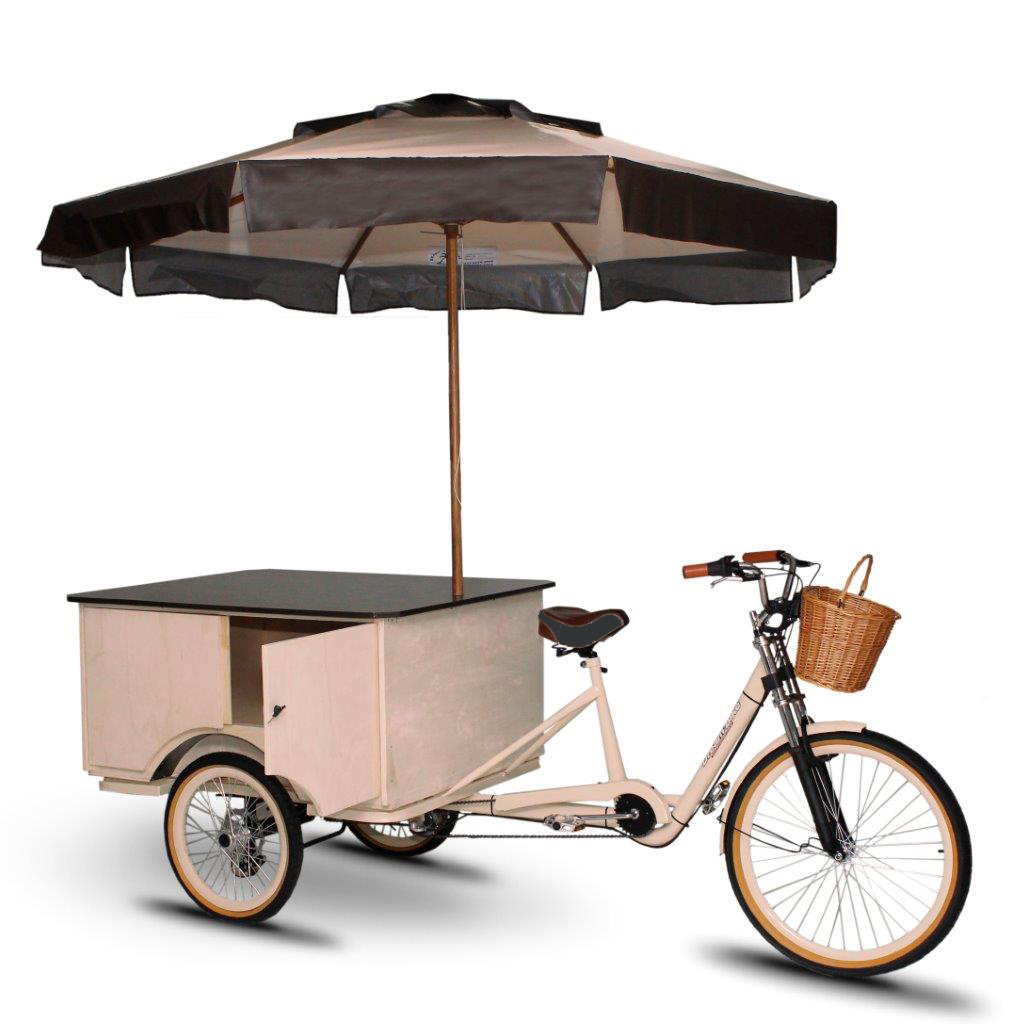
\includegraphics[width=0.6\textwidth]{figuras/exemplo}
    \caption{Triciclo com Compartimento Traseiro}
    \label{fig:exemplo}
\end{figure}

\begin{figure}[H]
	\centering
    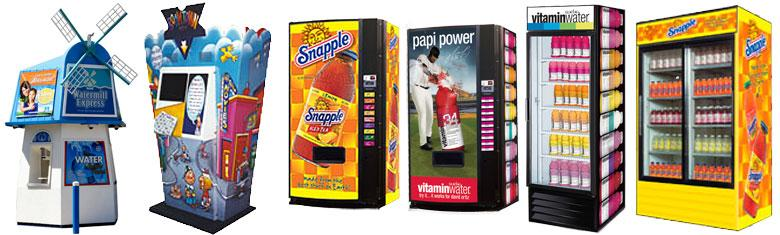
\includegraphics[width=0.6\textwidth]{figuras/machinewrapsheader}
    \caption{\textit{Vending Machine}}
    \label{fig:machinewrapsheader}
\end{figure}

Após consultoria com a empresa de sorvetes Saborizze®, não se tornou viável a utilização de triciclos no transporte da máquina de vendas automáticas devido a necessidade de um funcionário da empresa contratado apenas para conduzir o triciclo. Vendo isso, como solução de projeto de acordo com a aplicabilidade no mercado, foi escolhido como estrutura de projeto uma máquina de venda automática (\textit{vending machine}) que pode ser carregada por carro de transporte até o ponto de interesse pra ser realizada a venda dos picolés.


\subsection{Proposta acolhida para o projeto}

Como dito anteriormente, foi escolhido uma estrutura estática com acoplamento para um mecanismo de transporte. A construção desta estrutura escolhida pôde então ser subdividida da seguinte maneira:

 \begin{itemize}
\item Estrutura de suporte das placas solares

A estrutura para o suporte da placa solar ainda não foi construído devido ao fato da mesma não ter sido ainda integrada ao sistema.
\item Mecanismos para venda automatizada de picolé

O mecanismo para entrega dos picolés será composto por quatro espirais feitas em aço inox encaixadas dentro do freezer e controladas por motores de passo. Entre as espirais seram construídas paredes em policloreto de vinil (PVC) para manter os picolés alinhados. Ao girar a espiral, os picolés serão empurrados na direção de uma cavidade que foi feita no fundo do freezer, derrubando o picolé dentro de uma caixa que também possuirá isolamento térmico e será onde o cliente terá acesso ao produto.
\item Dimensionamento da estrutura 

Aferiu-se as massas de cada um dos elementos dos subsistemas da máquina. Com tais dados foi possível determinar o CG (centro de gravidade) da estrutura, de modo a averiguar a estabilidade da mesma. As coordenadas do CG podem estão destacadas na figura \ref{fig:cad_vista_lateral} em centímetros. Para obter informações mais detalhadas do dimensionamento da estrutura, vide anexo \label{app:visao_explodida}.

   \begin{figure}[H]
	\centering
    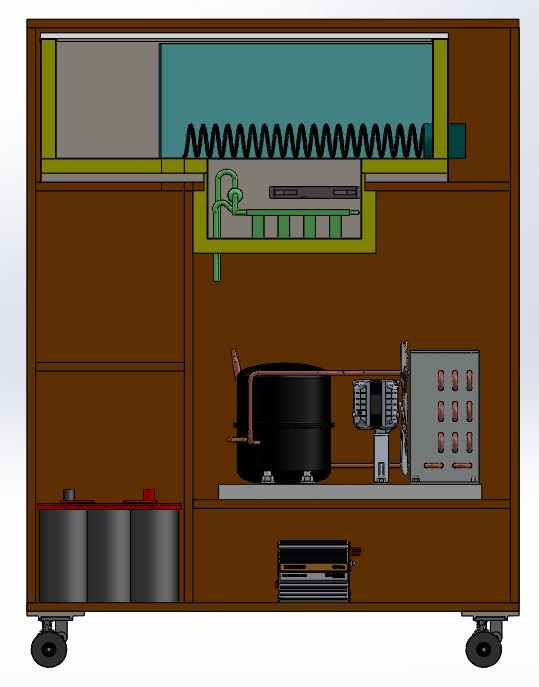
\includegraphics[width=0.8\textwidth]{figuras/cad_vista_lateral}
    \caption{Vista lateral em corte indicando o centro de massa [cm].}
    \label{fig:cad_vista_lateral}
\end{figure}


\item Compartimentos da máquina de vendas

A máquina de vendas possui três compartimentos principais que podem ser vistos na figura \ref{fig:cad_ZONAS}: compartimento para baterias e compressor (1), compartimento para os componentes eletrônicos (2), compartimento do freezer com isolamento térmico (3) e armazenamento temporário dos picolés (4).

%    \begin{figure}[H]
% 	\centering
%     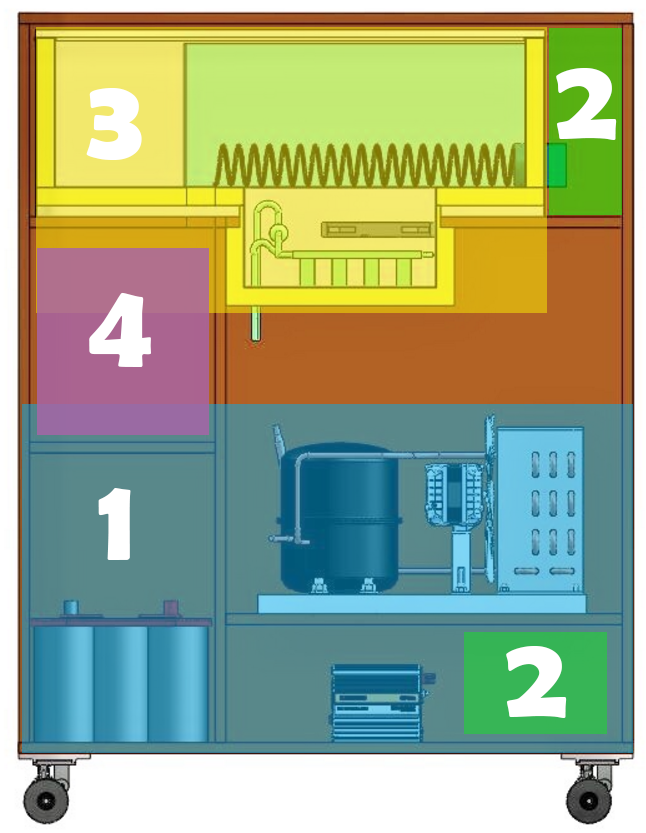
\includegraphics[width=0.4\textwidth]{figuras/cad_ZONAS}
%     \caption{Compartimentos dedicados.}
%     \label{fig:cad_ZONAS}
% \end{figure}

A porta superior foi construída e parte das prateleiras para o posicionamento dos subsistemas já foram montadas como pode ser observado na figura \ref{fig:armario_vista_isometrica}. O desenho técnico da estrutura completa encontra-se no anexo \ref{app:estante}.

% Atualizar a figura da estrutura de MDF

%    \begin{figure}[H]
% 	\centering
%     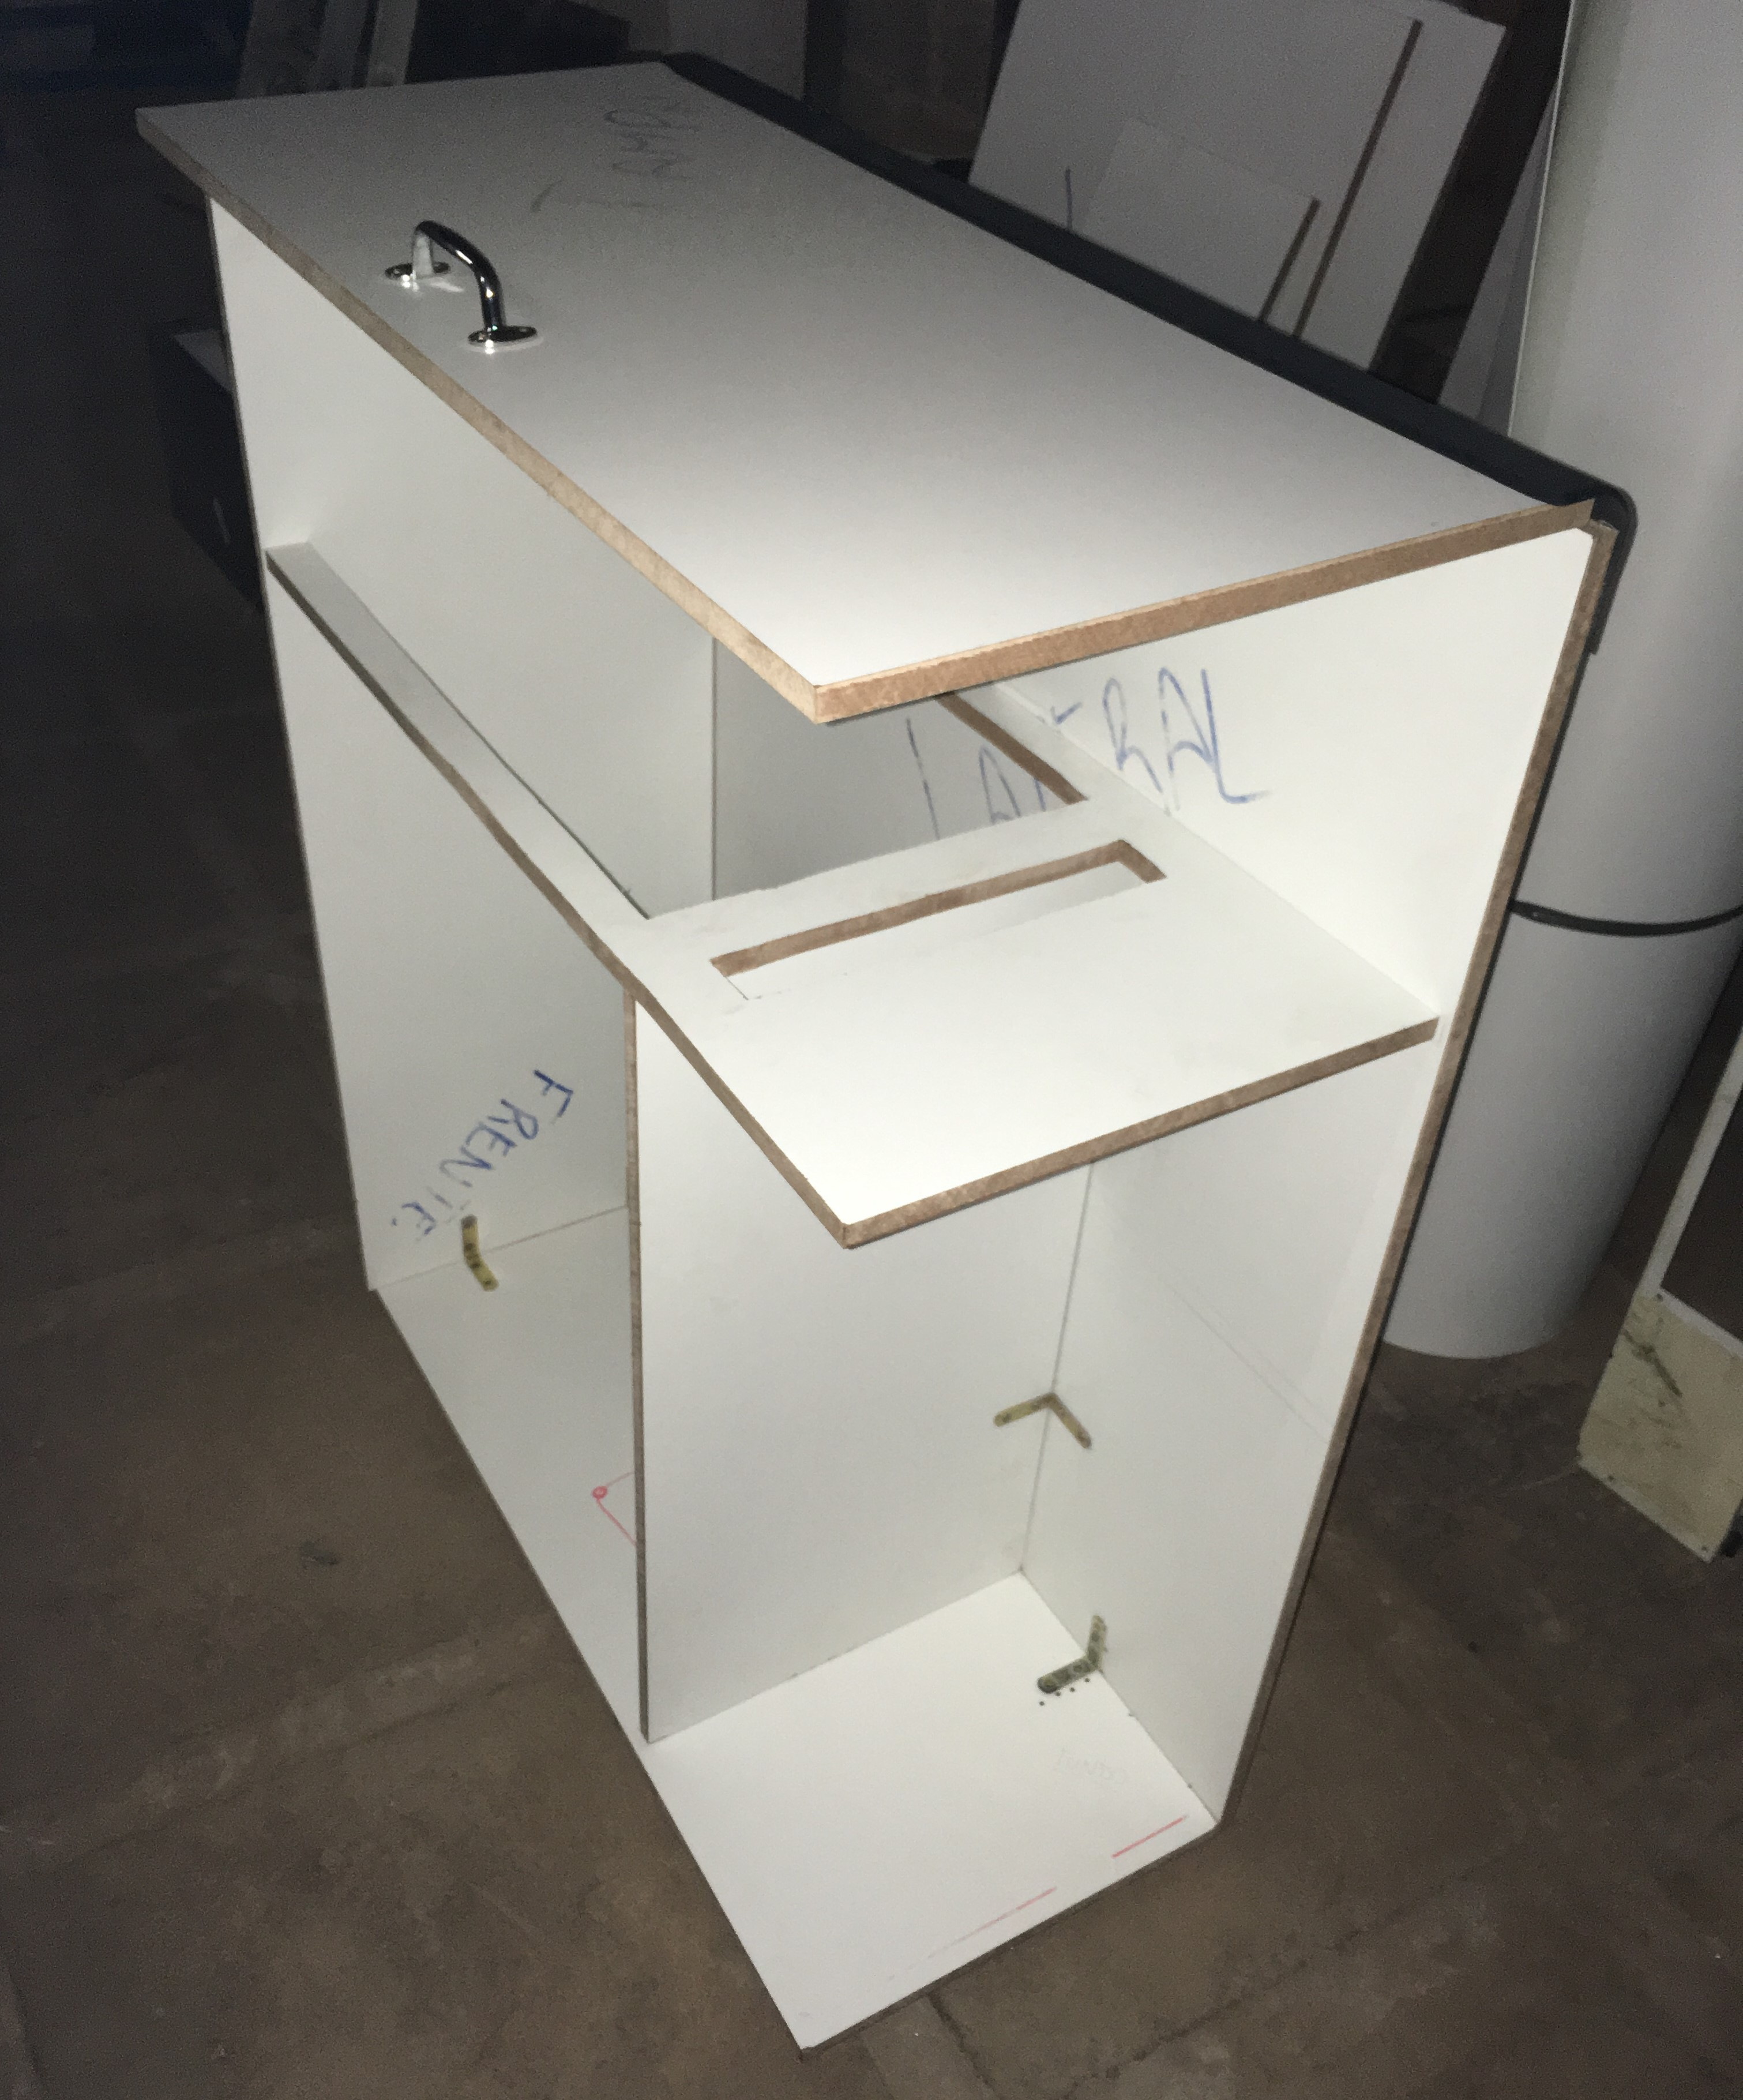
\includegraphics[width=0.4\textwidth]{figuras/armario_vista_isometrica}
%     \caption{Estrutura em MDF}
%     \label{fig:armario_vista_isometrica}
% \end{figure}

\item Freezer

O freezer foi adaptado a partir de uma estrutura doada (fig. \ref{fig:freezer}) onde será construído um isolamento térmico com placas de isopor e PVC.

% Figura antiga do freezer

%    \begin{figure}[H]
% 	\centering
%     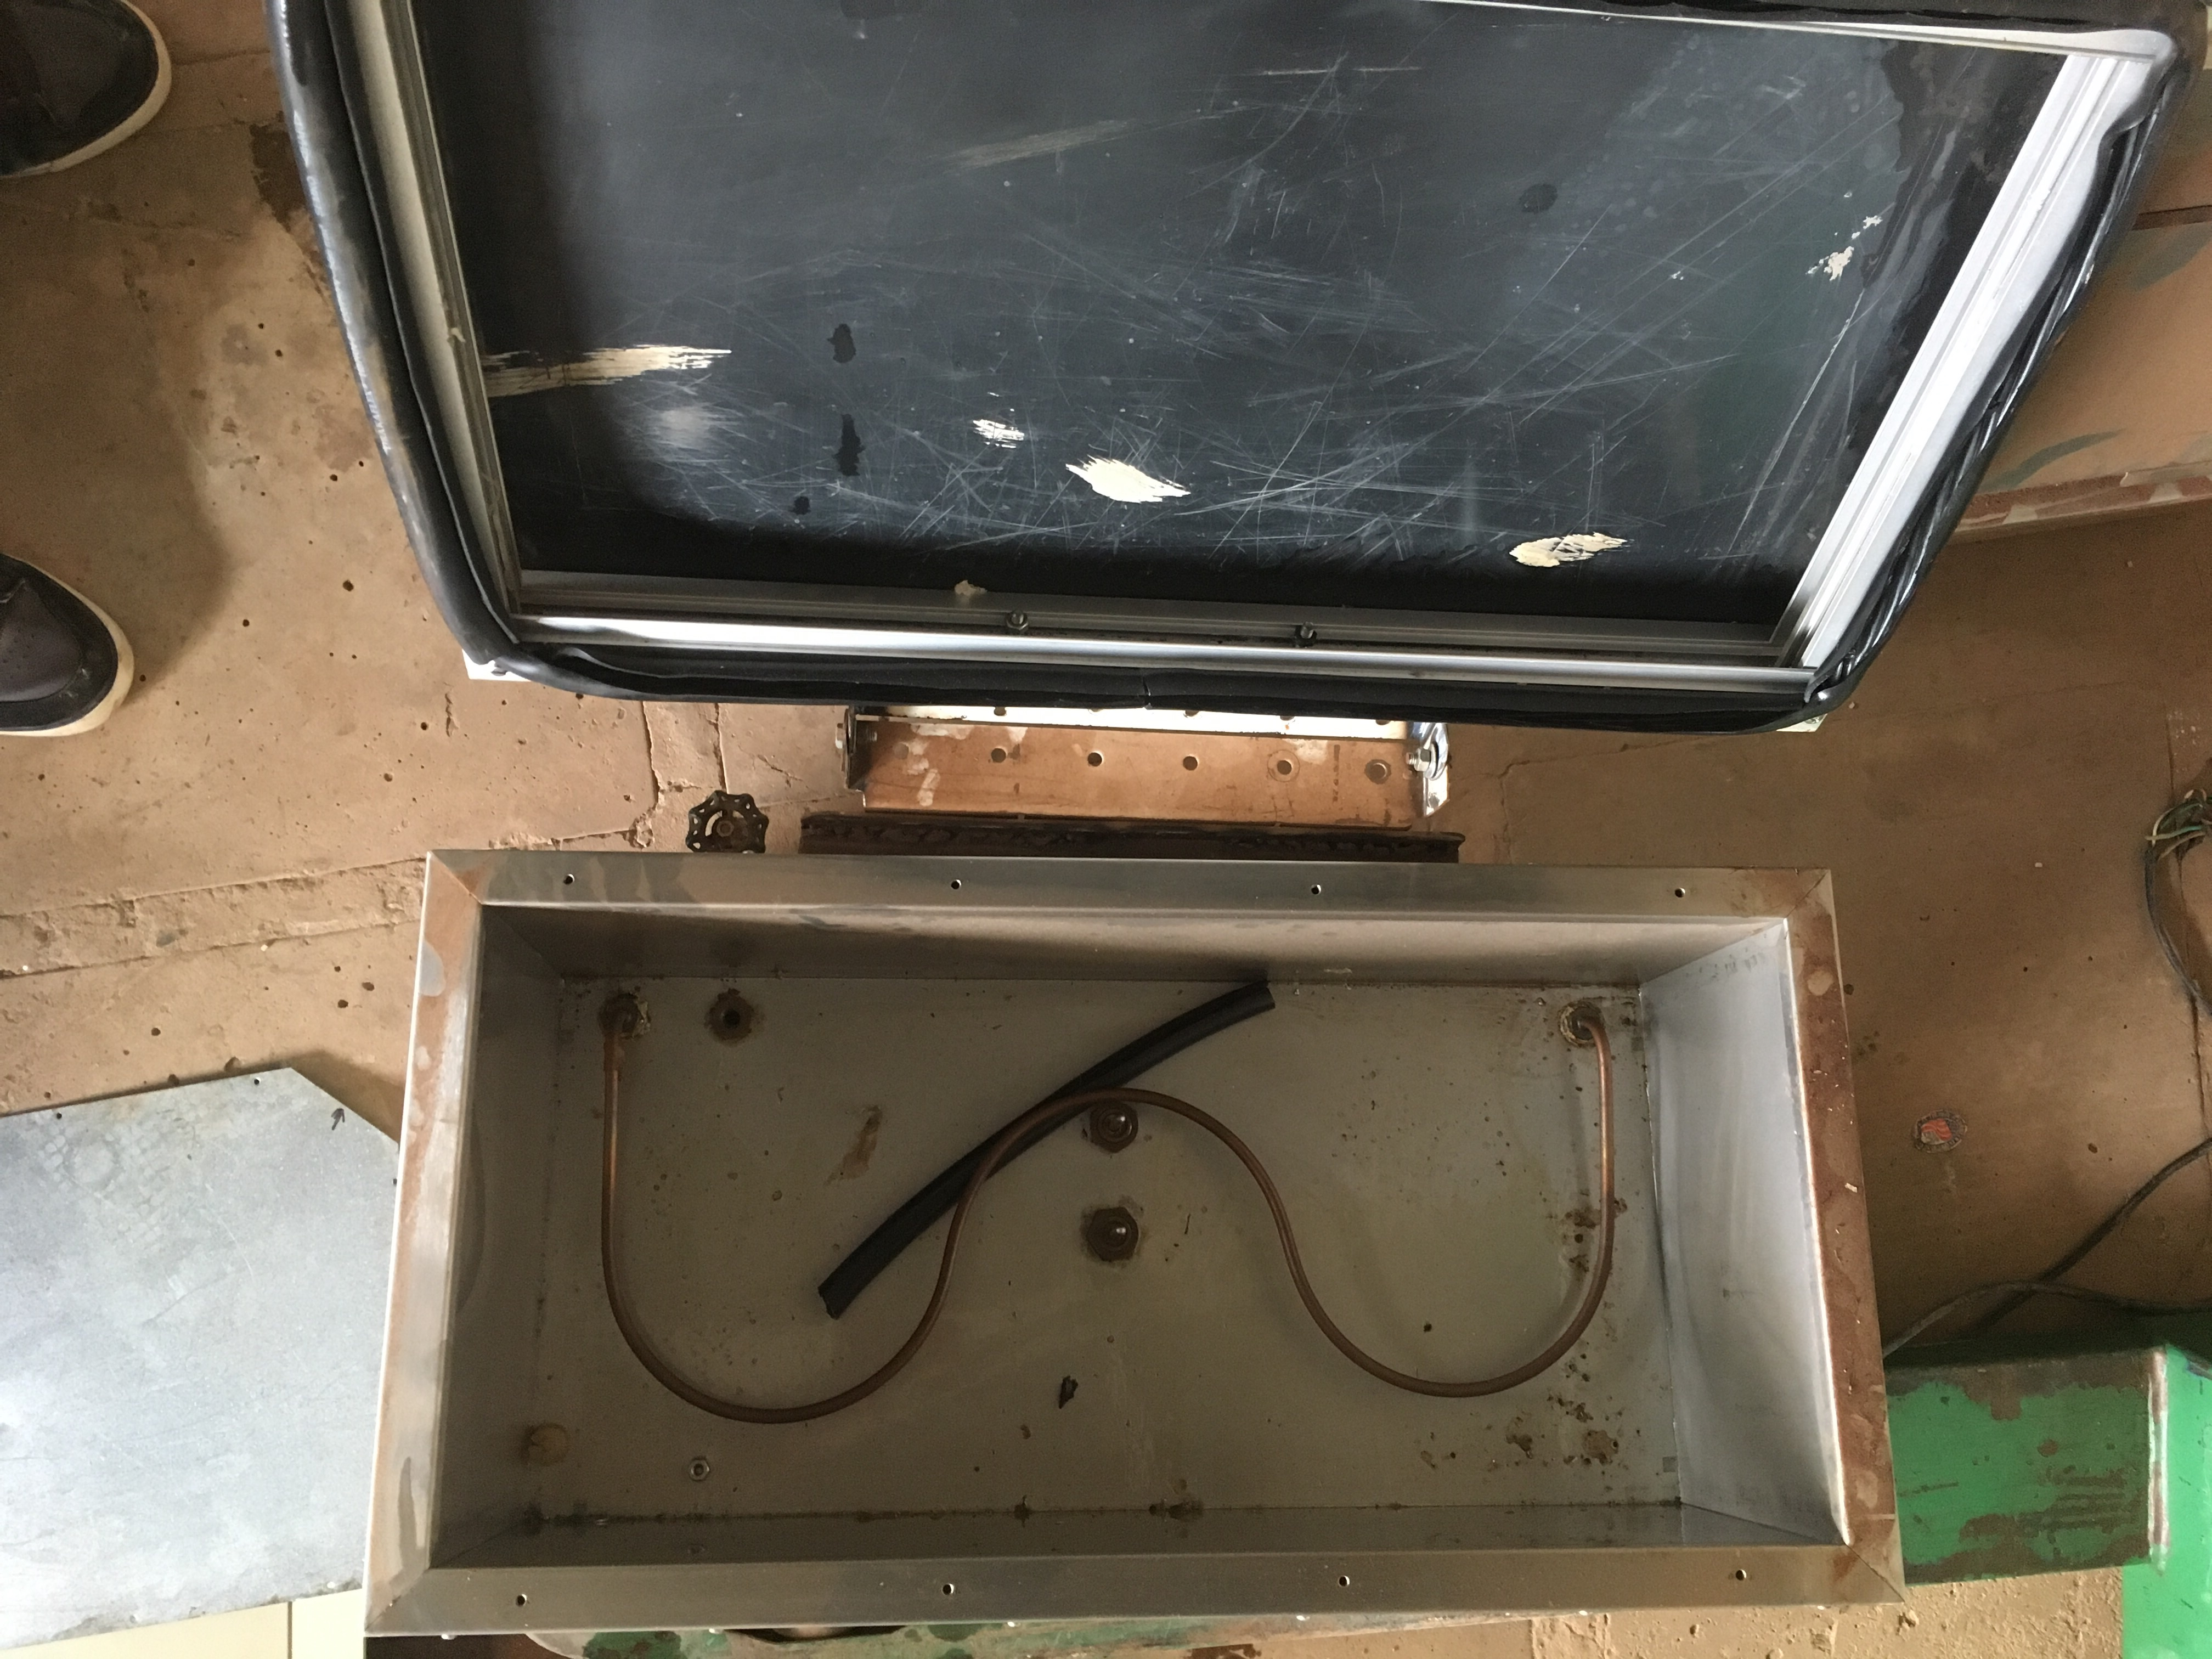
\includegraphics[width=0.4\textwidth]{figuras/freezer}
%     \caption{Estrutura base do freezer}
%     \label{fig:freezer}
% \end{figure}

A tampa que já estava presa ao freezer era instável e extremamente pesada, portanto optou-se por retirá-la e construir uma nova tampa para a estrutura. Além disso, os cortes necessários para o posicionamento da serpentina e para a queda dos picóles para outro compartimento foram feitos. O atual estado do freezer pode ser observado na figura \ref{fig:freezer_cortado}.

%    \begin{figure}[H]
% 	\centering
%    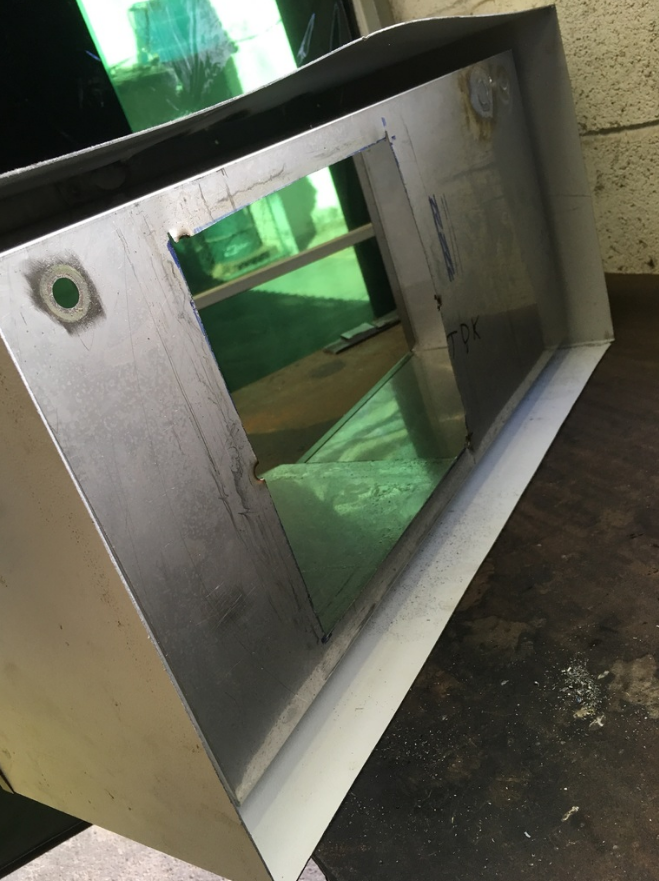
\includegraphics[width=0.4\textwidth]{figuras/freezer_cortado}
%     \caption{Estrutura do freezer depois do corte}
%     \label{fig:freezer_cortado}
% 	\end{figure}

\item Molas

A príncipio as molas seriam usinadas com diâmetro e passo especificados na figura \ref{fig:molas_dimensoes}). No entanto, a empresa de máquina de vendas Diletto Café emprestou molas (fig. \ref{fig:mola}) de aço inox  para o projeto, pois se tratando de uma máquina para alimentos a utilização de aço inoxidável é necessária afim de não contaminar o conteúdo perecível. A mola projetada apresentava espaço para 20 picolés, já a mola disponibilizada pela Diletto Café apresenta 19 espaços, possuindo perda de apenas 1 picolé por cada sabor. Logo, não apresenta grandes mudanças no estoque da máquina, além de ser uma solução mais econômica e com dimensões próximas as esperadas no projeto preliminar.

%    \begin{figure}[H]
% 	\centering
%    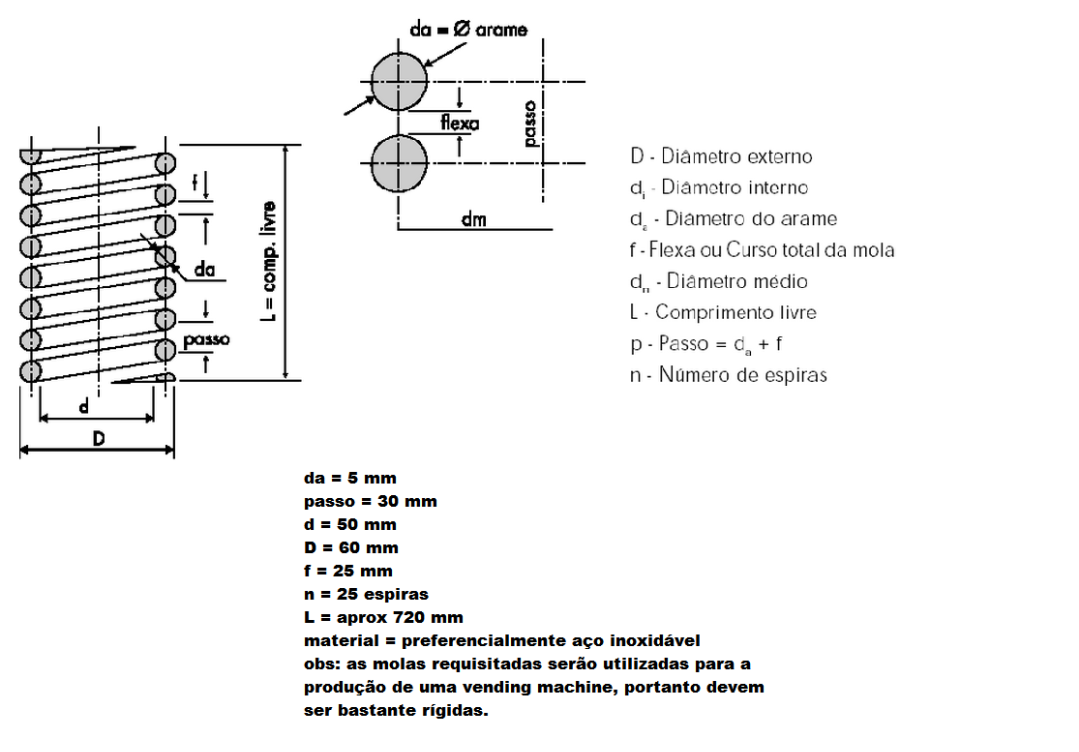
\includegraphics[width=\textwidth]{figuras/molas_dimensoes}
%     \caption{Desenho técnico das molas dimensionadas}
%     \label{fig:molas_dimensoes}
% 	\end{figure}

%    \begin{figure}[H]
% 	\centering
%    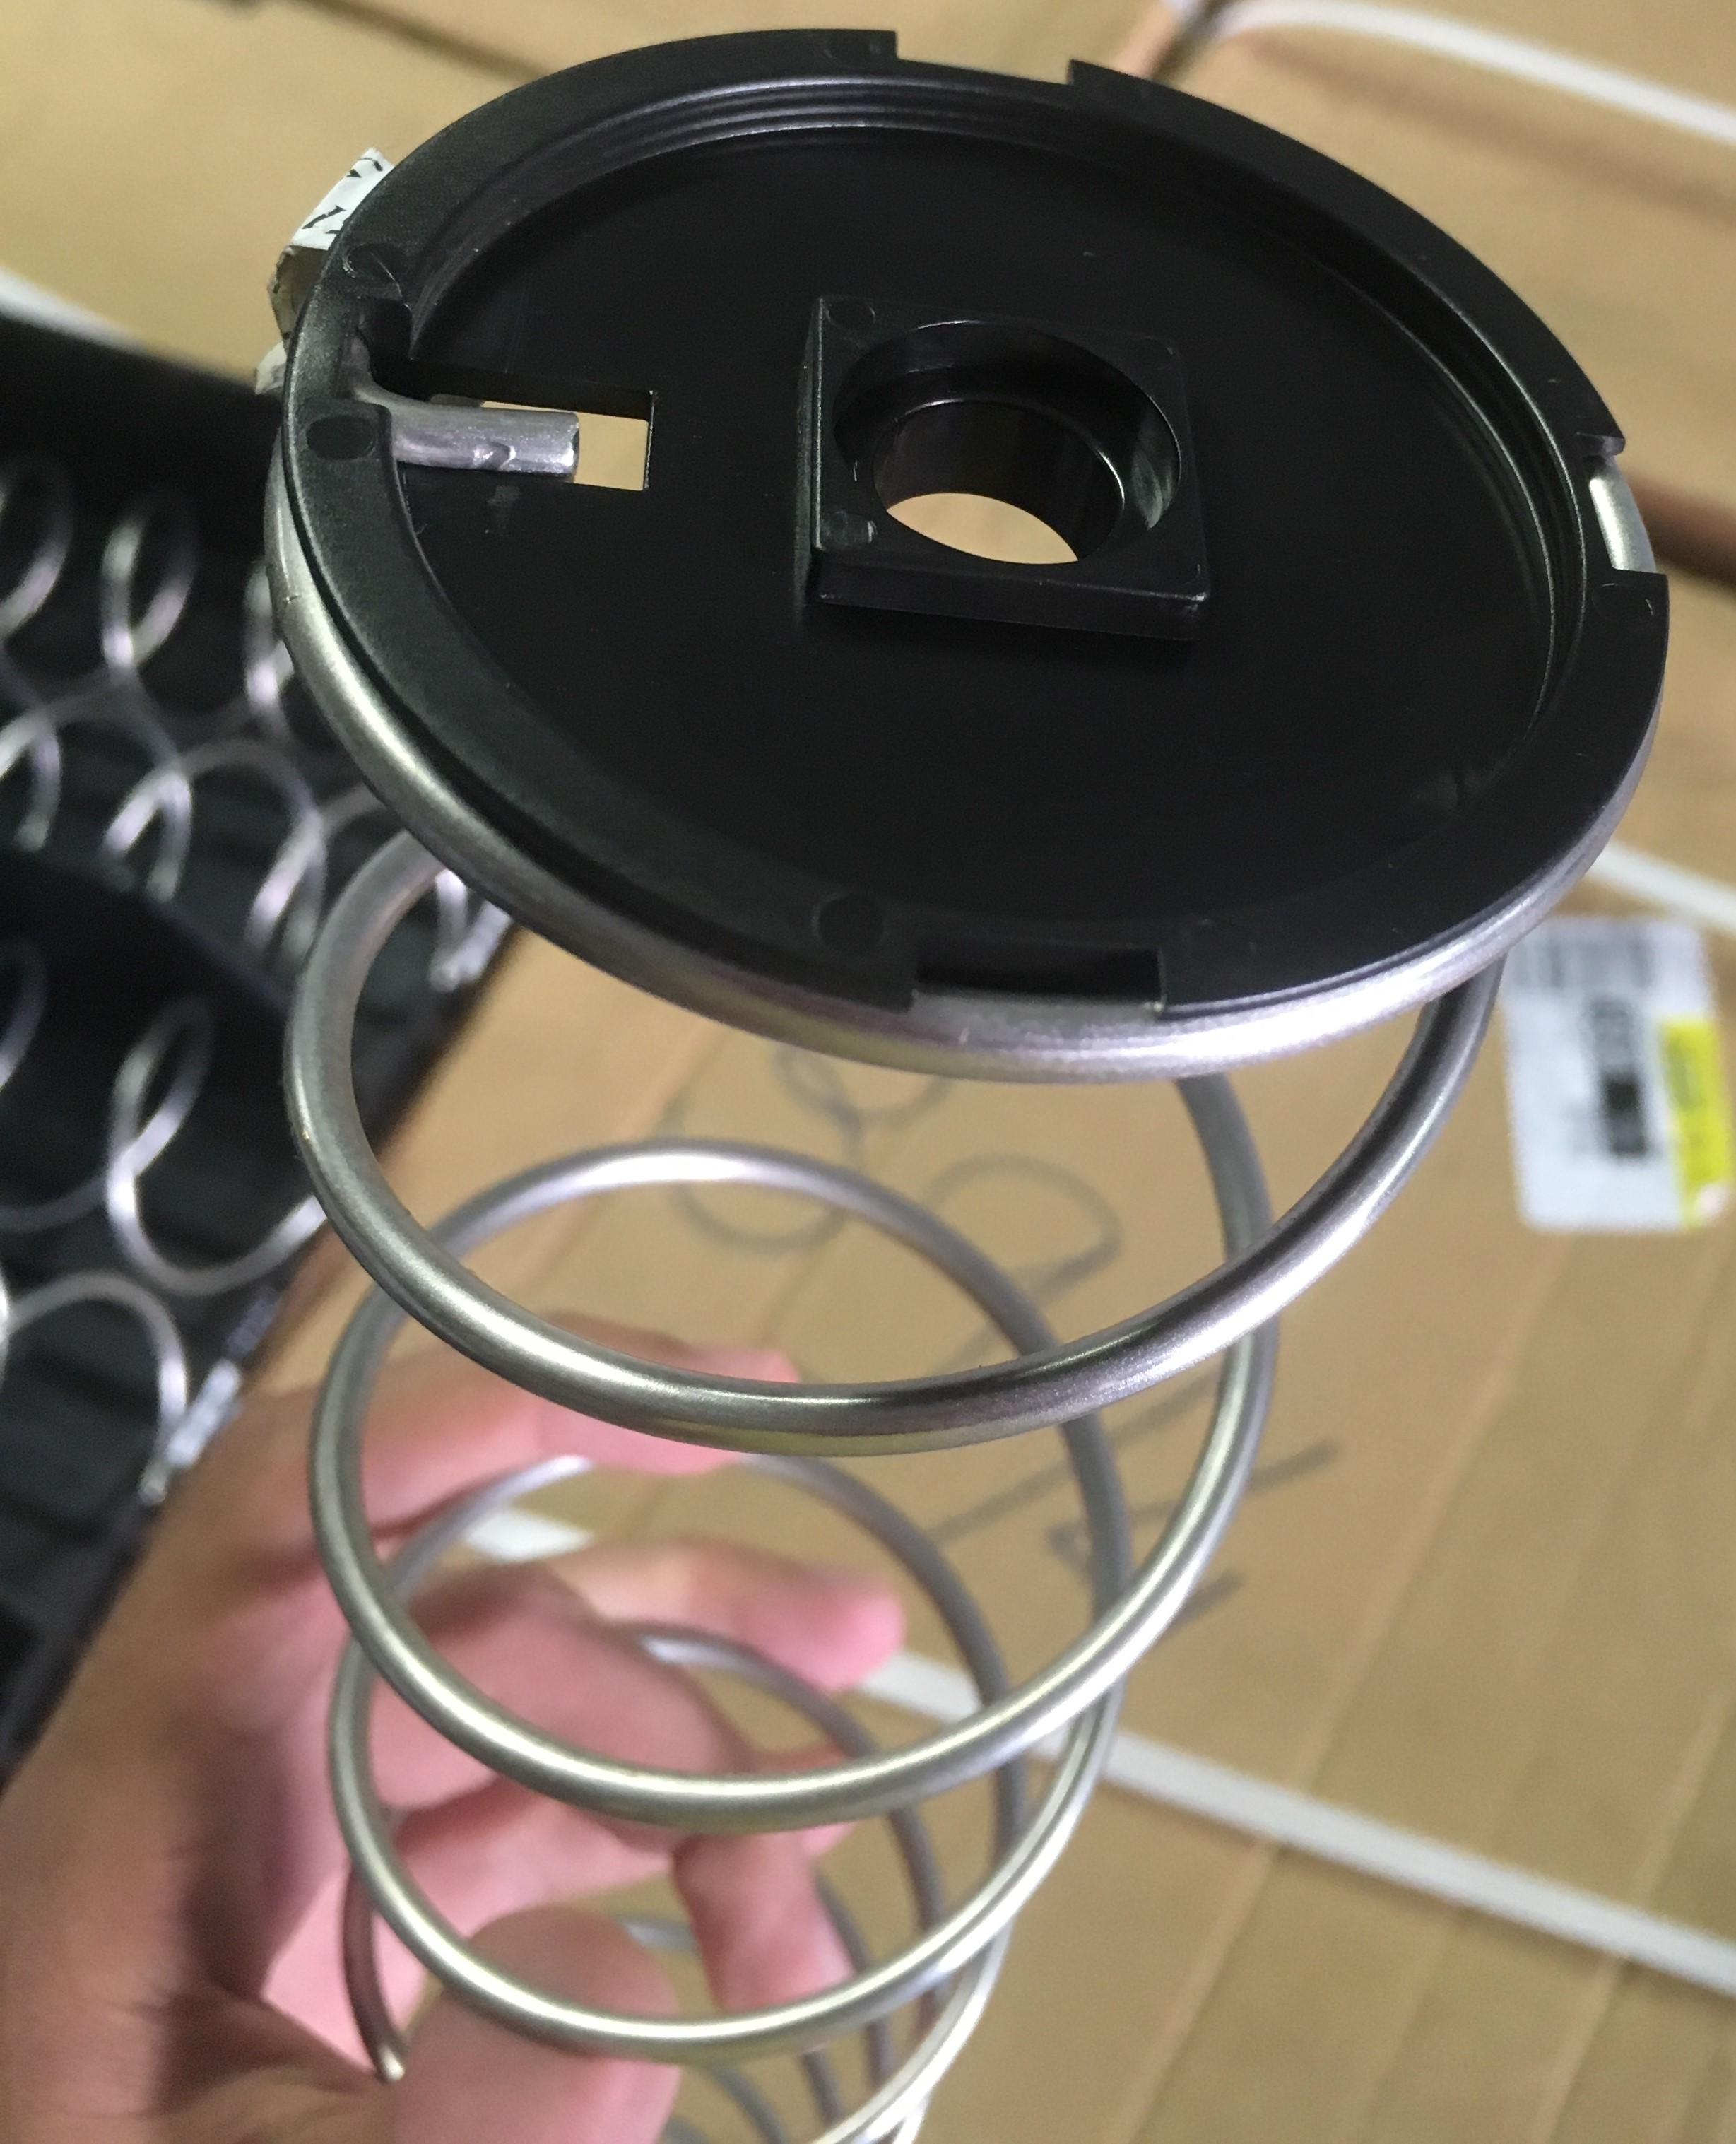
\includegraphics[width=0.4\textwidth]{figuras/mola}
%     \caption{Mola utilizada no projeto}
%     \label{fig:mola}
% 	\end{figure}

\item Caixa da serpentina do compressor

A serpentina do compressor (\ref{fig:serpentina}) precisa estar dentro da região refrigerada, pois ela é a responsável pelo resfriamento do freezer. Levando isso em consideração, uma caixa de aço foi soldada para servir como uma extensão do freezer, viabilizando o posicionamento da serpentina logo abaixo da grade onde deslizam os picolés. O desenho técnico da região resfriada encontra-se no anexo \ref{app:freezer}.

% \begin{figure}[H]
% \centering
% 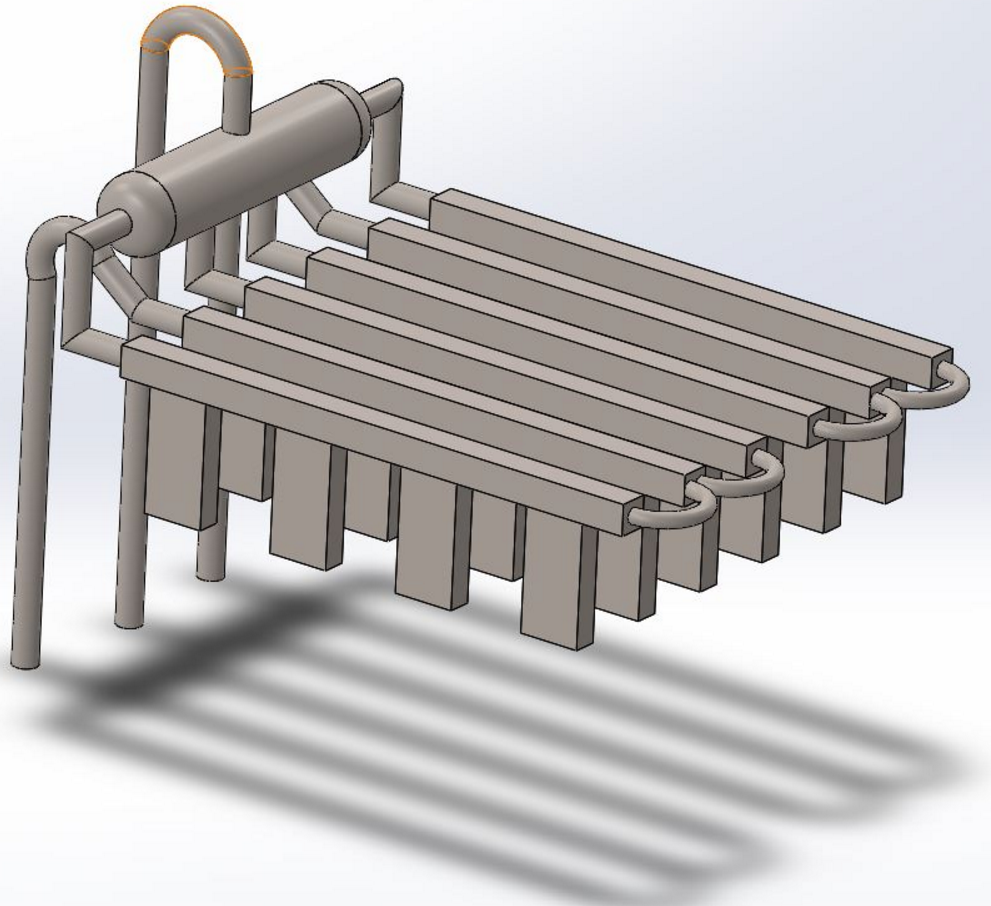
\includegraphics[width=0.4\textwidth]{figuras/serpentina}
%   \caption{CAD da serpentina}
% \label{fig:serpentina}
% \end{figure}

\item Carrinho para o transporte da máquina de vendas

	A massa total para a máquina está estimada em 87 quilogramas, logo para o transporte da mesma será necessário o uso de um suporte auxiliar. Esta será uma estrutura simples e que possa ser acoplada à máquina durante seu transporte e depois desacoplada para assim poder ser reutilizada no transporte de outra máquina de vendas. Existe uma  estrutura já pronta no galpão que é similar à figura \ref{fig:Render_-_Carro_de_Transporte}.

%    \begin{figure}[H]
% 	\centering
%     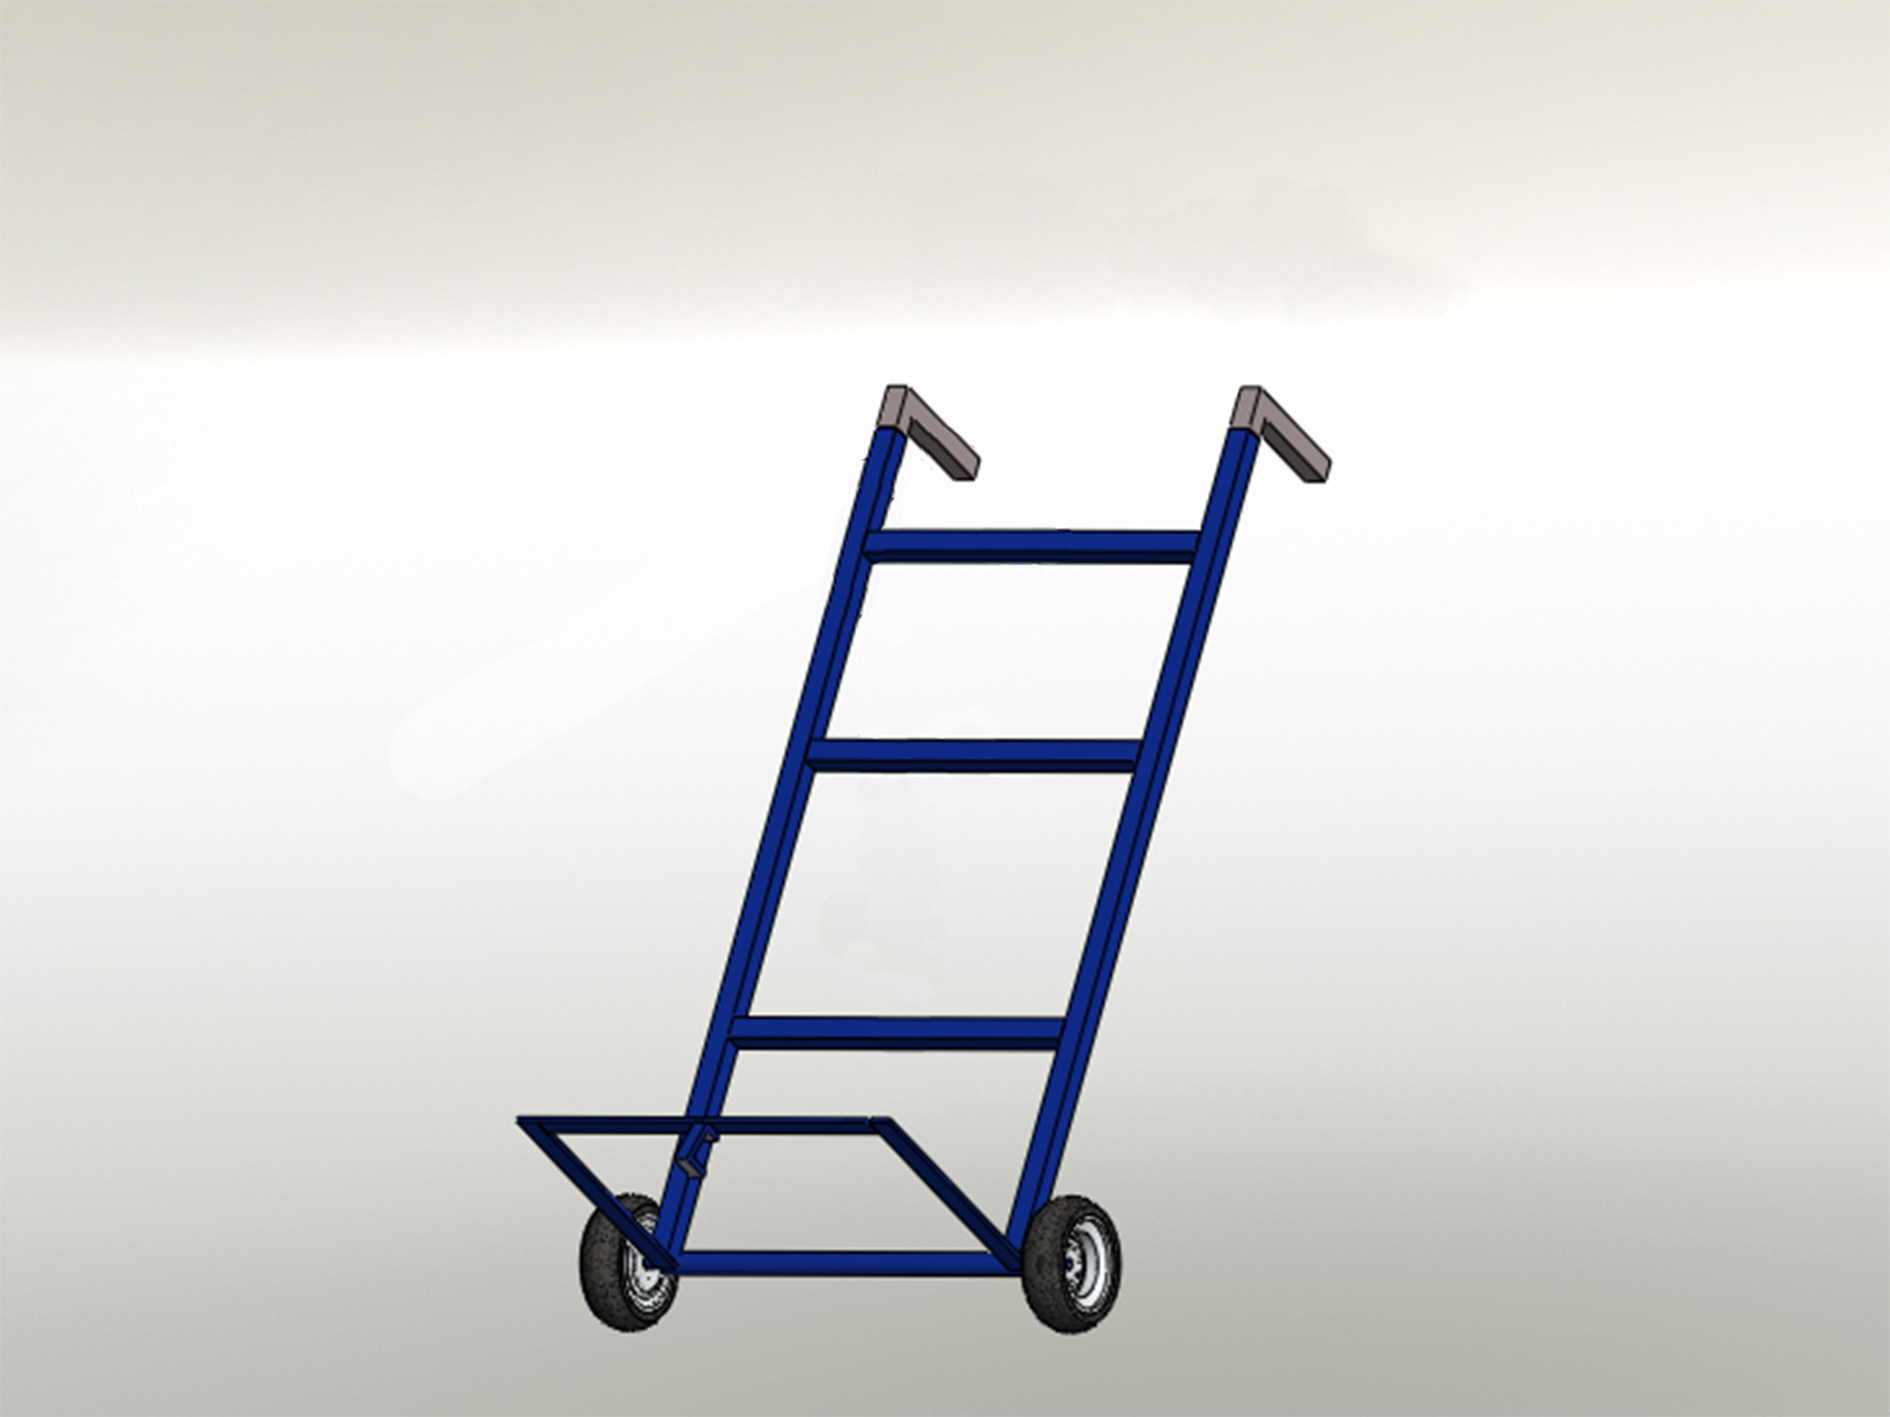
\includegraphics[width=0.4\textwidth]{figuras/Render_-_Carro_de_Transporte}
%     \caption{Estrutura base para o transporte da máquina de vendas}
%     \label{fig:Render_-_Carro_de_Transporte}
% \end{figure}

\subsection{Análise de temperatura em regime permanente e transiente (ANSYS)}

 Através dos softwares STEADY STATE e TRANSIENT THERMAL - MECHANICAL ANSYS MULTIPHYSICS, foi possível realizar uma análise da transferência de calor no freezer, com o objetivo de analisar o sistema de isolamento térmico além do sistema de resfriamento do freezer, que deve manter o picolé em uma temperatura apropriada. O método utilizado neste programa é o MEF (Método dos Elementos Finitos), onde o objeto de análise é discretizado em finitos elementos e utiliza-se um método numérico para solucionar as equações diferenciais parciais que determinam a temperatura e fluxo de calor variando no tempo em cada elemento, para um intervalo de tempo pré-determinado.
 Foram feitas algumas suposições e aproximações para possibilitar a análise da transferência de calor no sistema de refrigeração. Tais como:
\begin{itemize}
\item Representou-se a serpentina como uma caixa de volume aproximado;
\item Para a analise da transferência de calor através do ar interno do freezer, quando este tinha uma velocidade diferente de zero, aumentou-se seu coeficiente de condução já que não poderia ser propriamente representado como um fluido em movimento;
\item A serpentina foi representada por um sólido de temperatura constante durante a refrigeração do freezer, pois a serpentina é resfriada por fluido refrigerante R-22 mantido em circulação pelo compressor, o que geraria complicações na simulação;
\item Considerou-se a temperatura média da serpentina de -6,4\textdegree C, já que foi este o valor medido experimentalmente;
\item Suprimiu-se as molas, picolés e divisões internas do freezer para simplificar as simulações.
\end{itemize}
 As simulações feitas no regime estacionário tiveram as propriedades definidas como na tabela \ref{propestacionario}. Inicialmente pensou-se em isolar o freezer com isopor tanto externamente quanto internamente como na figura \ref{isolamento1}, além de utilizar PVC para forrar o freezer internamente. Porém observou-se, como mostrado na figura \ref{fig:isolamento_interno}, que a temperatura interna do freezer não baixava o suficiente. Logo optou-se por utilizar apenas isolamento externo como na figura \ref{isolamento2} e a nova simulação apresentou temperaturas bem mais baixas internamente, como mostrada na figura \ref{fig:sem_isolamento_interno}, confirmando que paredes de aço inox internamente era uma opção melhor. 
 
 \begin{table}[]
\centering
\caption{Propriedades para a simulação em regime estacionário e transiente}
\label{propestacionario}
\begin{tabular}{|l|l|}
\hline
\multicolumn{2}{|c|}{\textbf{Propriedades para a simulação em regime estacionário}}       \\ \hline
\textbf{Temperatura da Serpentina}   &  -6.4\textdegree C
\\ \hline
\textbf{Coeficiente de convecção exterior}    &    5W/$m^2$ \textdegree  C                 \\ \hline
\textbf{Temperatura média do ar exterior}     & 22\textdegree C                             \\ \hline
\end{tabular}
\end{table}

%     \begin{figure}[!htb]
%     	\begin{floatrow}
%         	\ffigbox{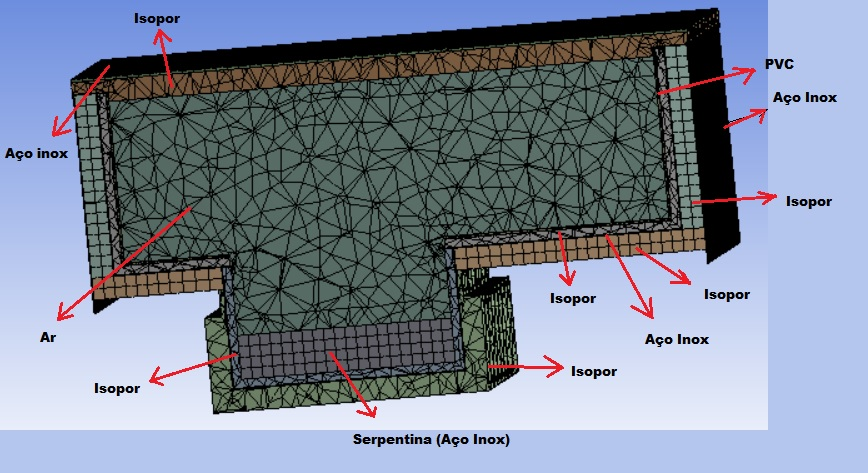
\includegraphics[scale=0.3]{figuras/isolamento1}}
%{\caption{Freezer com isolamento interno e externo}}
%     \label{fig:isolamento1}
%             \ffigbox{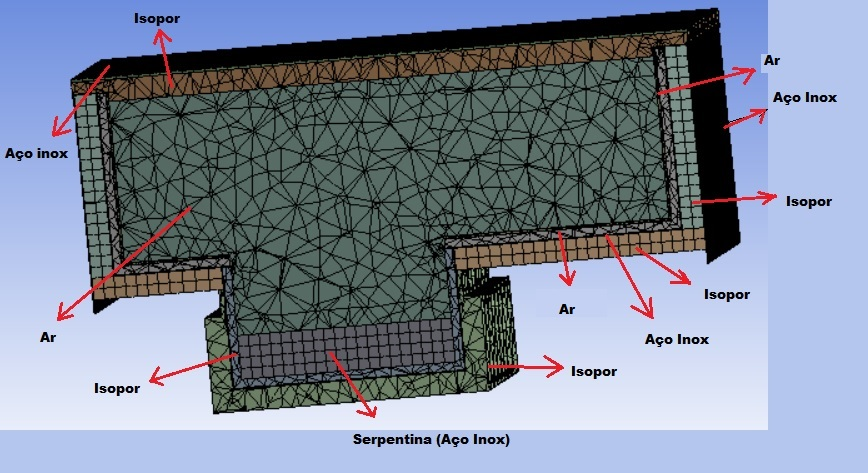
\includegraphics[scale=0.3]{figuras/isolamento2}}{\caption{Freezer sem isolamento interno}}
%     \label{fig:isolamento2}
%         \end{floatrow}
%     \end{figure}

%     \begin{figure}[!htb]
%     	\begin{floatrow}
%         	\ffigbox{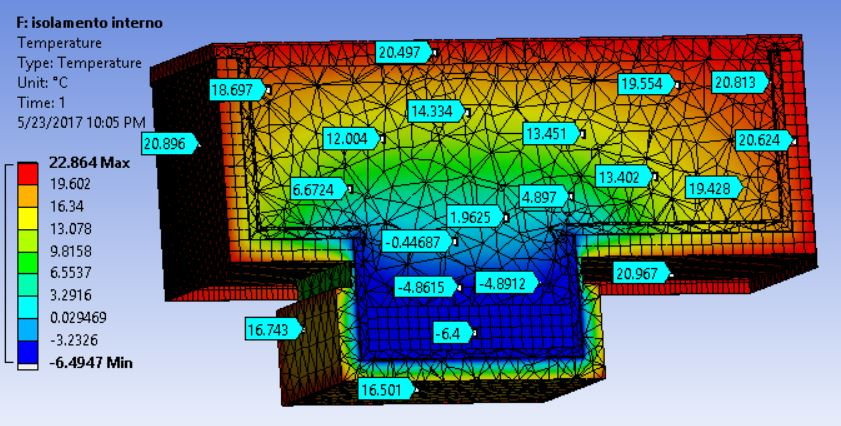
\includegraphics[scale=0.3]{figuras/isolamento_interno}}{\caption{Resultado da simulação do Freezer com isolamento interno}}
%     \label{fig:isolamento_interno}
%             \ffigbox{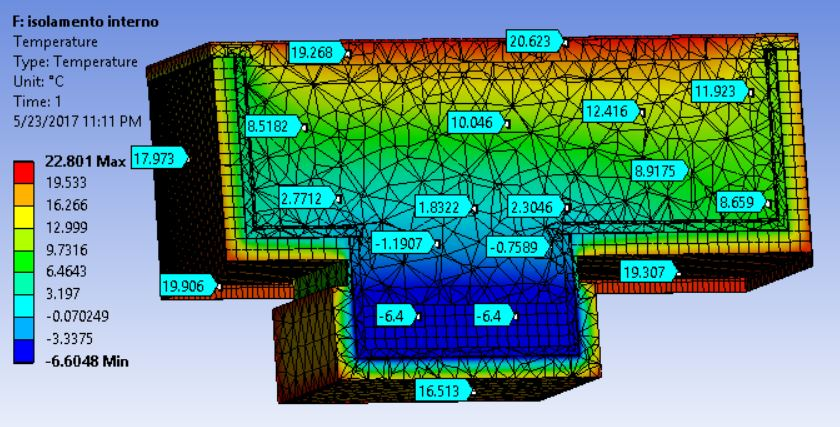
\includegraphics[scale=0.3]{figuras/sem_isolamento_interno}}{\caption{FResultado da simulação do Freezer sem isolamento interno}
%     \label{fig:sem_isolamento_interno}
%         \end{floatrow}
%     \end{figure}

\par O fato do freezer sem isolamento interno ser mais eficiente se deve ao fato do coeficiente de condução de calor do aço inox ser notavelmente mais alto do que o coeficiente de condução do isopor. Sendo assim, a presença de um isolamento interno no Freezer impede que as paredes do mesmo se mantenham resfriadas e, portanto, o ar interno é refrigerado apenas pela presença da serpentina. Quando não há isolamento interno, e o ar interno está diretamente em contato com as paredes de aço inox, que por sua vez estão em contato com a serpentina, o ar é refrigerado não apenas pela serpentina, mas também pelas paredes de aço que permanecem refrigeradas devido ao alto coeficiente de condução \cite{coeficiente}. 

\par Porém, observou-se que, mesmo com paredes de aço inox, a temperatura do freezer ainda não era a requerida para a conservação dos picolés. Para garantir a correta refrigeração dos picolés, foi decido instalar um cooler acima da serpentina para circular o ar interno do freezer e assim, garantir uma melhor refrigeração. Para simular a presença do cooler, foi necessário acrescentar uma condição de contorno de convecção internamente no freezer. Sendo assim, de acordo com a velocidade do ar interno, pode-se determinar o coeficiente de convecção interno, a partir da seguinte equação \cite{convection}, onde v é a velocidade relativo do ar em relação às paredes do Freezer:

$$
    h = 10,45 - v + 10 \sqrt[]{v}
$$

Observando-se que a equação acima só poderia ser aplicada para velocidades do ar entre 2m/s e 20m/s, optou-se por simular uma velocidade mínima de 2m/s, determinando assim um coeficiente de convecção interno de $22,6 W/m^2\textdegree C $. Além da convecção interna, foi preciso estabelecer um coeficiente de condução maior para o ar interno, já que este não está mais estagnado com a presença do cooler. Já que o simulador utilizado não suporta o cálculo das propriedades através de um fluido como o ar, foi preciso fazer uma aproximação onde o coeficiente de condução do ar interno deveria reproduzir o correto fluxo de calor através da convecção interna. Sendo assim, definiu-se um coeficiente de condução igual a $4 W/m\textdegree C$, calculado a partir das seguintes equações \cite{equacoesCOEF}: 

$$
    q_k = kA {\Delta T\over x}
$$
Onde $q_k$ é o calor transferido por condução através de uma parede plana, k é o coeficiente de condução, A é a área de troca de referência, $ \Delta T$ é a diferença de temperatura representativa entre a superfície quente e a superfície fria, e x é a espessura da parede.
$$
    q_h = hA \Delta T
$$
Onde $q_h$ é o calor transferido por convecção através de um fluido cujo coeficiente de convecção é h. 
Para que $q_k$ seja igual à $q_h$, então:
$$
    k = hx
$$
Logo considerou-se a região com o menor coeficiente de condução possível, onde x era menor, chegando-se à $4 W/m\textdegree C$. Assim sendo, temos o resultado da simulação para o caso aproximado onde haveria a presença de um cooler dentro do freezer, cujo resultado é mostrado na figura \ref{fig:simulacao_cooler}.

%    \begin{figure}[H]
% 	\centering
%     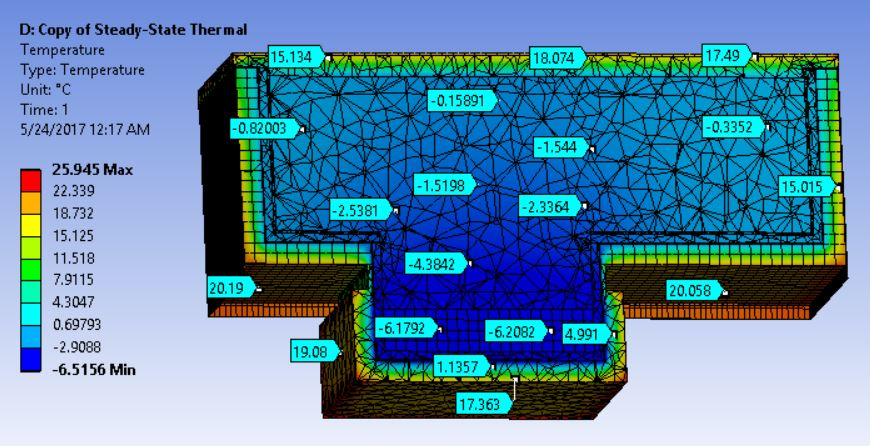
\includegraphics[width=0.4\textwidth]{figuras/simulacao_cooler}
%     \caption{Resultado da simulação em regime estacionário com convecção interna e externa}
%     \label{fig:simulacao_cooler}
% \end{figure}

Após concluir as simulações em regime estacionário, foi possível realizar uma simulação em regime transiente, utilizando-se como base as propriedades e condições de contorno utilizadas na simulação com convecção interna e externa, onde analisou-se 10000s de funcionamento do Freezer, onde em 5400s observou-se que o Freezer já atingia temperaturas abaixo de zero em sua maior parte. Como resultado, temos que o Freezer estaria com o ambiente apropriado para o armazenamento dos picolés após aproximadamente uma hora e meia refrigerando, como visto na Figura \ref{fig:temp_5402}.

%     \begin{figure}[!htb]
%     	\begin{floatrow}
%         	\ffigbox{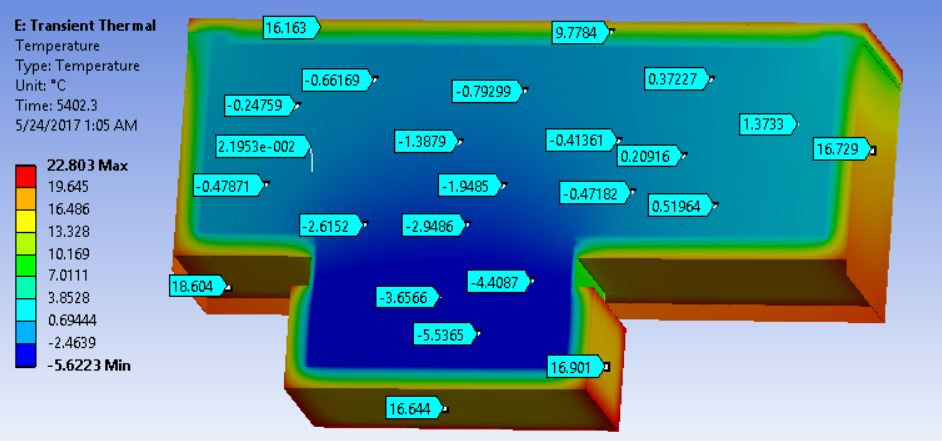
\includegraphics[scale=0.5]{figuras/temp_5402}}
%{\caption{Resultado da simulação para regime transiente após aproximadamente uma hora e meia desde a ativação do compressor}}
%     \label{fig:temp_5402}
%             \ffigbox{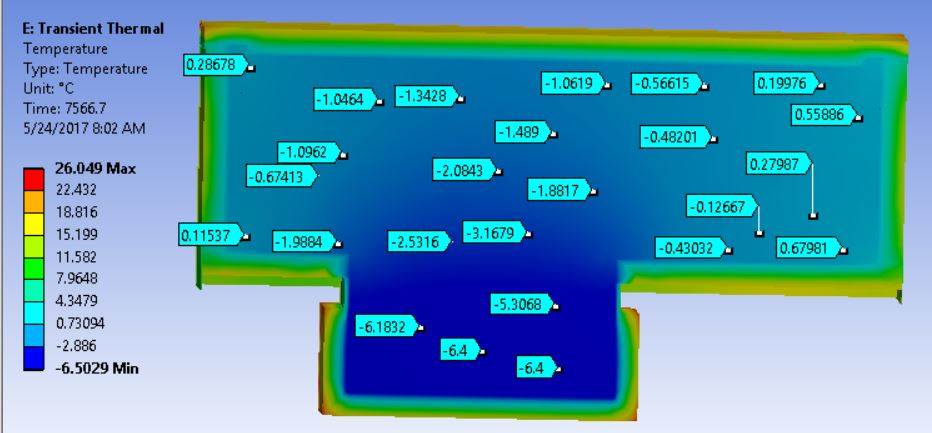
\includegraphics[scale=0.5]{figuras/temp_7566}{\caption{FResultado da simulação para regime transiente após pouco mais de duas horas desde a ativação do compressor}
%     \label{fig:temp_7566}
%         \end{floatrow}
%     \end{figure}

Observando-se os gráficos mostrados nas Figuras \ref{fig:graph1} e \ref{fig:graph2}, tem-se que a temperatura do Freezer se estabiliza em torno dos 7566s - aproximadamente 36min após atingir o ambiente necessário para os picolés, como mostrado na Figura \ref{fig:temp_7566}. Logo, este seria o momento ideal para se desligar o compressor e ao fazer isso, o Freezer manteria um ambiente apropriado para os picolés por aproximadamente 15min, como mostrado na figura \ref{fig:temp_8566}, após esse período o compressor deveria ser religado e permanecer por aproximadamente 30min - tempo aproximado para a temperatura interna se estabilizar - para ser em seguida desligado novamente por 15min, seguindo assim um ciclo onde em 67\% do tempo o compressor estaria ligado.. Estes resultados da simulação serão validados experimentalmente e, caso provem-se distantes da realidade, serão adaptados para melhor representar o caso real. 

%    \begin{figure}[H]
% 	\centering
%     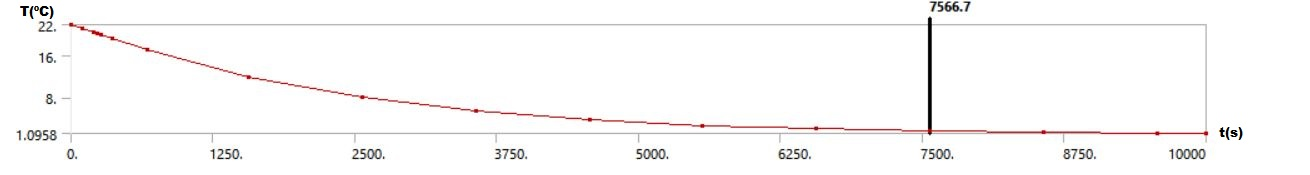
\includegraphics[width=0.8\textwidth]{figuras/graph1}
%     \caption{Gráfico da temperatura média nas paredes do freezer em função do tempo}
%     \label{fig:graph1}
% \end{figure}

%    \begin{figure}[H]
% 	\centering
%     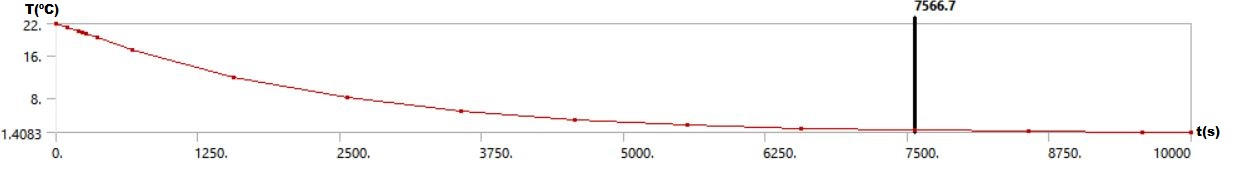
\includegraphics[width=0.8\textwidth]{figuras/graph2}
%     \caption{Gráfico da temperatura média na face inferior do interior do freezer em função do tempo}
%     \label{fig:graph2}
% \end{figure}

%    \begin{figure}[H]
% 	\centering
%     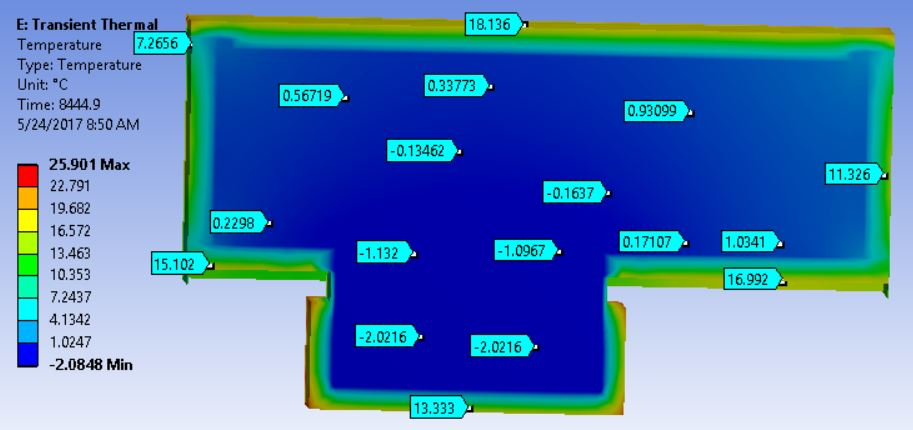
\includegraphics[width=0.6\textwidth]{figuras/temp_8444}
%     \caption{Resultado da simulação para regime transiente após aproximadamente quinze minutos desde a desativação do compressor}
%     \label{fig:temp_8444}
% \end{figure}

\end{itemize}


\section{Solução de Energia}

Os subsistemas de energia estão divididos conforme a organização desta secção.

\subsection{Refrigeração}
Atendendo aos requisitos definidos para o projeto, o recipiente no qual os picolés são armazenados  mantém-se refrigerado durante o período de venda. O processo de refrigeração consiste em retirar calor de uma corpo ou espaço para reduzir sua temperatura e transferir esse calor para outro corpo ou espaço \cite{campos2010refrigeraccao}. Portanto, a partir da análise das características da demanda de refrigeração, custos limitados e o tempo hábil para a construção e integração do produto em questão, encontrou-se duas opções de resfriamento:

\begin{itemize}
\item Células de Peltier;
\end{itemize}

\begin{itemize}
\item Compressor;
\end{itemize}

O módulo de Peltier é a maneira mais prática de se utilizar o efeito peltier em larga escala, e consiste em um arranjo de pequenos blocos de \textit{telureto de bismuto - $Bi_{2}Te_{3}$} dopados tipo N e tipo P montados alternamente e eletricamente em série entre duas placas de cerâmica com alta condutividade térmica.Os semicondutores utilizados possuem altos coeficientes de Seebeck e podem ser tipo N $(\alpha \leq 0)$ e tipo P $(\alpha \geq 0)$  \cite{campos2010refrigeraccao}.

A utilização dos módulos de peltier tem as seguintes vantagens:

-Não utiliza partes mecânicas móveis para refrigeração;

-Aquece e resfria dependendo apenas da polaridade da alimentação;

-Dispensa o uso de gases refrigerantes, tecnologia 100 por cento estado sólido;

-Funcionam em qualquer orientação com/sem gravidade diferente dos refrigeradores baseados em compressores.


O resfriamento utilizando compressores ocorre por meio da compressão mecânica de vapor de um fluido refrigerante. Fluido refrigerante é uma substância que, ao circular dentro de um circuito fechado, é capaz de retirar calor de um meio enquanto se vaporiza a baixa pressão \cite{teixeiraconcepccao}.

Ao se optar pelo resfriamento por compressão tem-se as seguintes vantagens:

\begin{itemize}
\item Baixo consumo;

\item Maior Eficiência;
\end{itemize}


Outra opção a ser utilizada no projeto é o resfriamento por meio de compressor, uma vez que o consumo da célula de peltier é extremamente alto, 70W para a placa de 40x40x4 milímetros. Para resfriar o recipiente seriam necessários entre 7 a 10 módulos, o que necessitaria uma fonte de 490W a 700W e um inversor. A fonte de fornecimento escolhida foi placas fotovoltaicas e para conseguir manter esse fornecimento seria necessário uma área para absorção de energia solar muito maior do que seria possível instalar na máquina de vendas de picolé.


Para o dimensionamento do compressor, é necessário calcular a potência necessária para fazer o fluido refrigerante circular pela serpentina. Essa potência foi encontrada a
partir da formulação:

\begin{math} W_{c} = m_{f} * (h_{2} - h_{1})  \end{math}

Onde:

$W_{c}$ é a potência teórica do compressor (kJ/h);

$m_{f}$ é o fluxo de massa refrigerante (kg/h);

$h_{2}$ é a entalpia no inicio da compressão (kJ/kg);

$h_{1}$ é a entalpia no final da compressão (kJ/kg);


\subsection{Alimentação}
	As fontes de energia que serão utilizadas para alimentar o sistema de refrigeração da máquina de picolé são painéis fotovoltaicos e baterias. O painel solar será dimensionado levando em conta a demanda energética a qual a mesma supre para manter o banco de baterias em condições de manter o refrigerador em operação durante o período solicitado, bem como os outros equipamentos consumidores e referentes às outras áreas.

  \begin{itemize}
    \item Diagrama Elétrico Simplificado
    	Abaixo, temos um diagrama elétrico simplificado da \textit{Vending Machine}, ele representa o circuito de alimentação utilizado, desde a geração de energia até o uso final. Este diagrama será refinado e detalhado no último ponto de controle, pois o sistema poderá sofrer algumas modificações e adições, tais como sistema de proteção e sistema externo auxiliar para o compressor.

%        \begin{figure}[H]
%     \centering
%     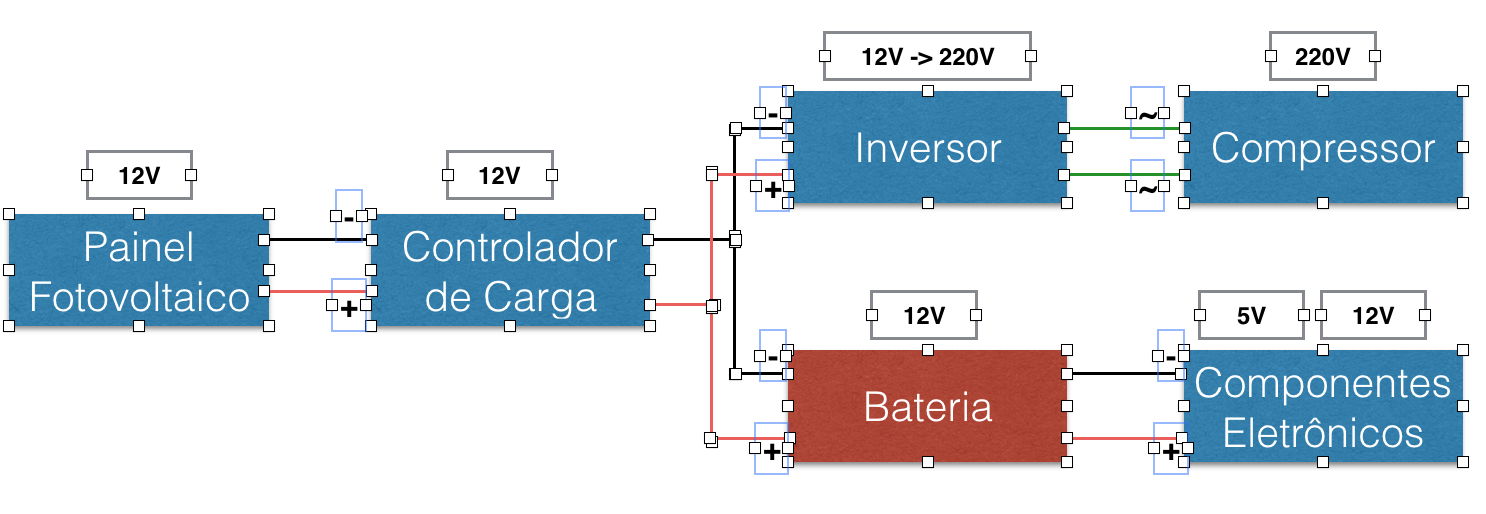
\includegraphics[width=0.7\textwidth]{figuras/diagrama_simplificado}
%     \caption{Diagrama Elétrico Simplificado}
%     \label{fig:diagrama_simplificado}
% \end{figure}

		A seguir detalharemos cada um dos elementos do sistema, bem como o seu dimensionamento e características principais.

\end{itemize}


\begin{itemize}
\item Painel Fotovoltaico
\end{itemize}
		A tomada de decisão para escolha de um painel fotovoltaico deve considerar a demanda energética dos sistemas os quais serão alimentados, no caso da máquina de vendas especificamente, deverá carregar a bateria que alimentará o compressor, e deixa-la em condições de uso durante o período solicitado. A tensão gerada pela placa deverá ser elevada para atender às necessidades do compressor, para isso um inversor será instalado, bem como um controlador de carga.
        Para o dimensionamento prático e inicial do gerador fotovoltaico é válida a seguinte expressão:

\begin{eqnarray}
Potência mínima do gerador (Wp) = \frac{\text{Consumo Total}(Wh/dia) }{\text{Horas equivalentes de sol pleno} (h/dia) x Fpp x Fps}
\end{eqnarray}

        A quantidades de horas equivalentes de Sol pleno (horas/dia) depende da latitude e nível de nebulosidade do local considerando o nível médio do mês mais crítico no plano escolhido para instalar o módulo. A inclinação do módulo será zero. No Brasil considera-se entre 3,5 e 5 horas/dia de Sol pleno para o pior mês. Para Brasília foi adotado o valor de 4 horas.

        O fator de perda de potência (FPP) pode ser estimado dividindo-se a tensão da bateria pela tensão de máxima potência do módulo a ser utilizado. Esta perda se deve ao fato da tensão da bateria (12 V) ser inferior à tensão de máxima potência do módulo a ser utilizado (Vmp=+/-16,6 V para os módulos Yingli). Um valor prático 12 V/16,6 V = 0,72. Estas perdas podem ser reduzidas através do uso de um controlador de carga com seguidor de máxima potência (MPPT).
        Saber o fator de perdas e segurança (FPS) é necessário para levar em conta a redução da geração do módulo devido à tolerância na fabricação (os módulos normalmente tem uma tolerância em relação à potência nominal de +/-3\%), temperatura de trabalho (quase sempre maior que os 25ºC da condição padrão de testes), poeira sobre o vidro, degradação com o tempo, presença de sombras em parte do dia, desvios na orientação e na inclinação e também devido às perdas elétricas na bateria, no controlador e na fiação, além de incertezas sobre os dados utilizados e o consumo previsto. Valor típico adotado é de 0,8.

\begin{eqnarray}
Potência mínima do gerador (Wp) = \frac{\text{1880}(Wh/dia) }{\text{4} (h/dia) x 0,72 x 0,8} = 815 Wp
\end{eqnarray}

        A decisão de escolha do painel teve como variáveis a disponibilidade e custos de implementação foram limitantes, uma vez que um painel com essa potencia custa aproximadamente 7 mil reais. Dessa forma essas variáveis corroboraram para que um painel de 20Wp, disponibilizado por um integrante do grupo, fosse escolhido e funcionará de maneira análoga a um painel de grande porte, e ainda que de baixa potência,  auxiliará no processo de recarga da bateria.
        O painel da marca \textit{Yingli Solar - Power Your Life},  será utilizado e possui as seguintes especificações:

\begin{table}[]
\centering
\caption{My caption}
\label{my-label}
\begin{tabular}{|l|l}
\cline{1-1}
\textbf{Yingli Solar-YL020P-17B 1/7} &                                    \\ \hline
\textbf{Potência {[}W{]}}                                                           & \multicolumn{1}{l|}{\textbf{20}}   \\ \hline
\textbf{Tensão {[}V{]}}                                                             & \multicolumn{1}{l|}{\textbf{16,6}} \\ \hline
\textbf{Corrente {[}A{]}}                                                           & \multicolumn{1}{l|}{\textbf{1,2}}  \\ \hline
\textbf{Tensão Circuito Aberto {[}V{]}}                                             & \multicolumn{1}{l|}{\textbf{21,4}} \\ \hline
\textbf{Tensão Máxima do Sistema {[}V{]}}                                           & \multicolumn{1}{l|}{\textbf{50}}   \\ \hline
\end{tabular}
\end{table}

        	De acordo com o selo PROCEL em parceria com o INMETRO, esse painel possui uma eficiência do tipo D, correspondente à 11,8\%, o que é compatível com outros painéis comerciais.
            A área externa do módulo \textit{Yingli Solar-YL020P-17B 1/7} é de $0,17m^{2}$, possui uma produção média mensal de energia de 2,50kWh/mês, esse valores são importantes para que seja observado que um painel de maior dimensão apresentaria um melhor comportamento quando associado na \textit{Vending Machine}, mas por viabilidade econômica não será possível a implementação de um painel maior.
            Abaixo, uma foto do painel que sera instalado.

%  \begin{figure}[H]
%     \centering
%     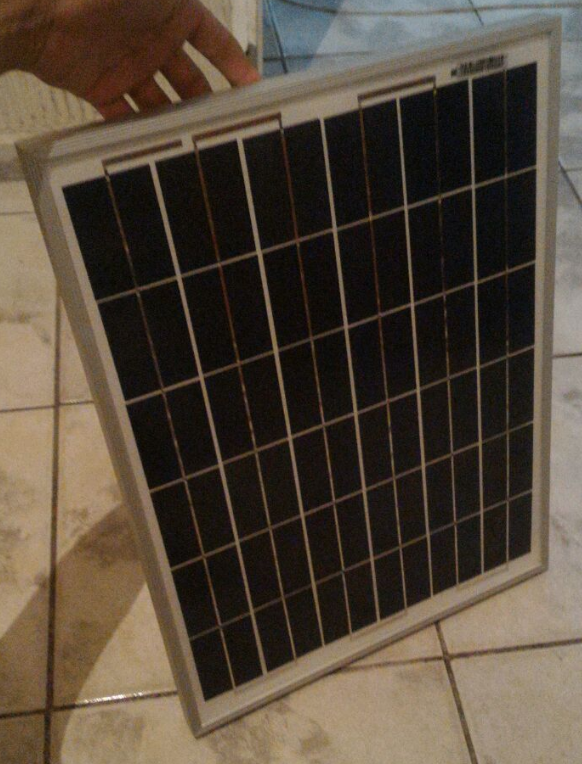
\includegraphics[width=0.7\textwidth]{figuras/painel_solar01}
%     \caption{Yingli Solar-YL020P-17B 1/7 }
%     \label{fig:painel_solar01}
% \end{figure}

\begin{itemize}
\item Bateria
\end{itemize}

      A tomada de decisão para escolha de uma bateria deve considerar a tensão e a corrente.  \cite{de2011}. O cálculo de autonomia de uma bateria necessita de diversos dados. Existem 3 parâmetros os quais são considerados os principais para a a escolha de uma bateria: curva de descarga, capacidade de armazenamento e capacidade de descarga \cite{meggiolaro2006tutorial}. A curva de descarga é a relação do decaimento da tensão ao longo do consumo da capacidade nominal. A capacidade da bateria quantifica o tempo para que ocorra uma descarga total, medido em Ah (Ampér hora). A capacidade de descarga é a quantificação da entrega de carga sem que ocorram danos à bateria.
      As baterias de chumbo-ácido são muito utilizadas em sistemas onde a há correntes  elevadas, como motores de arranque e máquinas elétricas. É composta por Chumbo e Ácido Sulfúrico em concentrações calculadas que variam de 27 à 37 por cento \cite{de2005estudo}, podendo ser seladas ou não, possuindo vida útil de até 4 anos, apresentando assim uma boa relação de custo-benefício.

\begin{itemize}
\item Decisão da Bateria - Veicular x Estacionária
\end{itemize}

		Uma das decisões voltadas ao fornecimento de energia do projeto foi quanto ao do tipo de bateria que iria auxiliar no funcionamento da \textit{Vending Machine}. Para isso, foram analisados os tipos de bateria existentes no mercado, como as baterias automotivas, como o próprio nome já diz, são desenvolvidas para o uso em automóveis, com uma vida útil estimada de aproximadamente 3 anos, e com capacidade de suportar correntes de pico elevadas por um curto período de tempo, e as baterias de característica estacionária, as quais são construídas com materiais mais nobres, visando aumentar a sua vida útil e eficiência, relacionado diretamente à sua finalidade de manter equipamentos em funcionamento pleno.
    	Uma análise feita nas especificações técnicas e características de ambas as baterias, como suas respectivas curvas de descarga, quantidade de ciclos em situação de uso diário, bem como a capacidade de suportar uma corrente elevada por um período de tempo maior, quando comparada às automotivas, tornam a bateria estacionária para o uso de equipamentos\textit{ off-grid}, a mais indicada.
   		A \textit{Vending Machine}, por ser um dispositivo que armazena produtos perecíveis, possuir uma câmara fria, além de ser um produto que tem como pré-requisito uma baixa manutenção, onde a confiabilidade do equipamento é um ponto muito importante, a bateria estacionária é a mais indicada para atender à proposta do equipamento, pela sua segurança, confiabilidade e comportamento mais estável além de suportar melhor descargas mais profundas, quando comparado com a uma bateria automotiva.

\begin{itemize}
\item Dimensionamento da Bateria
\end{itemize}

Para dimensionar a bateria foi necessário definir o consumo médio diário de energia elétrica, ou seja, definir a curva de carga, tanto em termos diários quanto sazonais. Com esses dados foi possível visualizar as características previstas para o consumo de eletricidade, adequando-se o sistema para que o consumo e a produção fossem compatíveis ao longo do dia e ao longo do ano.
		A \textit{Vending Machine} possui dispositivos consumidores de energia elétrica, e para o dimensionamento de um sistema eficiente e confiável, é preciso analisar a relação de consumo energético, tempo de funcionamento do equipamento e energia disponível na bateria. Para isso, foi feito um levantamento da potência consumida pelos principais equipamentos e relacionados com o tempo de operação da máquina.

\begin{table}[]
\centering
\caption{Relação de Consumo}
\label{my-label}
\begin{tabular}{|l|l|l|l|l|}
\hline
           & Potência {[}W{]} & Corrente {[}A{]} & Tensão{[}V{]}  \\ \hline
Compressor & 337            & 1,53           & 220           \\ \hline
Eletrônica & 38,2                & 3,18                 &12         \\ \hline
Iluminação & 5            & 0,41            & 12          \\ \hline
\end{tabular}
\end{table}

        Com uma relação dos principais consumidores de energia da \textit{Vending Machine} é possível ter uma média de consumo, e com isso relacionar ao tempo em que a bateria alimentará o sistema de forma segura e eficiente, atendendo às necessidades do produto proposto. O dimensionamento consiste em uma relação de consumo entre o produto e a bateria, levando em consideração a capacidade da bateria e o tempo de uso do equipamento.

		Escolhida a bateria a ser usada, deve-se definir a profundidade de descarga com que se vai trabalhar. Existe um ciclo de carga e descarga que acontece diariamente, ou seja, a energia gerada durante o dia é armazenada na bateria e é fornecida pela mesma principalmente no horário noturno, descarregando. O outro tipo de descarga acontece, esporadicamente, durante períodos prolongados de nebulosidade, quando a bateria atinge níveis de descarga mais elevados.
Quanto mais profundos são os ciclos de descarga-carga, menor a vida útil da bateria. Ou seja, se reduzirmos a capacidade das baterias, gastaremos menos no início, mas as baterias durarão menos e os gastos de reposição serão maiores. Para ciclos esporádicos, podem ser utilizados ciclos mais profundos, da ordem de 60\%.

A capacidade do banco de baterias em Ah pode ser calculada usando uma das duas expressões abaixo (considerar a que resulta na maior capacidade):

\begin{eqnarray}
Capacidade (Ah) = \frac{\text{Consumo Total(Wh/dia) x Autonomia (dias)} }{\text{Tensão do banco de baterias (V) x Profundidade de descarga no final da autonomia (pu)}}
\end{eqnarray}

\begin{eqnarray}
Capacidade (Ah) = \frac{\text{ 1880(Wh/dia) x 0,167 (dias)} }{\text{ 12 (V) x 0,6 (pu)}} =  38,01 Ah
\end{eqnarray}

Sendo que o consumo total é obtido a partir do levantamento das cargas, a autonomia de 3,5 horas. A profundidade da descarga no final da autonomia (pu) para baterias estacionárias é de 0,6.

\begin{itemize}
\item Dimensionamento do Controlador de Carga
\end{itemize}

		O dimensionamento do controlador de carga baseia-se, principalmente, na definição dos níveis máximos das correntes elétricas que passam por ele, tanto as provenientes do módulo fotovoltaico, quanto as que são solicitadas pela carga. A corrente elétrica máxima (de curto-circuito) que os módulos fotovoltaicos podem fornecer em condições de Sol pleno pode ser extraída das informações técnicas fornecidas pelo fabricante. A corrente elétrica máxima demandada pelas cargas pode ser conhecida a partir do levantamento de cargas realizado. Como o sistema está conectado diretamente na bateria, somente as correntes solicitadas pelos equipamentos passam pelo controlador. Adotar o maior valor encontrado nos dois cálculos (está incluída nas fórmulas um fator de 1,1 como uma folga de segurança).
        O cálculo da corrente do controlador de carga, do lado das cargas, pode ser obtido através da expressão:

\begin{eqnarray}
\text{Corrente do controlador de Carga (A)} = \frac{\text{Potência das cargas (W) x 1,1}}{\text{Tensão do banco de baterias (V)}}
\end{eqnarray}

\begin{eqnarray}
\text{Corrente do controlador de Carga (A)} = \frac{\text{ 380(W) x 1,1}}{\text{12 (V)}} = 34,9 (A)
\end{eqnarray}

\begin{itemize}
\item Dimensionamento do Inversor
\end{itemize}

        Os parâmetros mais importantes para o dimensionamento do inversor são as tensões de entrada e saída e a potência nominal de uso continuo e de curta duração. O inversor deve ser capaz de fornecer a tensão e a corrente elétrica demandada pelos equipamentos que funcionam em corrente alternada tanto na operação normal quanto em condições transitórias como, por exemplo, na partida de motores.
Para o dimensionamento do inversor, verificar a potência total das cargas de CA (corrente alternada) e selecionar um inversor com capacidade mínima 10\% acima. A tensão de entrada deve ser igual à tensão das baterias e a de saída igual à tensão das cargas de corrente alternada.

        Abaixo, temos um gráfico do comportamento de descarga da bateria estacionária FREEDOM DF500 (40Ah), a qual foi escolhida por atender às necessidades e permitir o funcionamento por um período de 3,5 horas.

%       \begin{figure}[H]
%     \centering
%     \includegraphics[width=0.7\textwidth]{figuras/curva_descarga}
%     \caption{Curva de Descarga}
%     \label{fig:curva_descarga}
% \end{figure}

		Na curva de descarga apresentada acima é possível verificar o decaimento da Tensão x Tempo, conforme o tempo passa com o consumo indicado no gráfico. O comportamento inicial esta diretamente relacionado com a tensão inicial, onde nota-se uma queda abrupta, seguida de uma estabilização e prolongamento até a descarga chegar em níveis mais próximos do limite inferior de 10,5V recomendados pelo fabricante, esse comportamento é característico das baterias estacionárias.
        Para a \textit{Vendind Machine}, a curva que mais se aproxima do comportamento esta entre a de 10 e 5A, com isso, o tempo de operação está de acordo com o que foi estimado inicialmente.

\begin{itemize}
\item Análise e Testes
\end{itemize}
			 Os testes são cruciais para a validação de todo e qualquer projeto, um dos primeiros testes feitos pelo grupo foi a confirmação do funcionamento do compressor e a verificação se o sistema de refrigeração, serpentinas e agregados estavam funcionando perfeitamente. Para isso, o conjunto foi desmontado e uma inspeção de todos os componentes foi feita. Com o compressor em funcionamento a validação de que o equipamento estava refrigerando foi feita através de um Termômetro Infravermelho, modelo GM300 da Benetech, indicando a temperatura de -6,7\degree, o que de acordo com as especificações técnicas fornecidas pelo fabricante do equipamento. Para uma confirmação mais precisa do dado, uma segunda verificação foi feita com um Termopar da Minipa, o qual apresentou um resultado muito próximo do outro equipamento, o que confirma que o compressor está com um bom funcionamento e sua temperatura de operação atende às necessidades do projeto.

%  \begin{figure}[H]
%     \centering
%     \includegraphics[width=0.7\textwidth]{figuras/medicao_laser}
%     \caption{Medição GM300}
%     \label{fig:medicao_laser}
% \end{figure}

% \begin{figure}[H]
%     \centering
%     \includegraphics[width=0.7\textwidth]{figuras/medicao_termopar}
%     \caption{Medição Termopar Minipa}
%     \label{fig:medicao_termopar}
% \end{figure}

		 Algumas baterias usadas foram testadas anteriormente à compra da FREEDOM DF500, para fins experimentais e para avaliação da possibilidade de uso no projeto. As baterias abaixo foram colocadas em um equipamento balanceador de células e carregador da marca \textit{Turnigy Reaktor - 250W - 10A}, objetivando verificar se as baterias estavam em condições de uso. O equipamento emite um registo das resistências internas das baterias, as quais nenhuma estava apta para atender às necessidades do projeto. Fato esse, que foi solucionado com a compra de uma bateria estacionária nova, a qual passou pelo mesmo equipamento e apresentou bons resultados.

%   \begin{figure}[H]
%     \centering
%     \includegraphics[width=0.7\textwidth]{figuras/baterias_testadas}
%     \caption{Baterias Testadas}
%     \label{fig:baterias_testadas}
% \end{figure}

       O teste de funcionamento da bateria, inversor e compressor ligados em conjunto foi feito no Laboratório de Termoflúidos da UnB, inicialmente foram feitas medições de tensão de saída e entrada do inversor, com o propósito  de verificar se o funcionamento do equipamento esta de acordo com as especificações do fabricante, e para não danificar os subsistemas, a verificação da tensão da bateria para validação de que o produto estava com a tensão correta de operação. Todas essas medições foram feitas com um Multímetro Minipa ET-400. A montagem dos bornes das baterias e encaixes foram feitos de maneira a deixar a maior superfície de contato com as ponteiras dos equipamentos.
       O acionamento do sistema não deu partida no compressor, e o Inversor entrou em modo de segurança, o que indica  a corrente solicitada foi maior do que a suportada pelo dispositivo de segurança do inversor. Após esse imprevisto, a equipe realizou testes com o inversor utilizando outros tipos de carga, tais como: Furadeira DeWalt (650W), Esmeril (200W) e Secador de Cabelo Taiff (1300W), para todos os equipamentos o inversor correspondeu corretamente. Portanto,  o não acionamento do compressor \textit{TecumSeh} (AE9415ES) não é causada pela sua potência de 337W.
       Uma possibilidade para justificar o não acionamento do compressor, é a corrente de partida exigida. A potência de partida foi calculada considerando um fator de segurança de 6 vezes a potência nominal do equipamento, segundo o manual "Guia de Seleção de Partidas" da WEG, o que resulta em um pico de potência de 2022W, o que está dentro dos limites do Inversor comprado cuja as especificações são de 2000W, com pico de 4000W no momento da partida. Temos que todos equipamentos estão dentro das especificações de operação, contudo, o inversor não correspondeu como o esperado e soluções para o problema estão sendo elaboradas para que ocorra o pleno funcionamento da máquina.

%   \begin{figure}[H]
%     \centering
%     \includegraphics[width=0.7\textwidth]{figuras/teste_bancada}
%     \caption{Teste na Bancada - Laboratório UnB}
%     \label{fig:teste_bancada}
% \end{figure}

% \begin{figure}
% \centering
% \begin{subfigure}{.5\textwidth}
%   \centering
%   \includegraphics[width=.4\linewidth]{image1}
%   \caption{A subfigure}
%   \label{fig:sub1}
% \end{subfigure}%
% \begin{subfigure}{.5\textwidth}
%   \centering
%   \includegraphics[width=.4\linewidth]{image1}
%   \caption{A subfigure}
%   \label{fig:sub2}
% \end{subfigure}
% \caption{A figure with two subfigures}
% \label{fig:test}
% \end{figure}

% \begin{figure}
% \centering
% \begin{minipage}{.5\textwidth}
%   \centering
%   \includegraphics[width=.4\linewidth]{image1}
%   \captionof{figure}{A figure}
%   \label{fig:test1}
% \end{minipage}%
% \begin{minipage}{.5\textwidth}
%   \centering
%   \includegraphics[width=.4\linewidth]{image1}
%   \captionof{figure}{Another figure}
%   \label{fig:test2}
% \end{minipage}
% \end{figure}
